\documentclass{article}

% Language setting Replace `english' with e.g. `spanish' to change the document
% language
\usepackage[english]{babel}

% Set page size and margins Replace `letterpaper' with `a4paper' for UK/EU
% standard size
\usepackage[letterpaper,top=2cm,bottom=2cm,left=3cm,right=3cm,marginparwidth=1.75cm]{geometry}

% Useful packages
\usepackage{amsmath}
\usepackage{mathtools}
\usepackage{amssymb}
\usepackage[pdftex]{graphicx}
\usepackage[colorlinks=true, allcolors=blue]{hyperref}
\usepackage{todonotes}
\usepackage{longtable}
\usepackage{booktabs}
\usepackage{multirow}
\usepackage{subcaption}
\usepackage{xcolor}
\usepackage{tabularray}
\usepackage{xspace} % For \xspace command
\usepackage{tikz}
\usetikzlibrary{shadings,positioning,overlay-beamer-styles}
\usepackage{xifthen}
\usepackage{ulem}
\usepackage{amsthm}
\usepackage{cleveref}

\newcommand{\YC}[1]{\textcolor{red}{YC: #1}}
\newcommand{\TG}[2][]{\ifthenelse{\equal{#1}{done}}{[\textcolor{teal}{$\blacksquare$}]~\textcolor{blue!60}{\textsc{From
Tristan:} #2}}{\textcolor{blue}{\textsc{From Tristan:} #2}}}


\providecommand{\includeappendix}{true}
\newcommand{\0}{\mspace{9mu}}
\newcommand{\navr}[0]{$\nu_{\mathrm{npv}}$\xspace}
\newcommand{\Var}[0]{\mathrm{Var}}

\title{The practical impact of numerical variability on structural MRI measures of Parkinson's disease}

\author{Yohan Chatelain, Andrzej Sokołowski, Madeleine Sharp, Jean-Baptiste Poline, Tristan Glatard}

\begin{document}

\maketitle

\begin{abstract}
    Numerical variability is rarely quantified in neuroimaging despite many
    biomarkers relying on subtle morphometric differences across individuals. We
    instrumented FreeSurfer, a widely used neuroimaging pipeline, to simulate
    numerical differences across computational environments, and used it to
    measure numerical variability in MRI analyses of Parkinson's disease
    patients and controls. In multiple cortical and subcortical regions,
    numerical variation reached nearly one-third of the population variability,
    altering statistical conclusions about group differences and clinical
    associations. To address this, we developed a practical tool that estimates
    the Numerical-Population Variability Ratio (NPVR), enabling researchers to
    assess the impact of numerical noise in existing studies. Applying
    NPVR-based thresholding to ENIGMA brain maps showed that many small regional
    effects fall below typical numerical noise thresholds \TG{Note to self:
        re-evaluate this (strong) claim after reading the results} for standard
    study sizes \TG{not sure why study sizes are mentioned here since ENIGMA
        maps were obtained for specific sample sizes}. Our tool provides a practical
    approach to quantify the effect of numerical variability, improving the
    robustness and reproducibility of neuroimaging analyses.
\end{abstract}

\documentclass{article}

% Language setting Replace `english' with e.g. `spanish' to change the document
% language
\usepackage[english]{babel}

% Set page size and margins Replace `letterpaper' with `a4paper' for UK/EU
% standard size
\usepackage[letterpaper,top=2cm,bottom=2cm,left=3cm,right=3cm,marginparwidth=1.75cm]{geometry}

% Useful packages
\usepackage{amsmath}
\usepackage{graphicx}
\usepackage[colorlinks=true, allcolors=blue]{hyperref}
\usepackage{todonotes}
\usepackage{longtable}
\usepackage{booktabs}
\usepackage{multirow}

\usepackage{xcolor}
\usepackage{tabularray}
\usepackage{booktabs} % For \toprule, \midrule, \bottomrule

\newcommand{\0}{\mspace{9mu}}

\title{Numerical Variability in FreeSurfer: Implications for Parkinson's
    Disease Research}

\author{Yohan Chatelain, Andrzej Sokołowski, Jean-Baptiste Poline, Madeleine Sharp, Tristan Glatard}

\begin{document}

\maketitle

\begin{abstract}
    Neuroimaging studies, particularly those involving structural MRI analysis,
    have faced challenges in reproducibility due to software variability. This
    study investigates the impact of numerical instability in FreeSurfer 7.3.1
    on structural MRI measures and their relationships with clinical outcomes in
    Parkinson's disease (PD). Utilizing Monte Carlo Arithmetic (MCA), we
    evaluate the extent of numerical variability in FreeSurfer's estimation of
    brain structure metrics, including cortical thickness, surface area,
    cortical and subcortical volumes. Our findings suggest that numerical
    variability affects the precision of these metrics, with implications for
    both cross-sectional and longitudinal analyses. Specifically, the
    variability influences the detection of group differences between PD
    patients and healthy controls, as well as correlations between MRI-derived
    measures and disease severity. These results highlight the need for greater
    caution in interpreting structural MRI metrics in clinical research and
    underscore the importance of addressing numerical variability to improve the
    reliability of neuroimaging outcomes in PD studies.
\end{abstract}

\section{Introduction}

Neuroscience relies heavily on computational methods to analyze neuroimaging
data. However, the reproducibility of such analyses has recently come under
scrutiny. Reproducibility in neuroimaging is characterized by two key aspects:
the ability to replicate findings using the same analyses, and the
generalizability of results obtained with different data and computational
approaches. A notable example of the reproducibility challenge was shown in the
study by Botvinik-Nezer et al~\cite{botvinik2020variability}, where 70
independent research teams analyzed the same fMRI dataset using different
pipelines, yet agreed on only 4 of 9 predefined hypotheses. The variability in
outcomes was largely attributed to differences in the data processing methods,
emphasizing the role of software variability in neuroimaging.

Beyond functional imaging, variability in structural MRI measurements has also
been well documented, especially regarding differences between software
versions. Gronenschild et al.~\cite{gronenschild2012effects} found that the
estimation of brain volume and cortical thickness varied significantly across
FreeSurfer versions, while Bhagwat et al.~\cite{bhagwat2021understanding}
reported low correlations in cortical thickness measurements between different
neuroimaging software packages. More recent studies have also highlighted the
effects of software version changes on measurement reliability. For instance,
Haddad et al.~\cite{haddad2023multisite} found significant differences in brain
structure estimation between different FreeSurfer versions, with varying
degrees of compatibility depending on the brain region being measured.

Despite the growing body of evidence on software-related variability, less
attention has been paid to within-version numerical variability. Numerical
variability refers to small changes in software output caused by factors such
as random initializations, parallel processing, or computational imprecision,
all of which can occur even when the same software version is used. This type
of variability could potentially have a significant impact on clinical
research, where neuroimaging data is often used to investigate relationships
between brain structure and disease progression. In the context of Parkinson's
disease (PD), MRI-derived metrics such as cortical thickness and subcortical
volume have been associated with disease severity and progression. However, the
reliability of these associations could be compromised by numerical
variability, as measurement differences may obscure subtle changes in brain
structure that are clinically relevant.

The goal of this study was to investigate the impact of numerical variability
within a single version of FreeSurfer (7.3.1) on the estimation of structural
MRI-derived measures and their associations with clinical outcomes in
Parkinson's disease. While prior research has focused on the differences
between software versions, this study seeks to quantify the extent to which
numerical variability within the same version affects these outcomes. We
focused on cortical thickness, surface area, and subcortical volumes, which are
commonly used in clinical neuroscience research. By comparing the results
across repeated runs of the same analysis pipeline, we aimed to assess the
stability of these metrics and evaluate how variability in these measurements
might influence the detection of group differences between PD patients and
healthy controls, as well as correlations between brain structure and clinical
measures such as UPDRS scores.

Our study addresses a gap in the literature by focusing on within-version
variability, as opposed to the more commonly studied between-version
variability. Previous studies have shown that software version changes can
impact the estimation of brain structure, but fewer studies have quantified the
variability that exists even when using a single version of the software. Given
that numerical variability could interfere with the ability to detect subtle
disease-related changes, it is critical to evaluate its potential effects on
both cross-sectional and longitudinal analyses in PD. Our findings will provide
important insights into the reliability of FreeSurfer's outputs in clinical
research and help inform future efforts to improve reproducibility in
neuroimaging studies.

\subsection{Motivation}

The reproducibility crisis in neuroimaging, particularly within clinical
research, has drawn attention to the inherent variability in computational
methods used to analyze brain imaging data. This issue is especially pertinent
in Parkinson's disease (PD) research, where MRI-derived measures, such as
cortical thickness and subcortical volumes, have shown promising associations
with disease severity, progression, and the differentiation between various
syndromes. However, despite these associations, there are currently no
established MRI biomarkers widely accepted for PD diagnosis or monitoring
disease progression. One of the key reasons for this gap is the variability in
brain structure measurements across studies, which undermines the reliability
and generalizability of findings.

Measurement variability can stem from several factors, including differences
between software versions, variations in processing pipelines, and even
numerical variability within a single software version. While between-version
variability has been extensively studied, within-version numerical
variability—small differences in results generated from repeated runs of the
same analysis software—remains underexplored. This variability can be due to
subtle factors such as parallel processing, floating-point precision, and
random initializations, all of which may affect the reproducibility of
structural brain metrics, particularly in cross-sectional and longitudinal
studies of neurodegenerative diseases like PD.

Understanding the extent and impact of numerical variability is crucial for
several reasons:

\begin{enumerate}
    \item Enhancing the reliability of neuroimaging studies in PD research: If numerical
          variability is not accounted for, researchers may draw incorrect conclusions
          about the association between brain structure and disease severity, potentially
          leading to inconsistent findings across studies. By investigating numerical
          variability, we can better assess the stability of MRI-derived metrics and
          ensure that these measures are reliable across repeated analyses.

    \item Improving the potential of MRI as a diagnostic and prognostic tool for PD: As a
          non-invasive imaging method, MRI holds significant promise for diagnosing and
          monitoring Parkinson's disease, offering a way to track brain structure changes
          without the need for invasive procedures. One of the main barriers to realizing
          MRI's clinical utility lies in the variability of the measurements it produces.
          Subtle differences in brain structure, which could be key early indicators of
          PD or markers of disease progression, may be obscured by variability factors
          such as numerical variability. By quantifying and addressing this variability,
          we aim to improve the precision and consistency of MRI metrics, potentially
          paving the way for MRI to fulfill its role as an effective tool in clinical
          practice.

    \item Advancing our understanding of the relationship between brain structure and PD
          clinical outcomes: A clearer understanding of the relationship between
          MRI-derived structural measures and clinical outcomes, such as the Unified
          Parkinson's Disease Rating Scale (UPDRS) scores, is vital for improving PD
          management. However, this relationship can only be reliably studied if the
          structural measures themselves are stable and consistent across different
          analysis sessions. Investigating the impact of numerical variability will help
          clarify whether observed associations between brain structure and clinical
          outcomes are robust, or if they are partly artifacts of measurement
          inconsistency.
\end{enumerate}

In summary, the motivation for this study stems from the pressing need to
address numerical variability in MRI-derived measures, particularly in the
context of Parkinson's disease research. By doing so, we aim to enhance the
reliability of neuroimaging studies, improve the diagnostic and prognostic
potential of MRI for PD, and deepen our understanding of how brain structure
relates to clinical outcomes in this complex neurodegenerative disease.

\subsection{Objectives}

The overall objective is to investigate the impact of numerical variability in
FreeSurfer 7.3.1 on the clinical outcomes in Parkinson's disease. Specifically,
this analysis aims to (1) investigate how numerical variability affects the
detection of group differences in subcortical volumes and cortical thickness
between healthy controls (HC) and Parkinson's disease (PD) patients over time.
(2) Assess the extent to which numerical instability impacts observed
correlations between disease severity, as measured by clinical outcomes (e.g.,
UPDRS scores), and brain structure measures in PD patients, both at baseline
and longitudinally.

The study aims to provide valuable insights into the reliability of FreeSurfer
7.3.1 for Parkinson's disease research. Furthermore, it seeks to offer
recommendations on how to mitigate the effects of numerical variability in
clinical neuroimaging studies, ultimately enhancing the reproducibility and
accuracy of MRI-derived measures in PD research.

\section{Methods}

\subsection{Numerical variability assessment}

Floating-point arithmetic, governed by the IEEE-754 standard, approximates real
numbers with finite precision, making rounding errors inevitable. These
rounding errors can accumulate, potentially rendering extensive scientific
computations imprecise or erroneous. Quantifying such numerical errors
accurately is challenging due to the vast number of calculations typically
involved. Stochastic arithmetic addresses this issue by treating the evaluation
of numerical errors as a statistical sampling problem.

Among stochastic arithmetic techniques, Monte Carlo Arithmetic
(MCA)~\cite{parker1997monte} leverages randomness to assess numerical
instability resulting from finite-precision calculations. MCA introduces
controlled random perturbations into basic arithmetic operations
$(+,-,\times,\div)$, simulating unbiased rounding independent of previous
operations. This approach enables systematic evaluations of how software or
hardware modifications impact computational stability and result reliability.
MCA incorporates the concept of virtual precision, which controls the amplitude
of injected noise. By executing the same computational task multiple times, MCA
allows measurement of result stability by estimating the number of significant
digits preserved across runs.

MCA has also been extended to elementary mathematical libraries, such as
\texttt{libm}, which includes functions like \texttt{exp}, \texttt{log},
\texttt{sin}, and \texttt{cos}. The Fuzzy-libm
project~\cite{salari2021accurate} provides a comprehensive ecosystem of Docker
images containing a version of \texttt{libm} compiled with
Verificarlo~\cite{denis2016verificarlo}, an LLVM-based compiler that replaces
traditional floating-point operations with their MCA counterparts. Fuzzy-libm
applies random perturbations to the output of \texttt{libm} functions,
effectively simulating variability across different software implementations.
This approach has proven effective for emulating the impact of operating system
changes on numerical computations~\cite{salari2021accurate}.

\subsection{Participants}

We selected participants from the Parkinson's Progression Markers Initiative
(PPMI) cohort, a large-scale, multi-site study designed to identify biomarkers
of Parkinson's disease. The PPMI cohort includes individuals with early-stage
Parkinson's disease, healthy controls, and those with other parkinsonian
syndromes. The PPMI study aims to collect and analyze a wide range of clinical,
genetic, and imaging data to better understand the progression of Parkinson's
disease and identify potential biomarkers for diagnosis and treatment.

We started with 210 patients diagnosed with Parkinson's Disease (PD)
participated in the study: 181 with PD without mild cognitive impairment
(PD-non-MCI) and 29 with PD with mild cognitive impairment (PD-MCI) and 106
healthy controls (HC). We excluded PD-MCI patients from the analysis to avoid
confounding effects of mild cognitive impairment on clinical evaluations.
Additionally, we excluded participants with other neurological diagnoses to
ensure that the results reflected the effects of Parkinson's disease alone. The
inclusion criteria for PD patients comprised a primary diagnosis of PD, the
availability of two visits with a T1-weighted scan, and the absence of other
neurological diagnoses. PD patients were evaluated using the Unified
Parkinson's Disease Rating Scale (UPDRS) scores.



We ended with 125 PD-non-MCI patients and 106 HC were considered. 


The data
collection was sanctioned by the local ethics committees of PPMI's
participating institutions, and all participants provided written informed
consent. Descriptive statistics for each group can be found in
Table~\ref{tab:cohort_stat}. The study adhered to the Declaration of Helsinki
and received an exemption from Concordia University's Research Ethics Unit.

In total, 210 patients diagnosed with Parkinson's Disease (PD) participated in
the study: 181 with PD without mild cognitive impairment (PD-non-MCI) and 29
with PD with mild cognitive impairment (PD-MCI). Additionally, 106 healthy
controls (HC) were included. All participants were sourced from the Parkinson's
Progression Markers Initiative (PPMI; www.ppmi-info.org). The inclusion
criteria for PD patients comprised a primary diagnosis of PD, the availability
of a T1-weighted scan, and the absence of other neurological diagnoses. For the
clinical analysis, 125 PD-non-MCI patients and all 106 HC were considered.
Every participant in this subset had two study visits with T1-weighted images
available. Additionally, PD patients were evaluated using the Unified
Parkinson's Disease Rating Scale (UPDRS) scores. PD-MCI patients were excluded
from the clinical analysis to prevent potential confounding effects of MCI on
clinical evaluations.

\begin{table}[h!]
    \centering
    \begin{tabular}{lcc}
        \toprule
        \textbf{Cohort}         & \textbf{HC}        & \textbf{PD-non-MCI} \\
        \hline
        n                       & $103 $             & $121 $              \\
        Age (y)                 & $60.7 \pm 10.3 $   & $60.7 \pm \09.1 $   \\
        Age
        range                   & $30.6 - 84.3 $     & $39.2 - 78.3 $      \\
        Gender (male, \%)       & $57 \; (55.3\%)
        $                       & $80 \; (66.1\%) $                        \\
        Education (y)           & $16.6 \pm \03.3 $  & $16.1 \pm \03.0 $   \\
        UPDRS III OFF baseline  & $- $               & $23.4 \pm 10.1 $    \\
        UPDRS III OFF follow-up & $- $               & $25.8 \pm 11.1 $    \\
        Duration T2 - T1 (y)    & $\01.4 \pm \00.5 $ & $\01.4 \pm \00.7 $  \\ \bottomrule
    \end{tabular}
    \vspace{1em}

    \caption{\textbf{Abbreviations:} MCI = Mild Cognitive Impairment; UPDRS = Unified Parkinson's Disease Rating Scale; PD = Parkinson's disease. Values are expressed as mean $\pm$ standard deviation. PD-non-MCI longitudinal sample is a subsample of the PD-non-MCI original sample that had longitudinal data and disease severity scores available.
        \label{tab:cohort_stat}}
\end{table}

\subsection{Image acquisition and preprocessing}

T1-weighted MRI images were obtained from PPMI that uses standardized
acquisition parameters: repetition time = 2.3 s, echo time = 2.98 s, inversion
time = 0.9 s, slice thickness = 1 mm, number of slices = 192, field of view =
256 mm, and matrix size = 256 $\times$ 256. However, since PPMI is a multisite
project there may be slight differences in the sites' setup.

To assess numerical variability in FreeSurfer outputs, we used FreeSurfer
7.3.1, instrumented with Fuzzy-libm. The virtual precision was set to 53 for
binary64 (double precision) and 24 for binary32 (single precision) to simulate
machine-level precision errors. The \texttt{recon-all} function was employed
for cortical reconstruction, extracting volumes, cortical thickness, and
surface area for each participant. This process was repeated 34 times per
subject, generating 34 sets of brain structure metrics. Due to instabilities
introduced by MCA, some runs failed and were excluded from the analysis.

To ensure the quality of the segmentations, we manually inspected them along
the three anatomical axes. Segmentations with visible errors were excluded from
the analysis. Table~\ref{tab:qc-stats} summarizes the number of excluded
executions.

To standardize the dataset, we randomly selected 25 successful runs per
subject/visit pair, resulting in 25 sets of MCA repetitions, each containing
the same number of subject/visit pairs. Maintaining a consistent number of
subjects across repetitions was essential for statistical analysis.
Subject/visit pairs with fewer than 25 MCA repetitions were excluded to ensure
consistency in statistical analyses.

Once the perturbed datasets were obtained, downstream analysis was performed
using a FreeSurfer pipeline without Fuzzy-libm to prevent further
perturbations.

For each MCA repetition, we followed the longitudinal preprocessing stream to
analyze images~\cite{reuter2012within}. Initially, both time points were
processed cross-sectionally with the default pipeline, after which an unbiased
template from the two images was generated and processed longitudinally.
Specifically, an unbiased within-subject template space and
image~\cite{reuter2011avoiding} was created using robust, inverse-consistent
registration~\cite{reuter2010highly}.

\subsection{Numerical Variability Assessment}

We evaluated the numerical variability of FreeSurfer 7.3.1 in two contexts: (1)
cross-sectional analysis and (2) longitudinal analysis.

\subsubsection{Cross-sectional Analysis}

First, we measured the numerical variability in estimating brain volumes,
cortical thickness, and surface area using the PPMI cohort. For each subject,
cortical and subcortical volumes, as well as cortical surface areas and
thickness, were extracted from each T1w scan across the 26 MCA repetitions
using the Destrieux 2009 atlas in FreeSurfer. We calculated the number of
significant digits and the standard deviation of these measurements. The
\emph{Significant Digits} package (described in Section~\ref{sec:sig_digits})
was used to compute the number of significant digits, while the standard
deviation captured variability across repetitions.

We also compared the number of significant digits between HC and PD groups
using a paired t-test. To further investigate differences in software
variability between these groups, we conducted a two-sample t-test.
Additionally, we calculated the Sørensen-Dice coefficient to assess structural
overlap across MCA repetitions. The extended Sørensen-Dice coefficient was
applied for each ROI and structural measure using the following formula:
\[
    \text{Dice}(A_1, A_2, \dots, A_n) = \frac{n \left| \overset{n}{\underset{i=1}{\bigcap}} A_i \right|}{\overset{n}{\underset{i=1}{\sum}} \left| A_i \right|}.
\]

\subsubsection{Longitudinal Analysis}

Second, we analyzed volume, cortical thickness, and surface area across two
time points in the longitudinal cohort. At the subcortical level, we examined
correlations between baseline subcortical volumes and UPDRS scores, as well as
potential group differences in subcortical volumes between PD-non-MCI and HC
groups. We also conducted longitudinal analyses to assess the correlation
between the rate of change in UPDRS scores and subcortical volumes, as well as
group differences in subcortical volume change rates. The rate of subcortical
volume change was calculated as $((\text{volume}_2 - \text{volume}_1) /
    \text{volume}_1) \times 100$. Partial correlation analysis was used for
correlation assessments, while ANCOVA was applied for group comparisons. All
analyses were adjusted for age and sex, with additional adjustments for the
time interval between visits in longitudinal analyses.

At the cortical vertex level, we explored correlations between baseline
cortical thickness and UPDRS scores, along with group differences in baseline
cortical thickness. Vertex-wise longitudinal analyses were performed to assess
correlations between changes in UPDRS scores and the rate of change in cortical
thickness, as well as group differences in cortical thickness change rates. The
rate of cortical thickness change was calculated as $(\text{thickness}_2 -
    \text{thickness}_1) / (\text{time}_2 - \text{time}_1)$, expressed in mm/year.
Age and sex were included as covariates, and longitudinal analyses were further
adjusted for the time between visits. A cluster-wise permutation-based
$p$-value threshold of 0.05 was applied, and the frequency of identified
clusters across the 26 MCA repetitions was reported.

\section{Results}

The PD patients and HC group did not differ significantly in age ($p > 0.05$).
However, significant differences were found in years of education ($t = -2.05$,
$p = 0.04$) and sex distribution ($\chi^2 = 4.15$, $p = 0.04$). In the clinical
cohort, no significant differences were observed between PD-non-MCI patients
and the HC group in terms of age, education, time interval between visits, or
sex distribution ($p > 0.05$). The descriptive statistics are presented in
Table~\ref{tab:cohort_stat}.

\subsection{Cross-sectional Analysis}

We evaluated the numerical variability of FreeSurfer 7.3.1 in estimating brain
structure metrics such as cortical thickness, surface area, and both cortical
and subcortical volumes. Figure~\ref{fig:sig_digits_cortical} illustrates the
number of significant digits for each cortical region and metric.
Table~\ref{tab:sig-cortical} provides the average number of significant digits
across all subjects and regions. Figure~\ref{fig:dice} presents the Dice
coefficient for each ROI and structural measure, while
Figure~\ref{fig:sig_digits_subcortical} shows the number of significant digits
for subcortical volume in each region and group.

Our results indicate that the measurements produced by FreeSurfer 7.3.1 exhibit
numerical instability, with an average of $1.49 \pm 0.27$ significant digits
for cortical thickness, $1.03 \pm 0.27$ for surface area, and $1.00 \pm 0.28$
for volume. This suggests that, on average, the measurements are precise to
only one decimal place. The number of significant digits is consistent across
regions, with an average range of $[\min, \max]$ significant digits between
$[1.05, 1.75]$ for cortical thickness, $[0.58, 1.35]$ for surface area, and
$[0.52, 1.36]$ for cortical volume. Notably, the variability between subjects
is high for all three metrics, with some measurements showing as few as zero
significant digits, indicating a complete loss of precision in certain cases.
\todo[inline]{Complete with between-subjects variability. Update the figure.}

Figure~\ref{fig:dice} highlights substantial discrepancies between subjects.
Visually, the distribution of the Dice coefficient appears similar across
regions, although certain regions, particularly the vessels, show the highest
variability.

\begin{figure}
    \includegraphics*[width=\linewidth]{figures/dice.pdf}
    \caption{Dice coefficient.\label{fig:dice}}

\end{figure}

\begin{figure}
    \includegraphics*[width=\linewidth]{figures/sig_digits.pdf}
    \caption{Number of significant digits for each cortical region and metric.\label{fig:sig_digits_cortical}}
\end{figure}

\begin{figure}
    \includegraphics*[width=\linewidth]{figures/sig_digits_subcortical_volume.pdf}
    \caption{Number of significant digits of subcortical volume for each ROI.\label{fig:sig_digits_subcortical}}
\end{figure}

% WhiteSurfArea & 2.0 +/- 0.34 & 1.97 +/- 0.31

\begin{itemize}
    \item Presentation of the basic numerical summary of the collected data for both HC
          and PD groups.
\end{itemize}

\subsection{Longitudinal Analysis}

\subsubsection{Subcortical volume analysis}

\begin{enumerate}
    \item The partial correlation between the UPDRS-III scores and the subcortical volume
          at baseline.
    \item The partial correlation between the rate of change in UPDRS-III scores and the
          rate of change in subcortical volume longitudinally.
    \item The group differences in the baseline subcortical volume between PD patients
          and healthy controls.
    \item The group differences in the rate of change in subcortical volume
          longitudinally between PD patients and healthy controls.
\end{enumerate}

Figure~\ref{fig:significance_correlation} displays the proportion of
statistically significant tests ($p < 0.05$) across the 26 MCA repetitions for
each brain region. These tests were uncorrected for multiple comparisons. The
resulting ratios fluctuate between 0 and 1, but are not uniformly distributed.
This variability reflects uncertainty in the statistical significance of the
results, attributable to numerical instability. This ratio can be interpreted
as an indicator of confidence or consensus across repetitions: values near 0.5
indicate maximal uncertainty—where entropy is highest—while values approaching
0 or 1 suggest higher apparent consistency. However, these values alone are not
sufficient to infer statistical or clinical significance; further analyses
would be required to support any such conclusions. The purpose here is to
highlight the uncertainty introduced by numerical variability in statistical
computations.

\begin{figure}
    \includegraphics*[width=\linewidth]{figures/significance_correlation.pdf}
    \caption{Ratio of statistical tests that were significant
        ($p<0.05$) among the 26 MCA repetitions for each regions.\label{fig:significance_correlation}}
\end{figure}

Figure~\ref{fig:statstest_coefficients_distribution} presents the distributions
of partial correlation coefficients (r-values) and F-statistics from ANCOVA,
across MCA repetitions, for both baseline and longitudinal analyses. Yellow
dots represent individual results from MCA repetitions; grey violins depict the
estimated distributions; red diamonds indicate the results obtained from a
standard FreeSurfer execution using IEEE arithmetic (i.e., without MCA-induced
variability). For partial correlations (top row), the distance between the
center of the distribution and zero correlates with the proportion of
significant results shown in Figure 1. For example, the Right Caudate and Right
Putamen regions in the longitudinal analysis show distributions centered near
zero, corresponding to a significance ratio close to 0.5. For group comparisons
(bottom row), regions with distributions closed to zero correlates with ratio
equal or close to zero. For instance, the Left-Caudate and Right-Caudate at
baseline or the Right-Accumbens-area for longitudinal analysis. A more
comprehensive understanding of how distribution characteristics relate to
significance ratios would require additional in-depth analysis.

\begin{figure}
    \includegraphics*[width=\linewidth]{figures/statstest_coefficients_distribution.pdf}
    \caption{r-values and F-values distribution for the significant tests among the 26 MCA repetitions.
        Top row: r-values distribution. Bottom row: F-values distribution. Left column: Baseline analysis.
        Right column: Longitudinal analysis.\label{fig:statstest_coefficients_distribution}}
\end{figure}

\subsubsection{Vertex-wise analysis}

\begin{enumerate}
    \item The correlation between the UPDRS-III scores and the cortical thickness at
          baseline.
    \item The correlation between the rate of change in UPDRS-III scores and the rate of
          change in cortical thickness longitudinally.
    \item The group differences in the baseline cortical thickness between PD patients
          and healthy controls.
    \item The group differences in the rate of change in cortical thickness
          longitudinally between PD patients and healthy controls.
\end{enumerate}

To assess statistical significance, we employed permutation tests. Permutation
test provides a non-parametric test to evaluate whether a given measure
significantly deviates from the population. Variability introduced by MCA
reveals the numerical instability of FreeSurfer 7.3.1 shows that the
significance of cortical regions fluctuated across repetitions.

Specifically, only two regions were found to be statistically significant in
two repetitions out of 26, suggesting a lack of statistical power. The surface
sizes of significant regions varied considerably, with examples such as
$1005.95 \pm 39.34 mm^2$ and $996.83 \pm 42.91 mm^2$.

\paragraph{Group Analysis}

No clusters were found to be statistically significant using the permutation
test (1000 permutations).

\paragraph{Correlation Analysis}

The following regions were identified using a permutation test (1000
permutations) for the correlation analysis. Each region was significant in only
one MCA repetition, further demonstrating a lack of replicability.

\begin{table}[h]
    \centering
    \caption{Significant regions identified using a permutation test (1000 permutations) for the correlation analysis.}
    \begin{tabular}{lllllll}
        \toprule
        \textbf{Region}     & \textbf{Size ($mm^2$)} & \textbf{MNI X} & \textbf{MNI Y} & \textbf{MNI Z} & \textbf{Max} & \textbf{Frequency} \\
        \midrule
        L inferior temporal & 3337.13                & -56.6          & -43.6          & -18.1          & 2.8572       & 1/25               \\
        R lingual           & 1150.84                & 23.2           & -61.3          & $\00.4$        & 4.6403       & 1/25               \\
        R parstriangularis  & 3265.87                & 44.4           & 35.8           & $\03.7$        & 2.8129       & 1/25               \\
        \bottomrule
    \end{tabular}
\end{table}

\section{Discussion}

The observed numerical variability in key metrics --- cortical thickness,
surface area, and volume --- raises concerns about the reliability of these
measurements in clinical research. The low precision in these metrics could
impede the detection of meaningful effects, particularly in studies of diseases
like Parkinson's. At baseline, we found no statistically significant
differences between the HC and PD groups across all regions and metrics. This
lack of differentiation suggests that these metrics may not be sensitive enough
to detect early-stage or subtle effects of Parkinson's disease. The clusters
identified in the analysis were inconsistent across repetitions, with only 1
out of 26 clusters appearing consistently. This highlights the challenge of
reproducing significant findings, likely due to variability in the
data.Inconsistencies were also observed across different methodologies,
specifically when comparing results from a Z-test and a permutation test. This
suggests that methodological choices can significantly impact outcomes and
interpretations.

It is possible that higher-resolution data could have revealed more significant
findings, as the current resolution may be insufficient to capture subtle
structural changes. Additionally, the metrics used—cortical thickness, surface
area, and volume—may lack the sensitivity required to detect subtle
neuroanatomical differences associated with Parkinson's disease. The effects of
Parkinson's disease itself may be too subtle to be detected by current
methodologies, further compounded by the numerical variability inherent in the
data.

While numerical variability appears to have a more substantial impact on the
results than software-related variability (as reported by Sokolowski et al.,
2024), our longitudinal analysis shows limited significance. Fewer clusters
were identified using the permutation test compared to the Z-test, and the
clusters identified by the Z-test were not consistent across repetitions.

The higher variability observed between subjects, compared to within-subject
variability, is a positive sign for the reproducibility of results. Despite
numerical variability, this suggests that the software remains reliable when
applied across different subjects, supporting its use in future studies.

\section{Conclusions}

Our analysis of cross-sectional data reveals several key insights into the
reliability of FreeSurfer's brain structure metrics. Across all subjects and
regions, the measurements for cortical thickness, surface area, and cortical
volume demonstrated a low average number of significant digits. This indicates
a limited precision in these metrics, which could affect the reliability of the
results in clinical research, particularly when detecting small,
disease-related changes in brain structure. Additionally, the Dice coefficients
for both cortical and subcortical volumes were found to be low, indicating poor
overlap between repeated measures. This variability undermines the utility of
volume estimates for robust comparisons in either longitudinal or
cross-sectional studies.

Furthermore, there was substantial variability in the number of significant
digits between subjects, suggesting that the numerical stability of these
measurements varies markedly between individuals. This variability complicates
comparisons across subjects and raises concerns about the generalizability of
the results. However, one positive finding was that the variability between
subjects was greater than the variability within subjects. This is an
encouraging sign for reproducibility, as it suggests that FreeSurfer performs
consistently when applied to the same subject over time, which enhances
confidence in its ability to track longitudinal changes within individuals.

In the longitudinal analysis, additional challenges emerged in tracking changes
over time in brain metrics, particularly in relation to clinical outcomes such
as the UPDRS scores. We found no significant vertex-wise correlations between
baseline UPDRS scores, which assess Parkinson's disease severity, and cortical
thickness. This lack of correlation implies that cortical thickness may not be
a sensitive biomarker for disease severity at the individual level,
particularly in the early stages of Parkinson's. Similarly, no significant
vertex-wise correlations were observed between the rate of change in UPDRS
scores and the rate of change in cortical thickness, suggesting that the
progression of Parkinson's, as measured by UPDRS scores, may not be closely
linked to changes in cortical thickness, at least with the metrics and
resolution employed in this study.

Another notable limitation was the inconsistency in cluster detection across
repetitions. Only one out of 26 clusters was reproduced consistently,
highlighting the challenge of obtaining reliable results using cluster-based
statistical methods. The variability in the data appears to have a strong
influence on cluster identification, further emphasizing the need for
methodological refinements. Moreover, no statistically significant group
differences in cortical thickness were found at baseline between Parkinson's
disease (PD) patients and healthy controls (HC), indicating that cortical
thickness alone may not be a sufficient marker for distinguishing between these
groups at early stages of the disease. Likewise, there were no significant
differences in the rate of cortical thickness change between the two groups
over time, suggesting that the progression of cortical thinning may be too
subtle or inconsistent to detect with the current methodologies, or that the
metrics used lack sensitivity to capture meaningful longitudinal changes
associated with Parkinson's disease.

In summary, these findings underscore the limitations of FreeSurfer 7.3.1 in
providing precise and reliable brain structure measurements for both
cross-sectional and longitudinal studies, especially in the context of
Parkinson's disease research. The observed low numerical stability, high
between-subject variability, and the absence of significant group differences
or correlations with clinical measures raise concerns about the sensitivity and
robustness of these metrics for detecting subtle disease-related changes.
Future research should consider the use of higher-resolution data, larger
sample sizes, and alternative neuroimaging biomarkers to better capture subtle
structural changes in the brain. Additionally, methodological improvements are
needed to reduce numerical variability and enhance the reproducibility of
results across different studies and subjects.

\section{Acknowledgements}

The analyses were conducted on the Virtual Imaging
Platform~\cite{glatard2012virtual}, which utilizes resources provided by the
Biomed virtual organization within the European Grid Infrastructure (EGI). We
extend our gratitude to Sorina Pop from CREATIS, Lyon, France, for her support.

\bibliographystyle{alpha}
\bibliography{main}

\clearpage

\appendix

\section{Cross-sectional Analysis}

As a side result, the cross-sectional analysis measures the impact of numerical
variability in FreeSurfer version 7.3.1 on the PPMI (Parkinson's Progression
Markers Initiative) cohort. This will involve comparing the estimation of
structural MRI measures, including cortical and subcortical volumes, cortical
thickness, and surface area. The goal is to assess the stability of these key
metrics and determine how numerical variability may affect their reliability in
clinical research.

\section{Significant digits formula}

We compute the number of significant bits \(\hat{s}\) with probability
\(p_s=0.95\) and confidence \(1-\alpha_s=0.95\) using the \emph{Significant
    Digits}
package\footnote{\url{https://github.com/verificarlo/significantdigits}}
(version 0.2.0). \emph{Significant Digits} implements the Centered Normality
Hypothesis approach described in~\cite{sohier2021confidence}:
\[
    \hat{s_i} = -\log_2 \left| \frac{\hat{\sigma_i}}{\hat{\mu_i}} \right| -
    \delta(n, \alpha_s, p_s),
\]
where \(\hat{\sigma_i}\) and \(\hat{\mu_i}\) are the average and standard
deviation over the repetitions, and
\begin{equation}
    \delta(n, \alpha_s, p_s) = \log_2 \left(
    \sqrt{\frac{n-1}{\chi^2_{1-\alpha_s/2}}} \Phi^{-1} \left( \frac{p_s+1}{2}
    \right) \right)
\end{equation}
is a penalty term for estimating \(\hat{s_i}\) with probability \(p_s\) and
confidence level \(1-\alpha_s\) for a sample size \(n\). \(\Phi^{-1}\) is the
inverse cumulative distribution of the standard normal distribution and
\(\chi^2\) is the Chi-2 distribution with \(n\)-1 degrees of freedom.

\section{Significant digits average across all subjects and regions}

\begin{longtblr}[
        caption={Significant digits average across all subjects and regions.},
        label={tab:sig-cortical},
    ]{
        colspec={lcc|cc|cc}, width=0.25\linewidth,
        row{even}={white,font=\footnotesize},
        row{odd}={gray9,font=\footnotesize},
        rows = {rowsep=0pt},
        rowhead=2,
        row{1}={white,font=\bfseries},
        row{2}={gray9}
    }
    \SetCell[c=1]{c}Region    & \SetCell[c=2]{c}{cortical thickness } &                 & \SetCell[c=2]{c}{surface area} &                 & \SetCell[c=2]{c}{cortical volume} &                 \\
                              & lh                                    & rh              & lh                             & rh              & lh                                & rh              \\
    \hline
    G Ins lg and S cent ins   & $1.16 \pm 0.19$                       & $1.14 \pm 0.19$ & $0.85 \pm 0.12$                & $0.72 \pm 0.17$ & $0.88 \pm 0.13$                   & $0.84 \pm 0.14$ \\
    G and S cingul-Ant        & $1.58 \pm 0.19$                       & $1.61 \pm 0.18$ & $1.13 \pm 0.20$                & $1.15 \pm 0.21$ & $1.11 \pm 0.21$                   & $1.12 \pm 0.19$ \\
    G and S cingul-Mid-Ant    & $1.57 \pm 0.17$                       & $1.59 \pm 0.17$ & $1.05 \pm 0.20$                & $1.08 \pm 0.21$ & $1.02 \pm 0.19$                   & $1.05 \pm 0.20$ \\
    G and S cingul-Mid-Post   & $1.65 \pm 0.17$                       & $1.62 \pm 0.18$ & $1.23 \pm 0.20$                & $1.18 \pm 0.23$ & $1.20 \pm 0.21$                   & $1.14 \pm 0.24$ \\
    G and S frontomargin      & $1.42 \pm 0.21$                       & $1.30 \pm 0.20$ & $1.07 \pm 0.21$                & $0.92 \pm 0.16$ & $1.00 \pm 0.19$                   & $0.86 \pm 0.16$ \\
    G and S occipital inf     & $1.50 \pm 0.18$                       & $1.50 \pm 0.17$ & $1.07 \pm 0.16$                & $1.05 \pm 0.15$ & $1.03 \pm 0.16$                   & $1.04 \pm 0.17$ \\
    G and S paracentral       & $1.45 \pm 0.23$                       & $1.45 \pm 0.24$ & $1.12 \pm 0.15$                & $1.16 \pm 0.19$ & $1.05 \pm 0.17$                   & $1.09 \pm 0.21$ \\
    G and S subcentral        & $1.62 \pm 0.18$                       & $1.62 \pm 0.18$ & $1.11 \pm 0.14$                & $1.13 \pm 0.19$ & $1.10 \pm 0.15$                   & $1.14 \pm 0.18$ \\
    G and S transv frontopol  & $1.30 \pm 0.25$                       & $1.34 \pm 0.22$ & $0.91 \pm 0.16$                & $0.91 \pm 0.15$ & $0.87 \pm 0.19$                   & $0.92 \pm 0.17$ \\
    G cingul-Post-dorsal      & $1.51 \pm 0.17$                       & $1.48 \pm 0.18$ & $0.98 \pm 0.14$                & $0.95 \pm 0.17$ & $0.99 \pm 0.16$                   & $0.97 \pm 0.19$ \\
    G cingul-Post-ventral     & $1.20 \pm 0.16$                       & $1.28 \pm 0.18$ & $0.77 \pm 0.13$                & $0.87 \pm 0.15$ & $0.75 \pm 0.14$                   & $0.90 \pm 0.16$ \\
    G cuneus                  & $1.41 \pm 0.22$                       & $1.43 \pm 0.22$ & $1.24 \pm 0.17$                & $1.22 \pm 0.19$ & $1.19 \pm 0.18$                   & $1.16 \pm 0.19$ \\
    G front inf-Opercular     & $1.66 \pm 0.22$                       & $1.65 \pm 0.21$ & $1.09 \pm 0.17$                & $1.09 \pm 0.20$ & $1.11 \pm 0.18$                   & $1.12 \pm 0.21$ \\
    G front inf-Orbital       & $1.41 \pm 0.24$                       & $1.31 \pm 0.24$ & $0.78 \pm 0.15$                & $0.67 \pm 0.16$ & $0.81 \pm 0.17$                   & $0.67 \pm 0.17$ \\
    G front inf-Triangul      & $1.56 \pm 0.23$                       & $1.44 \pm 0.24$ & $1.03 \pm 0.17$                & $0.90 \pm 0.22$ & $1.06 \pm 0.19$                   & $0.92 \pm 0.23$ \\
    G front middle            & $1.70 \pm 0.23$                       & $1.62 \pm 0.23$ & $1.17 \pm 0.23$                & $0.97 \pm 0.22$ & $1.21 \pm 0.24$                   & $0.99 \pm 0.23$ \\
    G front sup               & $1.78 \pm 0.23$                       & $1.73 \pm 0.23$ & $1.37 \pm 0.20$                & $1.28 \pm 0.22$ & $1.39 \pm 0.21$                   & $1.33 \pm 0.22$ \\
    G insular short           & $1.21 \pm 0.23$                       & $1.06 \pm 0.18$ & $0.89 \pm 0.13$                & $0.65 \pm 0.14$ & $1.00 \pm 0.16$                   & $0.89 \pm 0.14$ \\
    G oc-temp lat-fusifor     & $1.58 \pm 0.19$                       & $1.58 \pm 0.20$ & $1.15 \pm 0.17$                & $1.13 \pm 0.18$ & $1.17 \pm 0.18$                   & $1.15 \pm 0.19$ \\
    G oc-temp med-Lingual     & $1.37 \pm 0.23$                       & $1.35 \pm 0.23$ & $1.25 \pm 0.18$                & $1.26 \pm 0.18$ & $1.25 \pm 0.19$                   & $1.26 \pm 0.20$ \\
    G oc-temp med-Parahip     & $1.41 \pm 0.22$                       & $1.35 \pm 0.21$ & $1.02 \pm 0.20$                & $0.88 \pm 0.22$ & $1.02 \pm 0.21$                   & $0.96 \pm 0.19$ \\
    G occipital middle        & $1.64 \pm 0.18$                       & $1.66 \pm 0.18$ & $1.01 \pm 0.17$                & $1.10 \pm 0.18$ & $1.14 \pm 0.18$                   & $1.15 \pm 0.19$ \\
    G occipital sup           & $1.55 \pm 0.19$                       & $1.57 \pm 0.20$ & $1.17 \pm 0.13$                & $1.10 \pm 0.15$ & $1.15 \pm 0.15$                   & $1.09 \pm 0.16$ \\
    G orbital                 & $1.53 \pm 0.24$                       & $1.43 \pm 0.21$ & $1.27 \pm 0.18$                & $1.08 \pm 0.16$ & $1.28 \pm 0.18$                   & $1.22 \pm 0.16$ \\
    G pariet inf-Angular      & $1.69 \pm 0.21$                       & $1.71 \pm 0.18$ & $1.11 \pm 0.19$                & $1.05 \pm 0.21$ & $1.10 \pm 0.20$                   & $1.06 \pm 0.21$ \\
    G pariet inf-Supramar     & $1.71 \pm 0.21$                       & $1.74 \pm 0.19$ & $1.15 \pm 0.20$                & $1.19 \pm 0.26$ & $1.16 \pm 0.21$                   & $1.20 \pm 0.27$ \\
    G parietal sup            & $1.73 \pm 0.22$                       & $1.68 \pm 0.22$ & $1.16 \pm 0.22$                & $1.06 \pm 0.24$ & $1.21 \pm 0.23$                   & $1.09 \pm 0.25$ \\
    G postcentral             & $1.62 \pm 0.26$                       & $1.57 \pm 0.30$ & $1.21 \pm 0.21$                & $1.23 \pm 0.27$ & $1.23 \pm 0.21$                   & $1.26 \pm 0.26$ \\
    G precentral              & $1.56 \pm 0.30$                       & $1.51 \pm 0.35$ & $1.26 \pm 0.18$                & $1.25 \pm 0.23$ & $1.29 \pm 0.22$                   & $1.26 \pm 0.28$ \\
    G precuneus               & $1.70 \pm 0.19$                       & $1.70 \pm 0.21$ & $1.22 \pm 0.19$                & $1.19 \pm 0.21$ & $1.24 \pm 0.19$                   & $1.20 \pm 0.23$ \\
    G rectus                  & $1.35 \pm 0.21$                       & $1.29 \pm 0.22$ & $0.96 \pm 0.15$                & $0.96 \pm 0.15$ & $0.95 \pm 0.15$                   & $0.96 \pm 0.16$ \\
    G subcallosal             & $1.07 \pm 0.13$                       & $1.02 \pm 0.13$ & $0.55 \pm 0.15$                & $0.61 \pm 0.11$ & $0.57 \pm 0.15$                   & $0.67 \pm 0.13$ \\
    G temp sup-G T transv     & $1.42 \pm 0.23$                       & $1.41 \pm 0.21$ & $0.97 \pm 0.16$                & $0.88 \pm 0.12$ & $1.00 \pm 0.18$                   & $0.93 \pm 0.13$ \\
    G temp sup-Lateral        & $1.63 \pm 0.23$                       & $1.66 \pm 0.22$ & $1.02 \pm 0.19$                & $1.26 \pm 0.16$ & $1.22 \pm 0.20$                   & $1.28 \pm 0.18$ \\
    G temp sup-Plan polar     & $1.31 \pm 0.23$                       & $1.22 \pm 0.21$ & $0.81 \pm 0.17$                & $0.69 \pm 0.17$ & $0.81 \pm 0.19$                   & $0.79 \pm 0.16$ \\
    G temp sup-Plan tempo     & $1.61 \pm 0.20$                       & $1.62 \pm 0.19$ & $1.07 \pm 0.18$                & $1.06 \pm 0.15$ & $1.03 \pm 0.18$                   & $1.07 \pm 0.14$ \\
    G temporal inf            & $1.54 \pm 0.20$                       & $1.56 \pm 0.21$ & $1.08 \pm 0.20$                & $1.15 \pm 0.18$ & $1.09 \pm 0.22$                   & $1.19 \pm 0.19$ \\
    G temporal middle         & $1.64 \pm 0.19$                       & $1.72 \pm 0.18$ & $1.15 \pm 0.19$                & $1.27 \pm 0.17$ & $1.21 \pm 0.20$                   & $1.32 \pm 0.18$ \\
    Lat Fis-ant-Horizont      & $1.33 \pm 0.20$                       & $1.39 \pm 0.20$ & $0.74 \pm 0.20$                & $0.84 \pm 0.19$ & $0.65 \pm 0.19$                   & $0.76 \pm 0.19$ \\
    Lat Fis-ant-Vertical      & $1.32 \pm 0.21$                       & $1.22 \pm 0.23$ & $0.66 \pm 0.21$                & $0.58 \pm 0.25$ & $0.58 \pm 0.21$                   & $0.49 \pm 0.23$ \\
    Lat Fis-post              & $1.62 \pm 0.18$                       & $1.67 \pm 0.15$ & $1.09 \pm 0.14$                & $1.09 \pm 0.14$ & $1.00 \pm 0.14$                   & $1.02 \pm 0.14$ \\
    Pole occipital            & $1.42 \pm 0.21$                       & $1.46 \pm 0.22$ & $1.14 \pm 0.14$                & $1.23 \pm 0.16$ & $1.06 \pm 0.18$                   & $1.14 \pm 0.17$ \\
    Pole temporal             & $1.34 \pm 0.27$                       & $1.42 \pm 0.24$ & $1.06 \pm 0.21$                & $1.11 \pm 0.20$ & $1.00 \pm 0.24$                   & $1.08 \pm 0.23$ \\
    S calcarine               & $1.45 \pm 0.21$                       & $1.42 \pm 0.21$ & $1.25 \pm 0.22$                & $1.21 \pm 0.21$ & $1.21 \pm 0.18$                   & $1.17 \pm 0.17$ \\
    S central                 & $1.60 \pm 0.25$                       & $1.61 \pm 0.24$ & $1.37 \pm 0.25$                & $1.33 \pm 0.30$ & $1.32 \pm 0.21$                   & $1.28 \pm 0.26$ \\
    S cingul-Marginalis       & $1.66 \pm 0.20$                       & $1.65 \pm 0.21$ & $1.18 \pm 0.18$                & $1.19 \pm 0.22$ & $1.07 \pm 0.18$                   & $1.06 \pm 0.22$ \\
    S circular insula ant     & $1.38 \pm 0.22$                       & $1.37 \pm 0.22$ & $0.98 \pm 0.16$                & $0.96 \pm 0.18$ & $0.86 \pm 0.15$                   & $0.84 \pm 0.16$ \\
    S circular insula inf     & $1.45 \pm 0.17$                       & $1.50 \pm 0.17$ & $1.09 \pm 0.18$                & $1.09 \pm 0.17$ & $0.98 \pm 0.15$                   & $0.98 \pm 0.15$ \\
    S circular insula sup     & $1.58 \pm 0.18$                       & $1.54 \pm 0.17$ & $1.12 \pm 0.13$                & $1.02 \pm 0.15$ & $1.01 \pm 0.13$                   & $0.94 \pm 0.14$ \\
    S collat transv ant       & $1.33 \pm 0.20$                       & $1.40 \pm 0.19$ & $0.93 \pm 0.19$                & $0.96 \pm 0.21$ & $0.83 \pm 0.19$                   & $0.85 \pm 0.19$ \\
    S collat transv post      & $1.31 \pm 0.19$                       & $1.30 \pm 0.18$ & $0.81 \pm 0.17$                & $0.73 \pm 0.16$ & $0.72 \pm 0.18$                   & $0.65 \pm 0.17$ \\
    S front inf               & $1.61 \pm 0.19$                       & $1.58 \pm 0.20$ & $1.13 \pm 0.24$                & $1.06 \pm 0.25$ & $1.06 \pm 0.23$                   & $0.99 \pm 0.25$ \\
    S front middle            & $1.46 \pm 0.19$                       & $1.41 \pm 0.20$ & $0.90 \pm 0.23$                & $0.85 \pm 0.22$ & $0.81 \pm 0.24$                   & $0.70 \pm 0.23$ \\
    S front sup               & $1.68 \pm 0.19$                       & $1.63 \pm 0.19$ & $1.09 \pm 0.22$                & $0.96 \pm 0.25$ & $1.01 \pm 0.21$                   & $0.87 \pm 0.24$ \\
    S interm prim-Jensen      & $1.22 \pm 0.28$                       & $1.33 \pm 0.21$ & $0.61 \pm 0.30$                & $0.65 \pm 0.23$ & $0.53 \pm 0.29$                   & $0.57 \pm 0.22$ \\
    S intrapariet and P trans & $1.72 \pm 0.18$                       & $1.71 \pm 0.19$ & $1.14 \pm 0.22$                & $1.10 \pm 0.25$ & $1.11 \pm 0.21$                   & $1.03 \pm 0.23$ \\
    S oc-temp lat             & $1.41 \pm 0.19$                       & $1.47 \pm 0.18$ & $0.83 \pm 0.17$                & $0.96 \pm 0.19$ & $0.73 \pm 0.17$                   & $0.86 \pm 0.19$ \\
    S oc-temp med and Lingual & $1.58 \pm 0.17$                       & $1.61 \pm 0.17$ & $1.15 \pm 0.19$                & $1.16 \pm 0.19$ & $1.08 \pm 0.18$                   & $1.10 \pm 0.17$ \\
    S oc middle and Lunatus   & $1.49 \pm 0.19$                       & $1.47 \pm 0.19$ & $1.00 \pm 0.20$                & $0.96 \pm 0.21$ & $0.91 \pm 0.19$                   & $0.87 \pm 0.20$ \\
    S oc sup and transversal  & $1.60 \pm 0.17$                       & $1.59 \pm 0.18$ & $1.17 \pm 0.18$                & $1.12 \pm 0.20$ & $1.10 \pm 0.18$                   & $1.06 \pm 0.18$ \\
    S occipital ant           & $1.40 \pm 0.19$                       & $1.47 \pm 0.17$ & $0.67 \pm 0.15$                & $0.85 \pm 0.15$ & $0.60 \pm 0.16$                   & $0.76 \pm 0.15$ \\
    S orbital-H Shaped        & $1.50 \pm 0.18$                       & $1.48 \pm 0.19$ & $1.16 \pm 0.26$                & $1.14 \pm 0.28$ & $1.14 \pm 0.23$                   & $1.14 \pm 0.22$ \\
    S orbital lateral         & $1.23 \pm 0.20$                       & $1.21 \pm 0.19$ & $0.69 \pm 0.19$                & $0.65 \pm 0.20$ & $0.59 \pm 0.19$                   & $0.56 \pm 0.18$ \\
    S orbital med-olfact      & $1.32 \pm 0.17$                       & $1.20 \pm 0.17$ & $0.92 \pm 0.17$                & $0.60 \pm 0.13$ & $0.85 \pm 0.14$                   & $0.63 \pm 0.13$ \\
    S parieto occipital       & $1.70 \pm 0.19$                       & $1.69 \pm 0.21$ & $1.32 \pm 0.19$                & $1.33 \pm 0.19$ & $1.24 \pm 0.18$                   & $1.27 \pm 0.19$ \\
    S pericallosal            & $1.21 \pm 0.13$                       & $1.24 \pm 0.14$ & $0.98 \pm 0.25$                & $1.04 \pm 0.26$ & $0.86 \pm 0.21$                   & $0.92 \pm 0.21$ \\
    S postcentral             & $1.74 \pm 0.20$                       & $1.73 \pm 0.22$ & $1.20 \pm 0.27$                & $1.20 \pm 0.31$ & $1.13 \pm 0.25$                   & $1.13 \pm 0.27$ \\
    S precentral-inf-part     & $1.64 \pm 0.22$                       & $1.62 \pm 0.28$ & $1.21 \pm 0.24$                & $1.19 \pm 0.26$ & $1.13 \pm 0.24$                   & $1.10 \pm 0.29$ \\
    S precentral-sup-part     & $1.57 \pm 0.24$                       & $1.51 \pm 0.31$ & $1.09 \pm 0.22$                & $1.09 \pm 0.23$ & $1.03 \pm 0.21$                   & $1.00 \pm 0.24$ \\
    S suborbital              & $1.27 \pm 0.16$                       & $1.05 \pm 0.20$ & $0.74 \pm 0.16$                & $0.52 \pm 0.22$ & $0.61 \pm 0.15$                   & $0.43 \pm 0.20$ \\
    S subparietal             & $1.53 \pm 0.17$                       & $1.50 \pm 0.17$ & $1.04 \pm 0.21$                & $0.98 \pm 0.23$ & $0.95 \pm 0.20$                   & $0.88 \pm 0.21$ \\
    S temporal inf            & $1.45 \pm 0.16$                       & $1.46 \pm 0.15$ & $0.86 \pm 0.17$                & $0.94 \pm 0.17$ & $0.76 \pm 0.16$                   & $0.83 \pm 0.16$ \\
    S temporal sup            & $1.73 \pm 0.17$                       & $1.75 \pm 0.15$ & $1.29 \pm 0.22$                & $1.33 \pm 0.19$ & $1.23 \pm 0.20$                   & $1.24 \pm 0.18$ \\
    S temporal transverse     & $1.32 \pm 0.19$                       & $1.30 \pm 0.18$ & $0.82 \pm 0.19$                & $0.77 \pm 0.19$ & $0.73 \pm 0.18$                   & $0.68 \pm 0.18$ \\
\end{longtblr}

\begin{longtblr}[
        caption={Standard-deviation average across all subjects and regions.},
        label={tab:std-cortical},
    ]{
        colspec={lcc|cc|cc}, width=\linewidth,
        row{even}={white,font=\footnotesize},
        row{odd}={gray9,font=\footnotesize},
        rows = {rowsep=0pt},
        rowhead=2,
        row{1}={white,font=\bfseries},
        row{2}={gray9}
    }
    \SetCell[c=1]{c}Region    & \SetCell[c=2]{c}{cortical thickness                                                                                                               \\ (mm)} &                 & \SetCell[c=2]{c}{surface area \\ ($\text{mm}^2$)} &                    & \SetCell[c=2]{c}{cortical volume \\ ($\text{mm}^3$)} &                     \\
                              & lh                                  & rh              & lh                 & rh                   & lh                    & rh                    \\
    \hline
    G Ins lg and S cent ins   & $0.09 \pm 0.04$                     & $0.10 \pm 0.05$ & $26.80 \pm 12.53$  & $34.88 \pm 19.32$    & $\081.42 \pm \048.62$ & $\088.35 \pm \046.33$ \\
    G and S cingul-Ant        & $0.03 \pm 0.02$                     & $0.03 \pm 0.02$ & $51.54 \pm 39.32$  & $63.44 \pm 42.94$    & $145.54  \pm 108.64$  & $173.81  \pm \099.91$ \\
    G and S cingul-Mid-Ant    & $0.03 \pm 0.02$                     & $0.03 \pm 0.02$ & $34.57 \pm 24.10$  & $35.63 \pm 22.48$    & $\089.14 \pm \052.30$ & $\095.86 \pm \057.77$ \\
    G and S cingul-Mid-Post   & $0.02 \pm 0.02$                     & $0.02 \pm 0.02$ & $24.28 \pm 19.46$  & $30.54 \pm 27.37$    & $\065.07 \pm \053.03$ & $\085.59 \pm \075.73$ \\
    G and S frontomargin      & $0.04 \pm 0.03$                     & $0.05 \pm 0.03$ & $31.83 \pm 21.28$  & $31.61 \pm 13.38$    & $\094.56 \pm \064.13$ & $\097.65 \pm \046.48$ \\
    G and S occipital inf     & $0.03 \pm 0.02$                     & $0.03 \pm 0.02$ & $39.02 \pm 19.81$  & $32.57 \pm 15.92$    & $119.36  \pm \056.10$ & $\099.07 \pm \046.18$ \\
    G and S paracentral       & $0.03 \pm 0.02$                     & $0.04 \pm 0.02$ & $33.65 \pm 17.96$  & $29.67 \pm 26.32$    & $109.16  \pm \066.28$ & $\094.71 \pm \072.49$ \\
    G and S subcentral        & $0.03 \pm 0.02$                     & $0.03 \pm 0.02$ & $33.87 \pm 19.69$  & $31.97 \pm 21.67$    & $104.20  \pm \061.20$ & $\089.71 \pm \060.11$ \\
    G and S transv frontopol  & $0.06 \pm 0.05$                     & $0.05 \pm 0.03$ & $28.12 \pm 12.80$  & $40.99 \pm 16.84$    & $104.12  \pm \065.82$ & $134.29  \pm \065.41$ \\
    G cingul-Post-dorsal      & $0.04 \pm 0.03$                     & $0.04 \pm 0.04$ & $19.23 \pm 14.88$  & $17.77 \pm 12.57$    & $\064.32 \pm \044.09$ & $\059.57 \pm \035.92$ \\
    G cingul-Post-ventral     & $0.07 \pm 0.05$                     & $0.06 \pm 0.05$ & $15.66 \pm 17.15$  & $12.99 \pm 22.56$    & $\050.17 \pm \027.85$ & $\038.86 \pm \036.83$ \\
    G cuneus                  & $0.03 \pm 0.02$                     & $0.03 \pm 0.02$ & $35.26 \pm 30.33$  & $40.96 \pm 42.52$    & $\084.71 \pm \074.31$ & $101.9   \pm \097.02$ \\
    G front inf-Opercular     & $0.03 \pm 0.02$                     & $0.03 \pm 0.02$ & $32.65 \pm 25.00$  & $35.08 \pm 34.37$    & $105.47  \pm \078.45$ & $108.38  \pm \098.3$  \\
    G front inf-Orbital       & $0.05 \pm 0.04$                     & $0.06 \pm 0.04$ & $21.20 \pm 11.01$  & $25.25 \pm 10.37$    & $\071.05 \pm \046.15$ & $\086.33 \pm \038.23$ \\
    G front inf-Triangul      & $0.03 \pm 0.03$                     & $0.04 \pm 0.03$ & $30.29 \pm 19.17$  & $37.08 \pm 32.23$    & $\091.18 \pm \065.35$ & $116.92  \pm 104.8$   \\
    G front middle            & $0.02 \pm 0.02$                     & $0.03 \pm 0.02$ & $92.58 \pm 75.11$  & $126.22 \pm 77.76\0$ & $273.22  \pm 234.35$  & $403.59  \pm 245.74$  \\
    G front sup               & $0.02 \pm 0.02$                     & $0.02 \pm 0.02$ & $97.83 \pm 73.49$  & $113.70 \pm 97.83\0$ & $299.95  \pm 206.52$  & $339.13  \pm 278.46$  \\
    G insular short           & $0.09 \pm 0.05$                     & $0.11 \pm 0.05$ & $29.04 \pm 15.99$  & $47.90 \pm 23.20$    & $\098.87 \pm \058.14$ & $112.37  \pm \056.78$ \\
    G oc-temp lat-fusifor     & $0.03 \pm 0.02$                     & $0.03 \pm 0.03$ & $37.79 \pm 21.25$  & $41.78 \pm 26.17$    & $128.12  \pm \071.17$ & $146.71  \pm \094.52$ \\
    G oc-temp med-Lingual     & $0.04 \pm 0.02$                     & $0.04 \pm 0.02$ & $51.64 \pm 39.25$  & $48.19 \pm 36.79$    & $122.30  \pm \098.61$ & $118.59  \pm \098.07$ \\
    G oc-temp med-Parahip     & $0.05 \pm 0.03$                     & $0.06 \pm 0.03$ & $37.22 \pm 36.52$  & $49.76 \pm 69.91$    & $143.85  \pm 100.75$  & $158.91  \pm 121.6$   \\
    G occipital middle        & $0.02 \pm 0.02$                     & $0.02 \pm 0.02$ & $47.90 \pm 22.84$  & $52.98 \pm 30.88$    & $138.60  \pm \079.51$ & $148.24  \pm \095.59$ \\
    G occipital sup           & $0.03 \pm 0.02$                     & $0.03 \pm 0.02$ & $26.48 \pm 14.00$  & $34.90 \pm 21.23$    & $\068.90 \pm \041.73$ & $\091.73 \pm \053.70$ \\
    G orbital                 & $0.03 \pm 0.02$                     & $0.04 \pm 0.02$ & $39.63 \pm 27.95$  & $63.63 \pm 27.59$    & $126.67  \pm \098.09$ & $162.43  \pm \078.39$ \\
    G pariet inf-Angular      & $0.02 \pm 0.02$                     & $0.02 \pm 0.01$ & $57.33 \pm 29.55$  & $77.98 \pm 47.01$    & $179.81  \pm \096.06$ & $236.38  \pm 142.78$  \\
    G pariet inf-Supramar     & $0.02 \pm 0.02$                     & $0.02 \pm 0.01$ & $62.02 \pm 46.17$  & $54.59 \pm 60.03$    & $192.54  \pm 148.64$  & $170.62  \pm 190.83$  \\
    G parietal sup            & $0.02 \pm 0.01$                     & $0.02 \pm 0.01$ & $62.42 \pm 52.63$  & $65.13 \pm 50.00$    & $161.05  \pm 166.21$  & $177.73  \pm 159.43$  \\
    G postcentral             & $0.03 \pm 0.03$                     & $0.03 \pm 0.03$ & $42.75 \pm 36.99$  & $39.75 \pm 47.18$    & $106.60  \pm \082.38$ & $\096.85 \pm 114.98$  \\
    G precentral              & $0.04 \pm 0.04$                     & $0.04 \pm 0.05$ & $42.85 \pm 36.80$  & $47.68 \pm 45.38$    & $138.71  \pm 137.38$  & $164.16  \pm 191.76$  \\
    G precuneus               & $0.02 \pm 0.02$                     & $0.02 \pm 0.02$ & $49.44 \pm 43.95$  & $49.64 \pm 40.76$    & $145.37  \pm 137.81$  & $149.86  \pm 128.30$  \\
    G rectus                  & $0.05 \pm 0.03$                     & $0.06 \pm 0.04$ & $32.20 \pm 15.60$  & $27.50 \pm 12.79$    & $106.76  \pm \051.68$ & $\091.10 \pm \049.31$ \\
    G subcallosal             & $0.08 \pm 0.02$                     & $0.09 \pm 0.03$ & $51.68 \pm 17.71$  & $34.17 \pm 12.84$    & $110.85  \pm \037.44$ & $\073.96 \pm \031.21$ \\
    G temp sup-G T transv     & $0.04 \pm 0.04$                     & $0.04 \pm 0.03$ & $15.35 \pm \08.69$ & $13.73 \pm \05.19$   & $\042.31 \pm \028.07$ & $\037.23 \pm \014.97$ \\
    G temp sup-Lateral        & $0.03 \pm 0.02$                     & $0.03 \pm 0.02$ & $38.43 \pm 27.47$  & $29.34 \pm 15.20$    & $147.99  \pm \097.89$ & $111.92  \pm \061.68$ \\
    G temp sup-Plan polar     & $0.07 \pm 0.05$                     & $0.08 \pm 0.04$ & $32.33 \pm 18.14$  & $47.67 \pm 23.04$    & $119.94  \pm \070.10$ & $124.65  \pm \058.27$ \\
    G temp sup-Plan tempo     & $0.03 \pm 0.02$                     & $0.03 \pm 0.02$ & $24.87 \pm 16.10$  & $20.93 \pm \09.79$   & $\071.54 \pm \039.15$ & $\055.07 \pm \022.84$ \\
    G temporal inf            & $0.03 \pm 0.02$                     & $0.03 \pm 0.02$ & $63.81 \pm 45.99$  & $52.37 \pm 28.88$    & $230.73  \pm 163.99$  & $180.27  \pm 100.37$  \\
    G temporal middle         & $0.03 \pm 0.02$                     & $0.02 \pm 0.01$ & $54.58 \pm 37.80$  & $46.74 \pm 27.32$    & $184.08  \pm 135.35$  & $155.87  \pm \083.42$ \\
    Lat Fis-ant-Horizont      & $0.04 \pm 0.03$                     & $0.04 \pm 0.02$ & $15.78 \pm 07.02$  & $16.00 \pm \09.18$   & $\037.09 \pm \018.17$ & $\037.24 \pm \022.79$ \\
    Lat Fis-ant-Vertical      & $0.05 \pm 0.03$                     & $0.06 \pm 0.06$ & $19.09 \pm \08.70$ & $16.93 \pm \07.9$    & $\047.83 \pm \023.08$ & $\042.18 \pm \019.39$ \\
    Lat Fis-post              & $0.02 \pm 0.02$                     & $0.02 \pm 0.02$ & $24.88 \pm 13.15$  & $30.93 \pm 13.87$    & $\056.61 \pm \030.98$ & $\071.03 \pm \031.70$ \\
    Pole occipital            & $0.03 \pm 0.02$                     & $0.03 \pm 0.02$ & $40.70 \pm 18.96$  & $56.64 \pm 36.50$    & $113.61  \pm 66.05$   & $157.76  \pm \095.97$ \\
    Pole temporal             & $0.06 \pm 0.04$                     & $0.05 \pm 0.03$ & $46.23 \pm 30.07$  & $43.02 \pm 26.78$    & $251.05  \pm 187.99$  & $215.93  \pm 147.79$  \\
    S calcarine               & $0.03 \pm 0.02$                     & $0.03 \pm 0.02$ & $44.93 \pm 39.69$  & $47.41 \pm 45.06$    & $\077.13 \pm \067.45$ & $\083.23 \pm \065.81$ \\
    S central                 & $0.02 \pm 0.02$                     & $0.02 \pm 0.02$ & $45.58 \pm 48.37$  & $52.54 \pm 69.94$    & $\080.26 \pm \074.65$ & $\092.02 \pm 109.44$  \\
    S cingul-Marginalis       & $0.02 \pm 0.02$                     & $0.02 \pm 0.02$ & $21.30 \pm 17.52$  & $25.74 \pm 22.14$    & $\053.01 \pm \041.86$ & $\071.65 \pm \058.25$ \\
    S circular insula ant     & $0.05 \pm 0.04$                     & $0.05 \pm 0.04$ & $15.81 \pm 10.25$  & $18.35 \pm 12.25$    & $\046.26 \pm \034.95$ & $\053.18 \pm \033.38$ \\
    S circular insula inf     & $0.04 \pm 0.03$                     & $0.03 \pm 0.02$ & $33.02 \pm 19.40$  & $27.57 \pm 16.37$    & $\092.16 \pm \047.87$ & $\073.13 \pm \035.95$ \\
    S circular insula sup     & $0.03 \pm 0.03$                     & $0.03 \pm 0.02$ & $35.16 \pm 16.49$  & $36.41 \pm 20.50$    & $\091.74 \pm \044.20$ & $\089.54 \pm \047.94$ \\
    S collat transv ant       & $0.05 \pm 0.04$                     & $0.04 \pm 0.03$ & $31.84 \pm 18.98$  & $31.78 \pm 17.89$    & $\095.76 \pm \052.02$ & $\097.81 \pm \051.0$  \\
    S collat transv post      & $0.04 \pm 0.03$                     & $0.04 \pm 0.02$ & $22.36 \pm \09.36$ & $24.44 \pm 10.34$    & $\049.00 \pm \022.33$ & $\052.38 \pm \023.3$  \\
    S front inf               & $0.02 \pm 0.02$                     & $0.02 \pm 0.02$ & $50.05 \pm 48.10$  & $55.04 \pm 53.15$    & $122.15  \pm 115.86$  & $137.13  \pm 139.79$  \\
    S front middle            & $0.03 \pm 0.02$                     & $0.03 \pm 0.02$ & $51.70 \pm 33.07$  & $91.25 \pm 60.17$    & $137.58  \pm \098.08$ & $282.75  \pm 181.72$  \\
    S front sup               & $0.02 \pm 0.01$                     & $0.02 \pm 0.02$ & $70.65 \pm 53.57$  & $88.18 \pm 73.29$    & $189.44  \pm 133.17$  & $242.99  \pm 183.7$   \\
    S interm prim-Jensen      & $0.07 \pm 0.09$                     & $0.05 \pm 0.04$ & $22.91 \pm 15.67$  & $26.85 \pm 14.81$    & $\055.28 \pm \035.58$ & $\062.20 \pm \032.78$ \\
    S intrapariet and P trans & $0.02 \pm 0.02$                     & $0.02 \pm 0.01$ & $65.99 \pm 57.12$  & $83.26 \pm 77.54$    & $133.09  \pm 111.32$  & $186.66  \pm 155.46$  \\
    S oc-temp lat             & $0.04 \pm 0.03$                     & $0.03 \pm 0.02$ & $37.74 \pm 16.79$  & $33.31 \pm 16.25$    & $101.88  \pm \046.87$ & $\090.78 \pm \043.89$ \\
    S oc-temp med and Lingual & $0.02 \pm 0.02$                     & $0.02 \pm 0.02$ & $43.42 \pm 29.10$  & $40.87 \pm 26.30$    & $105.48  \pm \057.26$ & $\093.32 \pm \050.19$ \\
    S oc middle and Lunatus   & $0.03 \pm 0.02$                     & $0.03 \pm 0.02$ & $28.69 \pm 15.64$  & $29.71 \pm 19.00$    & $\061.89 \pm \033.18$ & $\065.79 \pm \040.53$ \\
    S oc sup and transversal  & $0.02 \pm 0.02$                     & $0.02 \pm 0.02$ & $24.28 \pm 14.75$  & $30.11 \pm 20.51$    & $\054.26 \pm \032.40$ & $\065.35 \pm \038.76$ \\
    S occipital ant           & $0.04 \pm 0.02$                     & $0.03 \pm 0.02$ & $40.53 \pm 15.92$  & $29.35 \pm 13.03$    & $\098.81 \pm \042.71$ & $\076.07 \pm \035.41$ \\
    S orbital-H Shaped        & $0.03 \pm 0.02$                     & $0.03 \pm 0.02$ & $30.77 \pm 27.50$  & $30.63 \pm 24.64$    & $\075.75 \pm \060.88$ & $\069.25 \pm \045.60$ \\
    S orbital lateral         & $0.05 \pm 0.03$                     & $0.05 \pm 0.03$ & $20.80 \pm 10.56$  & $28.47 \pm 13.86$    & $\050.60 \pm \026.90$ & $\066.88 \pm \032.94$ \\
    S orbital med-olfact      & $0.05 \pm 0.03$                     & $0.06 \pm 0.03$ & $22.67 \pm \09.39$ & $52.03 \pm 15.39$    & $\051.77 \pm \021.69$ & $\096.61 \pm \038.19$ \\
    S parieto occipital       & $0.02 \pm 0.02$                     & $0.02 \pm 0.03$ & $29.51 \pm 23.78$  & $32.84 \pm 34.50$    & $\068.41 \pm \046.21$ & $\072.54 \pm \068.14$ \\
    S pericallosal            & $0.04 \pm 0.02$                     & $0.04 \pm 0.02$ & $44.29 \pm 80.37$  & $44.16 \pm 60.70$    & $\078.45 \pm 149.00$  & $\074.66 \pm \086.88$ \\
    S postcentral             & $0.02 \pm 0.02$                     & $0.02 \pm 0.02$ & $59.33 \pm 63.12$  & $57.23 \pm 76.08$    & $132.12  \pm 121.05$  & $118.64  \pm 135.52$  \\
    S precentral-inf-part     & $0.02 \pm 0.03$                     & $0.03 \pm 0.04$ & $32.56 \pm 41.72$  & $35.05 \pm 38.33$    & $\082.93 \pm 113.93$  & $\095.11 \pm 120.79$  \\
    S precentral-sup-part     & $0.03 \pm 0.04$                     & $0.04 \pm 0.05$ & $32.51 \pm 24.59$  & $33.81 \pm 26.76$    & $\074.56 \pm \059.33$ & $\081.98 \pm \069.50$ \\
    S suborbital              & $0.05 \pm 0.03$                     & $0.09 \pm 0.08$ & $37.26 \pm 17.06$  & $27.92 \pm 11.25$    & $101.77  \pm \051.24$ & $\071.72 \pm \029.02$ \\
    S subparietal             & $0.03 \pm 0.03$                     & $0.03 \pm 0.03$ & $29.36 \pm 27.35$  & $38.95 \pm 35.41$    & $\070.32 \pm \055.27$ & $101.75  \pm \074.08$ \\
    S temporal inf            & $0.03 \pm 0.02$                     & $0.03 \pm 0.02$ & $60.38 \pm 30.96$  & $41.64 \pm 17.77$    & $156.80  \pm \075.30$ & $106.77  \pm \042.99$ \\
    S temporal sup            & $0.02 \pm 0.02$                     & $0.02 \pm 0.02$ & $86.27 \pm 60.78$  & $83.72 \pm 54.81$    & $217.81  \pm 141.29$  & $220.72  \pm 129.73$  \\
    S temporal transverse     & $0.04 \pm 0.03$                     & $0.05 \pm 0.03$ & $17.51 \pm 9.28$   & $14.56 \pm \06.46$   & $\040.39 \pm \021.69$ & $\036.01 \pm \017.13$

\end{longtblr}

\begin{longtblr}[
        caption={Significant digits average across all subjects and regions.},
        label={tab:sig-subcortical-volume},
    ]{
        colspec={lc|lc},
        row{even}={gray9,font=\footnotesize},
        row{odd}={white,font=\footnotesize},
        rows = {rowsep=0pt},
        row{Z}={font=\small},
        rowhead=1,
        rowfoot=1,
        row{1}={font=\bfseries}
    }
    Region                       & Subcortical volume & Region                        & Subcortical volume \\
    \hline
    3rd-Ventricle                & $1.44 \pm 0.20$    & CC Anterior                   & $1.34 \pm 0.36$    \\
    4th-Ventricle                & $1.32 \pm 0.20$    & CC Central                    & $1.08 \pm 0.38$    \\
    5th-Ventricle                & $13.51 \pm 4.98\0$ & CC Mid Anterior               & $1.20 \pm 0.39$    \\
    Brain-Stem                   & $1.70 \pm 0.21$    & CC Mid Posterior              & $1.13 \pm 0.36$    \\
    CSF                          & $1.14 \pm 0.21$    & CC Posterior                  & $1.38 \pm 0.47$    \\
    Left-Accumbens-area          & $0.87 \pm 0.17$    & Right-Accumbens-area          & $0.98 \pm 0.16$    \\
    Left-Amygdala                & $1.12 \pm 0.16$    & Right-Amygdala                & $1.22 \pm 0.18$    \\
    Left-Caudate                 & $1.56 \pm 0.21$    & Right-Caudate                 & $1.50 \pm 0.26$    \\
    Left-Cerebellum-Cortex       & $1.88 \pm 0.23$    & Right-Cerebellum-Cortex       & $1.87 \pm 0.25$    \\
    Left-Cerebellum-White-Matter & $1.24 \pm 0.24$    & Right-Cerebellum-White-Matter & $1.25 \pm 0.28$    \\
    Left-Hippocampus             & $1.47 \pm 0.18$    & Right-Hippocampus             & $1.53 \pm 0.19$    \\
    Left-Inf-Lat-Vent            & $0.82 \pm 0.23$    & Right-Inf-Lat-Vent            & $0.88 \pm 0.27$    \\
    Left-Lateral-Ventricle       & $1.88 \pm 0.25$    & Right-Lateral-Ventricle       & $1.83 \pm 0.28$    \\
    Left-Pallidum                & $1.24 \pm 0.20$    & Right-Pallidum                & $1.21 \pm 0.21$    \\
    Left-Putamen                 & $1.47 \pm 0.23$    & Right-Putamen                 & $1.49 \pm 0.28$    \\
    Left-Thalamus                & $1.41 \pm 0.22$    & Right-Thalamus                & $1.42 \pm 0.22$    \\
    Left-VentralDC               & $1.40 \pm 0.16$    & Right-VentralDC               & $1.39 \pm 0.15$    \\
    Left-WM-hypointensities      & $15.22 \pm 0.00\0$ & Right-WM-hypointensities      & $15.22 \pm 0.00\0$ \\
    Left-choroid-plexus          & $0.81 \pm 0.16$    & Right-choroid-plexus          & $0.83 \pm 0.16$    \\
    Left-non-WM-hypointensities  & $15.22 \pm 0.00\0$ & Right-non-WM-hypointensities  & $15.22 \pm 0.00\0$ \\
    Left-vessel                  & $0.46 \pm 0.63$    & Right-vessel                  & $0.23 \pm 0.89$    \\
    Optic-Chiasm                 & $0.76 \pm 0.23$    &                               &                    \\
\end{longtblr}

\begin{longtblr}[
        caption={Standard-deviation average across all subjects and regions.},
        label={tab:std-subcortical-volume},
    ]{
        colspec={lc|lc},
        row{even}={gray9,font=\footnotesize},
        row{odd}={white,font=\footnotesize},
        rows = {rowsep=0pt},
        row{Z}={font=\small},
        rowhead=1,
        row{1}={font=\bfseries}
    }
    Region                       & {Subcortical volume                                                        \\ ($\text{mm}^3$)} & Region                        & {Subcortical volume \\ ($\text{mm}^3$)} \\
    \hline
    3rd-Ventricle                & $25.18 \pm 34.65$   & CC Anterior                   & $23.67 \pm 29.16$    \\
    4th-Ventricle                & $38.47 \pm 23.49$   & CC Central                    & $23.89 \pm 23.90$    \\
    5th-Ventricle                & $0.09 \pm  0.43$    & CC Mid Anterior               & $19.86 \pm 24.04$    \\
    Brain-Stem                   & $187.47 \pm 103.98$ & CC Mid Posterior              & $21.69 \pm 29.83$    \\
    CSF                          & $38.22   \pm 49.09$ & CC Posterior                  & $31.59 \pm 53.10$    \\
    Left-Accumbens-area          & $24.50 \pm 9.50$    & Right-Accumbens-area          & $20.89   \pm 8.86$   \\
    Left-Amygdala                & $49.73 \pm 20.47$   & Right-Amygdala                & $43.96   \pm 24.00$  \\
    Left-Caudate                 & $40.85 \pm 28.91$   & Right-Caudate                 & $51.88   \pm 45.72$  \\
    Left-Cerebellum-Cortex       & $313.86 \pm 227.78$ & Right-Cerebellum-Cortex       & $338.10  \pm 271.17$ \\
    Left-Cerebellum-White-Matter & $380.83 \pm 224.68$ & Right-Cerebellum-White-Matter & $379.10  \pm 329.94$ \\
    Left-Hippocampus             & $57.14 \pm 40.36$   & Right-Hippocampus             & $51.70   \pm 39.33$  \\
    Left-Inf-Lat-Vent            & $31.66 \pm 16.10$   & Right-Inf-Lat-Vent            & $28.75   \pm 15.28$  \\
    Left-Lateral-Ventricle       & $88.18 \pm 185.84$  & Right-Lateral-Ventricle       & $121.41  \pm 578.96$ \\
    Left-Pallidum                & $49.21 \pm 30.03$   & Right-Pallidum                & $52.09   \pm 37.88$  \\
    Left-Putamen                 & $69.42 \pm 51.72$   & Right-Putamen                 & $73.75   \pm 96.90$  \\
    Left-Thalamus                & $124.64 \pm 81.18$  & Right-Thalamus                & $124.52  \pm 111.74$ \\
    Left-VentralDC               & $65.09 \pm 30.33$   & Right-VentralDC               & $65.07   \pm 27.96$  \\
    Left-WM-hypointensities      & $15.22 \pm 0.00$    & Right-WM-hypointensities      & $0.00    \pm 0.00$   \\
    Left-choroid-plexus          & $43.74 \pm 22.99$   & Right-choroid-plexus          & $44.79   \pm 25.13$  \\
    Left-non-WM-hypointensities  & $0.00 \pm 0.00$     & Right-non-WM-hypointensities  & $0.00    \pm 0.00$   \\
    Left-vessel                  & $6.42 \pm 4.91$     & Right-vessel                  & $7.92    \pm 5.38$   \\
    Optic-Chiasm                 & $13.11 \pm 6.56\0$  &                               &                      \\
\end{longtblr}

\section{Vertex-wise Analysis}
\subsection{Z-Test Results}

\subsubsection{Group analysis}
The following table summarizes significant regions identified in the group
analysis using a Z-test (\(\alpha = 0.05\)). Each region was statistically
significant in only one MCA repetition, highlighting a lack of replicability.

\begin{table}[h]
    \centering
    \caption{Significant regions identified using a Z-test (\(\alpha = 0.05\)) for the group analysis.}
    \begin{tabular}{l c c c c c c}
        \toprule
        \textbf{Region}       & \textbf{Size ($mm^2$)} & \textbf{MNI X} & \textbf{MNI Y} & \textbf{MNI Z} & \textbf{Max} & \textbf{Frequency} \\
        \midrule
        \textbf{Baseline}     &                        &                &                &                &              &                    \\
        R postcentral         & 844.98                 & 23.8           & -36.4          & 57.2           & -2.964       & 1 / 25             \\
        \midrule
        \textbf{Longitudinal} &                        &                &                &                &              &                    \\
        L inferior parietal   & 3337.65                & -56.6          & -43.6          & -18.1          & 2.8572       & 1 / 25             \\
        R parstriangularis    & 3265.87                & 44.4           & 35.8           & 3.7            & 2.8129       & 1 / 25             \\
        \bottomrule
    \end{tabular}
\end{table}

\subsubsection{Correlation analysis}
The following table presents significant regions identified in the correlation
analysis using a Z-test (\(\alpha = 0.05\)). Notably, only two regions were
found to be significant in two different MCA repetitions, with variability in
their estimated size and MNI coordinates.

\begin{table}[h]
    \centering
    \caption{Significant regions identified using a Z-test (\(\alpha = 0.05\)) for the correlation analysis.}
    \begin{tabular}{lllllll}
        \toprule
        \textbf{Region}     & \textbf{Size ($mm^2$)}   & \textbf{MNI X}    & \textbf{MNI Y}  & \textbf{MNI Z}   & \textbf{Max}       & \textbf{Frequency} \\
        \midrule
        \textbf{Baseline}   &                          &                   &                 &                  &                    &                    \\
        L postcentral       & $1006.20 \pm 39.27     $ & $ -37.0         $ & $-33.8/-34    $ & $62.5/61.7     $ & $-4.7429/-3.7576 $ & 2/25               \\
        L precentral        & $1011.32               $ & $ -18.2         $ & $-19.8        $ & $70.1          $ & $-4.2896         $ & 1/25               \\
        R lateral occipital & $\0997.20 \pm 43.08  $   & $ \014.2/20.7 $   & $-99.8/-96.5  $ & $\01.9/-13.1 $   & $-2.9967/-3.1263 $ & 2/25               \\
        R pericalcarine     & $2085.19               $ & $ \010.8      $   & $-74.9        $ & $\04.4       $   & $-3.000          $ & 1/25               \\
        \bottomrule
    \end{tabular}
\end{table}

\begin{table}[h]
    \centering
    \caption{Summary of executions failure and excluded subjects. To standardize the sample, we keep 25 repetitions per subject/visits pair.
        Subject/visit pairs with less than 25 repetitions were excluded which is 12 subjects.}
    \begin{tabular}{l c c}
        \toprule
        \textbf{Stage}     & \textbf{Number of rejected repetitions} & \textbf{Total number of repetitions} \\
        \midrule
        Cluster failure    & 1246 (5.80\%)                           & 21488                                \\
        FreeSurfer failure & 68 (0.33\%)                             & 21488                                \\
        QC failure         & 319 (1.48\%)                            & 21488                                \\
        Total              & 1633 (7.60\%)                           & 21488                                \\
        \bottomrule
    \end{tabular}
\end{table}

\begin{table}[h!]
    \centering
    \begin{tabular}{c|lccc}
        \toprule
        \textbf{Status} & \textbf{Cohort}         & \textbf{HC}         & \textbf{PD-non-MCI}        & \textbf{PD-MCI}   \\
        \hline
        \multirow{5}{*}{\textbf{\shortstack{Before                                                                       \\QC}}}
                        & n                       & 106                 & 181                        & 29                \\
                        & Age (y)                 & $60.6 \pm 10.2   $  & $61.7 \pm \09.6$           & $67.7 \pm \07.7$  \\
                        & Age range               & $30.6 - 84.3  $     & $36.3 - 83.3$              & $49.9 - 80.5$     \\
                        & Gender (male, \%)       & $58 \; (54.7\%)   $ & $119 \; (65.7\%)$          & $-          $     \\
                        & Education (y)           & $16.6 \pm \03.3  $  & $15.9 \pm \02.9$           & $-          $     \\
        \hline
        \multirow{5}{*}{\textbf{\shortstack{After                                                                        \\QC}}}
                        & n                       & 103                 & 175                        & 27                \\
                        & Age (y)                 & $60.7 \pm 10.3   $  & $61.4 \pm \09.5          $ & $67.8 \pm \07.9$  \\
                        & Age range               & $30.6 - 84.3  $     & $36.3 - 79.9           $   & $49.9 - 80.5$     \\
                        & Gender (male, \%)       & $57 \; (55.3\%)   $ & $114 \; (65.1\%)       $   & $20 \; (74.1\%) $ \\
                        & Education (y)           & $16.6 \pm \03.3  $  & $15.9 \pm \02.9        $   & $15.0 \pm \03.5$  \\
        \hline
        \multirow{8}{*}{\textbf{\shortstack{After                                                                        \\MCI\\exclusion}}}
                        & n                       & $103           $    & $121                   $   & --                \\
                        & Age (y)                 & $60.7 \pm 10.3   $  & $60.7 \pm \09.1        $   & --                \\
                        & Age range               & $30.6 - 84.3  $     & $39.2 - 78.3           $   & --                \\
                        & Gender (male, \%)       & $57 \; (55.3\%)   $ & $80 \; (66.1\%)        $   & --                \\
                        & Education (y)           & $16.6 \pm \03.3  $  & $16.1 \pm \03.0        $   & --                \\
                        & UPDRS III OFF baseline  & $-            $     & $23.4 \pm 10.1         $   & --                \\
                        & UPDRS III OFF follow-up & $-            $     & $25.8 \pm 11.1         $   & --                \\
                        & Duration T2 - T1 (y)    & $\01.4 \pm \00.5 $  & $\01.4 \pm \00.7       $   & --                \\
        \bottomrule
    \end{tabular}
    \vspace{1em}

    \textbf{Abbreviations:} MCI = Mild Cognitive Impairment; UPDRS = Unified Parkinson's Disease Rating Scale; PD = Parkinson's disease. Descriptive statistics before and after quality control (QC). Values are expressed as mean $\pm$ standard deviation. PD-non-MCI longitudinal sample is a subsample of the PD-non-MCI original sample that had longitudinal data and disease severity scores available.
    \label{tab:cohort_stat_vertical}
\end{table}

\end{document}

% 2nd table describing the raw -> removed subjects 
% main table describing 
% 
% which part of the code is responsible for the instabilities
% include that in the discussion 
%
%


\section{Methods}

We quantified the impact of numerical variability on structural MRI findings in
Parkinson's disease (PD) using (1) stochastic perturbation
experiments and (2) analytical uncertainty propagation. Empirically, we processed a
longitudinal PPMI cohort using FreeSurfer instrumented with stochastic numerical
noise to isolate run-to-run variability. Analytically, we derived closed-form
approximations linking this pipeline instability (\navr) to uncertainty in
effect sizes and test statistics, enabling retrospective quality control using
only summary statistics.

The experimental workflow proceeded in four stages: (1) curation of a
longitudinal dataset with two visits per participant; (2) repeated processing
under Monte Carlo Arithmetic (MCA) perturbations via Fuzzy-libm; (3) rigorous
quality control to distinguish numerical artifacts from technical failures; and
(4) statistical evaluation of inference instability across repetitions.

\subsection{Participants}

Structural MRI data were obtained from the Parkinson's Progression Markers
Initiative (PPMI; \url{www.ppmi-info.org}). The
study included 201 participants: 112 individuals diagnosed with Parkinson's
disease without mild cognitive impairment (PD-non-MCI) and 89 healthy controls
(HC). All participants had two usable T1-weighted MRI scans acquired
approximately $1.4 \pm 0.5$ years apart ($0.9$-$2.0$ years). Patients with mild
cognitive impairment were excluded to minimize confounding effects of cognitive
decline.

Inclusion criteria were: (i) diagnosis of idiopathic Parkinson's disease
(PD-non-MCI) or healthy control status; (ii) availability of two high-quality
T1-weighted scans at distinct visits; and (iii) absence of other neurological or
psychiatric conditions. PD severity was quantified using the Unified Parkinson's
Disease Rating Scale part III (UPDRS-III) in the OFF medication state at both
baseline and follow-up visits.

All procedures were approved by the research ethics boards of participating PPMI
sites, and written informed consent was obtained from all participants in
accordance with the Declaration of Helsinki and was exempt from Concordia University’s
Research Ethics Unit. The PD and HC groups did not differ
significantly in age, education, or sex distribution ($p > 0.05$;
Table~\ref{tab:cohort_stat}).

\begin{table}[h!]
    \centering
    \begin{tabular}{lcc}
        \toprule
        \textbf{Cohort}              & \textbf{HC}     & \textbf{PD-non-MCI} \\
        \hline
        $n$                          & $89$            & $112$               \\
        Age (years)                  & $60.7 \pm 9.7$  & $60.6 \pm 8.9$      \\
        Age range                    & $30.6$ - $79.8$ & $39.2$ - $78.3$     \\
        Gender (male,\%)             & $47$ (52.8\%)   & $74$ (66.1\%)       \\
        Education (years)            & $16.7 \pm 3.4$  & $16.0 \pm 3.1$      \\
        UPDRS-III OFF baseline       & $-$             & $23.3 \pm 10.0$     \\
        UPDRS-III OFF follow-up      & $-$             & $25.6 \pm 11.2$     \\
        Inter-visit interval (years) & $1.4 \pm 0.5$   & $1.4 \pm 0.6$       \\
        \bottomrule
    \end{tabular}
    \vspace{1em}
    \caption{\textbf{Participant characteristics.} Values represent mean $\pm$
        standard deviation. PD = Parkinson's disease; MCI = mild cognitive impairment;
        UPDRS = Unified Parkinson's Disease Rating Scale. The PD-non-MCI longitudinal
        subset corresponds to participants with available follow-up MRI and  and disease
        severity scores available. \label{tab:cohort_stat}}
\end{table}

\subsection{Image acquisition and preprocessing}

High-resolution T1-weighted MRI scans were obtained from the Parkinson's
Progression Markers Initiative (PPMI). Data were acquired using standardized 3D
MPRAGE protocols (TR = 2.3 s, TE = 2.98 ms, TI = 0.9 s, voxel size = 1 mm
isotropic) across multiple sites. While the protocol was standardized, we
account for minor acquisition variations inherent to the PPMI multisite design.

Structural images were processed using FreeSurfer 7.3.1 instrumented with
Fuzzy-libm, a modified mathematical library that injects stochastic
perturbations into floating-point operations to probe numerical stability
(Section~\ref{sec:numerical_variability_assessment}). To estimate numerical
variability, each scan was processed 34 times. We filtered the resulting outputs
to exclude both technical failures (e.g., incomplete execution and FreeSurfer
failures) and quality control (QC) failures.

For QC, we visually inspected nine representative slices (3 along each axis) per
run to identify gross artifacts, such as missing brain tissue, blurring, or
biologically implausible segmentation. Appendix Table~\ref{tab:qc} details the exclusion
rates. To ensure statistical consistency across the cohort, we randomly
subsampled the remaining runs to retain exactly 26 valid realisations per
participant.

\subsection{Numerical variability assessment}
\label{sec:numerical_variability_assessment}

To quantify the numerical instability in the FreeSurfer pipeline, we
employed Monte Carlo Arithmetic (MCA)~\cite{parker1997monte}. MCA is a
stochastic technique that simulates the propagation of rounding errors by
introducing controlled random perturbations into floating-point operations. We
utilized the Random Rounding (RR) mode, where the result of an arithmetic
operation is perturbed by a zero-mean random noise scaled to the magnitude of
the least significant bit. For any operation producing an exact result $x$, the
perturbed result $\tilde{x}$ is modeled as $\tilde{x} = x + 2^{e_x - t}\xi$
where $e_x = \lfloor \log_2 |x| \rfloor$ is the exponent of $x$, $t$ is the
\textit{virtual precision} parameter, and $\xi$ is a random variable drawn
uniformly from the interval $(-\frac{1}{2}, \frac{1}{2})$.

While comprehensive MCA instrumentation provides a rigorous bound on numerical
error, it incurs a prohibitive computational cost (typically $100\times$ to
$1000\times$ slowdown), rendering it intractable for large-scale neuroimaging
cohorts. To address this, we used \textit{Fuzzy-libm}~\cite{salari2021accurate},
a lightweight implementation that restricts MCA instrumentation to elementary
mathematical library functions (e.g., \texttt{exp}, \texttt{log}, \texttt{sin},
\texttt{cos}). By targeting these elementary functions, which are sources of
divergence across operating systems~\cite{glatard2015reproducibility},
Fuzzy-libm significantly reduces computational overhead while effectively
capturing the numerical variability relevant to cross-platform
reproducibility~\cite{salari2021accurate,vila2024impact,des2023reproducibility}.

Fuzzy-libm is deployed via a Docker container and uses the \texttt{LD\_PRELOAD}
mechanism to dynamically intercept calls to the standard system math library and
redirect them to the instrumented version. The library is compiled using
Verificarlo~\cite{denis2016verificarlo}, an LLVM-based compiler that injects the
MCA logic at compile time. Virtual precision parameters are set to match
standard hardware precision ($t=53$ bits for double precision and $t=24$ bits
for single precision), ensuring that the simulated variability remains
representative of realistic machine-level precision errors.

\subsubsection{Numerical-Population Variability Ratio (\navr)}

To quantify computational stability relative to population variation, we
introduce the Numerical-Population Variability Ratio (\navr). For each brain
region, \navr measures the ratio of measurement uncertainty arising from
computational processes to natural inter-subject variation:

\[
    \text{\navr} = \frac{\sigma_{\mathrm{num}}}{\sigma_{\mathrm{pop}}}
\]

where $\sigma_{\mathrm{num}}$ represents numerical variability (measurement
precision across MCA repetitions for individual subjects) and
$\sigma_{\mathrm{pop}}$ represents population variability (inter-subject
differences within each repetition).
For each region of interest, measurements from $k$ MCA repetitions across $n$
subject-visit pairs form a data matrix $\mathcal{M}_{k \times n}$ with entries
$x_i^{(r)}$, where $i=1,\dots,n$ indexes subject-visits and $r=1,\dots,k$ indexes repetitions.
Let
\[
    \bar x_i=\frac{1}{k}\sum_{r=1}^k x_i^{(r)}, \qquad
    \bar x^{(r)}=\frac{1}{n}\sum_{i=1}^n x_i^{(r)}.
\]

\textbf{Numerical variability (within-subject, across repetitions):}
\begin{equation}
    \sigma^2_{\mathrm{num}}
    = \frac{1}{n}\sum_{i=1}^{n}\left[
    \frac{1}{k-1}\sum_{r=1}^{k}\bigl(x_i^{(r)}-\bar x_i\bigr)^2
    \right].
    \label{eq:sigma_num}
\end{equation}

\textbf{Population variability (within-repetition, across subjects):}
\begin{equation}
    \sigma^2_{\mathrm{pop}}
    = \frac{1}{k}\sum_{r=1}^{k}\left[
    \frac{1}{n-1}\sum_{i=1}^{n}\bigl(x_i^{(r)}-\bar x^{(r)}\bigr)^2
    \right].
    \label{eq:sigma_anat}
\end{equation}
where $\bar{x}_i$ and $\bar{x}^{(r)}$ denote column and row means,
respectively. Higher \navr values indicate regions where computational
uncertainty approaches population variation.

\subsubsection{Relationship between \navr~and downstream statistical test uncertainty}
\label{sec:theoretical_derivations}

To establish a quantitative link between a method's computational reproducibility
and the reliability of group-level statistical inferences, we derived analytical
expressions connecting numerical variability to the uncertainty of commonly used
statistical tests (Cohen's~$d$, $t$-tests, partial correlation, and ANCOVA).
Our goal is to characterize how numerical noise propagates through the analytical
pipeline to produce uncertainty in the reported statistics.

For each Monte Carlo Arithmetic (MCA) repetition $r$, we denote by
$\tilde{\mathbf{x}}^{(r)} = (\tilde{x}_1^{(r)}, \dots, \tilde{x}_N^{(r)})^\top$
the vector of perturbed measurements across $N$ subjects.
Each perturbed observation is modeled as the sum of the subject's
biological value and a numerical error term:
\begin{equation*}
    \tilde{x}_i^{(r)} = x_i + \varepsilon_i^{(r)},
    \qquad
    \mathbb{E}[\varepsilon_i^{(r)}] = 0,
    \qquad
    \mathrm{Cov}[\boldsymbol{\varepsilon}^{(r)}] = \Sigma_{\mathrm{num}}.
    \label{eq:model_noise}
\end{equation*}
Here, $\mathbf{x} = (x_1, \dots, x_N)^\top$ represents the fixed,
biological measurements, while $\boldsymbol{\varepsilon}^{(r)}$
captures the random numerical perturbations introduced during computation.

\vspace{0.4em}
\noindent\textbf{Assumptions.}
To isolate the contribution of numerical variability, we make three simplifying assumptions:
\begin{enumerate}

    \item \textbf{Numerical error model.} The numerical perturbations are
          modeled as independent, zero-mean Gaussian random variables:
          $\varepsilon_i^{(r)} \sim \mathcal{N}(0,\,\sigma_{\mathrm{num},i}^2),
              \boldsymbol{\varepsilon}^{(r)} \sim
              \mathcal{N}\!\left(\mathbf{0},\,\Sigma_{\mathrm{num}}\right)$, where,
          under homoscedasticity, $\Sigma_{\mathrm{num}} =
              \sigma_{\mathrm{num}}^2 I_N$.

    \item \textbf{Population variability.} The between-subject variance
          $\sigma_{\mathrm{pop}}^2 = \Var(\{x_i\})$ dominates the numerical
          noise, i.e.\ $\sigma_{\mathrm{num},i} \ll \sigma_{\mathrm{pop}}$. This
          implies that the pooled empirical standard deviation of the observed
          data can be approximated by the biological one, $s_p \approx
              \sigma_{\mathrm{pop}}$.

    \item \textbf{Null-hypothesis scenario.} We condition on the
          observed biological measurements $\mathbf{x}$ and quantify variability
          only from numerical perturbations $\boldsymbol{\varepsilon}^{(r)}$.
          This isolates numerical variability effects from sampling variation;
          the resulting expressions remain accurate near the null and for small
          effect sizes. In this setting, the biological values $\mathbf{x} =
              (x_1, \dots, x_N)^\top$ are treated as fixed, and all randomness
          arises from numerical perturbations $\boldsymbol{\varepsilon}^{(r)}$.

\end{enumerate}

Under these assumptions, each downstream statistic
$ds = f(\tilde{\mathbf{x}})$ can be linearized around the
baseline $\mathbf{x}$ as
$ds(\tilde{\mathbf{x}}) \approx ds(\mathbf{x}) +
    \nabla_{\!\mathbf{x}}f(\mathbf{x})^\top \boldsymbol{\varepsilon}$,
allowing the numerical variance to be expressed through the delta method as
\begin{equation}
    \Var_{\mathrm{num}}[ds]
    \approx
    \nabla_{\!\mathbf{x}} f(\mathbf{x})^\top
    \Sigma_{\mathrm{num}}
    \nabla_{\!\mathbf{x}} f(\mathbf{x})
    = \sigma_{\mathrm{num}}^2 \|\nabla_{\!\mathbf{x}} f(\mathbf{x})\|_2^2.
    \label{eq:var-ds}
\end{equation}



Table~\ref{tab:stat_uncertainty} summarizes the derived expressions for the
numerical standard deviation of several common statistics.

\paragraph{Cohen's \textit{d}}

Cohen's effect size quantifies the standardized difference between two sample means.
For two independent groups $G_1$ and $G_2$ with sample sizes $n_1$ and $n_2$
($df = n_1 + n_2 - 2$), we define:
\begin{equation}
    d = \frac{\Delta}{s_p}
    = \frac{\bar{x}_1 - \bar{x}_2}{s_p},
    \qquad
    s_p = \sqrt{\frac{(n_1 - 1)s_1^2 + (n_2 - 1)s_2^2}{df}}.
    \label{eq:cohen-d-def}
\end{equation}

The variance of $d$ across Monte Carlo Arithmetic (MCA) repetitions, conditional
on the fixed dataset $\mathbf{x}$, is given by:
\begin{equation*}
    \Var_{\mathrm{num}}[d]
    = \Var\!\left[d(\tilde{\mathbf{x}})\,\big|\,\mathbf{x}\right].
    \label{eq:var-rep-def}
\end{equation*}
Applying the multivariate delta method (Eq.~\ref{eq:var-ds}) around the baseline $\mathbf{x}_0 = \mathbf{x}$, we obtain:
\begin{equation}
    \Var_{\mathrm{num}}[d]
    \approx
    \sigma_{\mathrm{num}}^2
    \sum_{i=1}^{n}
    \left(\frac{\partial d}{\partial x_i}\right)^{\!2}.
    \label{eq:var-rep-approx}
\end{equation}
For an observation $x_i \in G_g$ ($g \in \{1,2\}$), the chain rule gives:
\begin{equation*}
    \frac{\partial d}{\partial x_i} = \frac{1}{s_p}\frac{\partial \Delta}{\partial x_i} - \frac{\Delta}{s_p^2}\frac{\partial s_p}{\partial x_i}, \quad
    \frac{\partial \Delta}{\partial x_i} = \pm \frac{1}{n_g}, \quad
    \frac{\partial s_p}{\partial x_i} = \frac{x_i - \bar{x}_g}{df s_p}
    \label{eq:d-deriv-chain}
\end{equation*}
where the sign in $\partial \Delta/\partial x_i$ is positive for $g=1$ and negative for $g=2$.
Substituting back into the expression for $\partial d/\partial x_i$, we have:
\begin{equation*}
    \frac{\partial d}{\partial x_i} = \pm\frac{1}{n_g s_p} - \frac{\Delta(x_i - \bar{x}_g)}{df s_p^3}
    \Rightarrow {\left(\frac{\partial d}{\partial x_i}\right)}^2 = \frac{1}{n_g^2 s_p^2} \pm \frac{2\Delta(x_i - \bar{x}_g)}{n_g df s_p^4} + \frac{\Delta^2(x_i - \bar{x}_g)^2}{df^2 s_p^6}
\end{equation*}
and summing over all $i$ in group $G_g$:
\begin{equation*}
    \sum_{i\in G_g}\left(\frac{\partial d}{\partial x_i}\right)^2 =
    \frac{1}{n_g s_p^2} \pm \frac{2\Delta}{n_g df s_p^4}\sum_{i\in G_g}(x_i - \bar{x}_g) + \frac{\Delta^2}{df^2 s_p^6}\sum_{i\in G_g}(x_i - \bar{x}_g)^2 = \frac{1}{n_g s_p^2} + \frac{\Delta^2}{df^2 s_p^6}\left((n_g - 1)s_g^2 \right)
\end{equation*}
since $\sum_{i\in G_g}(X_i - \bar{X}_g) = 0$, so finally summing over both groups:
\begin{align*}
    \sum_{i = 1}^{n}\left(\frac{\partial d}{\partial X_i}\right)^2
     & = \frac{1}{s_p^2}\left(\frac{1}{n_1} + \frac{1}{n_2}\right) +
    \frac{\Delta^2}{df^2 s_p^6}\left((n_1 - 1)s_1^2 + (n_2 - 1)s_2^2 \right)                                         \\
     & = \frac{1}{s_p^2}\left(\frac{1}{n_1} + \frac{1}{n_2} +
    \frac{1}{df}\frac{\Delta^2}{s_p^2}\frac{1}{s_p^2}\frac{\left((n_1 - 1)s_1^2 + (n_2 - 1)s_2^2 \right)}{df}\right) \\
     & = \frac{1}{s_p^2}\left(\frac{1}{n_1} + \frac{1}{n_2} + \frac{d^2}{df} \right).
\end{align*}
Finally, assuming $s_p \approx \sigma_{\mathrm{pop}}$, the population (between-subject)
variance, Eq.~\eqref{eq:var-rep-approx} becomes:
\begin{equation}
    \Var_{\mathrm{num}}[d]
    \approx
    \frac{\sigma_{\mathrm{num}}^2}{\sigma_{\mathrm{pop}}^2}
    \left(\frac{1}{n_1}+\frac{1}{n_2}+\frac{d^2}{df}\right).
    \label{eq:var-rep-simplified}
\end{equation}
For balanced groups ($n_1 = n_2 = n/2$) and large $n$, the $d^2/df$ term is negligible:
\begin{align*}
    \Var_{\mathrm{num}}[d]   & \approx \frac{4}{n} \frac{\sigma_{\mathrm{num}}^2}{\sigma_{\mathrm{pop}}^2}   = \frac{4}{n} \nu_{\mathrm{npv}}^2 \\
    \sigma_{\mathrm{num}}[d] & \approx \frac{2}{\sqrt{n}}\,\nu_{\mathrm{npv}}
    \label{eq:var-rep-final-simplified}
\end{align*}
where $\nu_{\mathrm{npv}} = \sigma_{\mathrm{num}} / \sigma_{\mathrm{pop}}$
is the numerical-population variability ratio.
This expression quantitatively links the numerical uncertainty captured by
$\nu_{\mathrm{npv}}$ to the variability of Cohen's~$d$ effect size,
providing a practical measure of the stability of statistical inferences
under finite-precision arithmetic.

\paragraph{Two-sample \textit{t}-test statistic}

The pooled two-sample $t$ statistic quantifies the standardized difference between
two group means:
\begin{equation*}
    t =
    \frac{\bar{x}_1 - \bar{x}_2}{s_p\sqrt{\tfrac{1}{n_1} + \tfrac{1}{n_2}}}
    =
    \frac{d}{\sqrt{\tfrac{1}{n_1} + \tfrac{1}{n_2}}},
    \label{eq:t-stat-def}
\end{equation*}
where $d$ is Cohen's~$d$ defined in Eq.~\eqref{eq:cohen-d-def}.
Defining
\(
\omega_n = \tfrac{1}{n_1} + \tfrac{1}{n_2},
\)
the $t$ statistic can be expressed as
\(t = d / \sqrt{\omega_n}\).
From Eq.~\eqref{eq:var-rep-simplified}, the variance of $d$ due to numerical
perturbations propagates to the variance of $t$ as:
\begin{equation}
    \begin{aligned}
        \Var_{\mathrm{num}}[t]
         & =
        \Var\!\left[\frac{d}{\sqrt{\omega_n}}\right]
        \approx
        \frac{1}{\omega_n}
        \nu_{\mathrm{npv}}^{2}
        \left(\omega_n + \frac{d^{2}}{df}\right) \\[3pt]
         & =
        \nu_{\mathrm{npv}}^{2}
        \left(1 + \frac{d^{2}}{df\,\omega_n}\right).
        \label{eq:t-var-approx}
    \end{aligned}
\end{equation}

\vspace{0.5em}
\noindent
To analyze the correction term, consider
\begin{equation*}
    df\,\omega_n = (n_1 + n_2 - 2)
    \left(\frac{1}{n_1} + \frac{1}{n_2}\right)
    = (n_1 + n_2 - 2)\frac{n_1 + n_2}{n_1 n_2}
    \label{eq:df-omega-analysis}
\end{equation*}
When $n_1 \gg n_2$,
\(
df\,\omega_n \approx \tfrac{n_1 - 2}{n_2};
\)
symmetrically, when $n_2 \gg n_1$,
\(
df\,\omega_n \approx \tfrac{n_2 - 2}{n_1}.
\)
In both cases, $1/(df\,\omega_n) \to 0$, so the correction term
\(\tfrac{d^2}{df\,\omega_n}\) vanishes for unbalanced groups.
When the groups are balanced ($n_1 = n_2 = n/2$),
$df \omega_n = 4\!\left(1 - \tfrac{2}{n}\right) \to 4$ as $n \to \infty$,
so that $\tfrac{d^2}{df\,\omega_n} \to d^2 / 4$.
Substituting these results into Eq.~\eqref{eq:t-var-approx} gives:
\begin{equation*}
    \Var_{\mathrm{num}}[t]
    \approx
    \nu_{\mathrm{npv}}^{2}\,(1 + \epsilon),
    \label{eq:t-var-final}
\end{equation*}
where $\epsilon$ tends to $0$ for strongly unbalanced groups and to $d^{2}/4$
for large balanced samples.
For small effect sizes ($d^2 \ll 4$) and unbalanced groups, the correction term
$\epsilon$ is negligible, yielding the simplified expression:
\begin{align*}
    \Var_{\mathrm{num}}[t]   & \approx \nu_{\mathrm{npv}}^{2} \notag \\
    \sigma_{\mathrm{num}}[t] & \approx \nu_{\mathrm{npv}}.
    \label{eq:t-var-simplified}
\end{align*}

\vspace{0.5em}
\noindent
The uncertainty of the corresponding $p$-values can then be derived. Let $X$ be the
random variable with $\mathbb{E}_{\mathrm{num}}[X]=t_0$ and
$\Var_{\mathrm{num}}[X]=\nu_{\mathrm{npv}}^{2}$. Let $f_t$, $F_t$ be the
probability density and cumulative distribution functions of the Student
$t$-distribution with $df$ degrees of freedom. Applying the delta method to the
two-sided $p$-value $p(X) = 2\left(1 - F_t(|X|)\right)$ gives:
\begin{align*}
    \Var_{\mathrm{num}}[p(X)] & = \Var_{\mathrm{num}}\left[2(1 - F_t(|X|))\right]                             \notag     \\
                              & \approx {\left(-2f_t(|t_0|)\,\mathrm{sign}(t_0)\right)}^{2}\Var_{\mathrm{num}}[X] \notag \\
                              & \approx 4{\left(f_t(|t_0|)\right)}^{2}\nu_{\mathrm{npv}}^{2},
\end{align*}
which gives the standard deviation of the numerical uncertainty in the
$p$-value:
\begin{equation*}
    \sigma_{\mathrm{num}}[p(X)] = 2f_t(|t_0|)\,\nu_{\mathrm{npv}}.
    \label{eq:p-std}
\end{equation*}

\paragraph{ANCOVA group effect.}

Analysis of covariance (ANCOVA) evaluates group differences using a general
linear model:
\begin{equation*}
    \mathbf{y} = \mathbf{X}\boldsymbol{\beta} + \boldsymbol{\varepsilon},
    \qquad
    \boldsymbol{\varepsilon} \sim \mathcal{N}(\mathbf{0},\, \sigma^2 I),
    \label{eq:ancova-model}
\end{equation*}
where $\mathbf{y}$ is the vector of measurements across subjects, and
$\mathbf{X}$ includes an intercept, diagnostic group (PD vs.\ HC), and
covariates (e.g., age and sex). The adjusted group difference is expressed as
the one-degree-of-freedom contrast $c^{\top}\boldsymbol{\beta}$, with contrast
vector $c = [0,\, 1,\, 0,\, 0]^{\top}$. Let
$\widehat{\boldsymbol{\beta}} = (\mathbf{X}^{\top}\mathbf{X})^{-1}
    \mathbf{X}^{\top}\mathbf{y}$ denote the ordinary least-squares (OLS) estimator
and $\widehat{\sigma}_{\mathrm{res}}^{2} = SS_{\mathrm{res}} / df_2$ the
residual mean square, where $df_2 = n - \mathrm{rank}(\mathbf{X})$.
The sum of squares associated with the group effect is:
\begin{equation*}
    SS_{\mathrm{group}}
    =
    \frac{(c^{\top}\widehat{\boldsymbol{\beta}})^{2}}
    {c^{\top}(\mathbf{X}^{\top}\mathbf{X})^{-1}c},
    \qquad df_1 = 1.
\end{equation*}
The corresponding ANCOVA $F$ statistic is given by:
\begin{equation*}
    F
    =
    \frac{MS_{\mathrm{group}}}{MS_{\mathrm{res}}}
    =
    \frac{(c^{\top}\widehat{\boldsymbol{\beta}})^{2}}
    {\widehat{\sigma}_{\mathrm{res}}^{2}\;
    c^{\top}(\mathbf{X}^{\top}\mathbf{X})^{-1}c},
    \qquad
    F \sim \mathcal{F}(df_1 = 1,\, df_2).
    \label{eq:ancova-F}
\end{equation*}
Significance is evaluated using the upper-tail of the central $\mathcal{F}$ distribution under
the null hypothesis:
\[
    p(X) = 1 - F_{\mathcal{F}}\left(X;df_1,df_2\right),
\]
with $X \sim \mathcal{F}(df_1, df_2)$ and $F_{\mathcal{F}}$ the cumulative distribution
function of the $F$ distribution with $(df_1, df_2)$ degrees of freedom. For
$df_1 = 1$, the ANCOVA $F$ statistic is equivalent to the two-sample $t$-test
through $F = t^{2}$ (see~\cite[p.~403]{johnson1995continuous}).
Then the uncertainty in the $F$ statistic due to numerical noise follows directly from the uncertainty of $t$:
\begin{align*}
    \Var_{\mathrm{num}}[F]
     & = \Var_{\mathrm{num}}[t^{2}]
    \approx (2t)^{2}\Var_{\mathrm{num}}[t]
    = 4t^{2}\nu_{\mathrm{npv}}^{2}
    = 4F\nu_{\mathrm{npv}}^{2},
\end{align*}
yielding
\begin{equation}
    \sigma_{\mathrm{num}}[F] = 2\sqrt{F}\,\nu_{\mathrm{npv}}.
    \label{eq:ancova-F-sigma}
\end{equation}

\vspace{0.4em}
\noindent
The uncertainty in the corresponding $p$-values can be obtained by the delta
method. Let $X$ be a random variable with $\mathbb{E}_{\mathrm{num}}[X]=F_0$ and
$\Var_{\mathrm{num}}[X]=4F_0\nu_{\mathrm{npv}}^{2}$  and $f_{\mathcal{F}}$, $F_{\mathcal{F}}$ the probability
density and cumulative distribution functions. Applying the delta-method to the
upper-tail $p$-value is $p(X) = 1 - F_{\mathcal{F}}(X)$ yields:
\begin{align*}
    \Var_{\mathrm{num}}[p(X)] & = \Var_{\mathrm{num}}[1 - F_{\mathcal{F}}(X)]           \\
                              & \approx f_{\mathcal{F}}(F_0)^{2}\Var_{\mathrm{num}}[X]  \\
                              & = 4F_0{f_{\mathcal{F}}(F_0)}^{2}\nu_{\mathrm{npv}}^{2},
\end{align*}
so that
\begin{equation}
    \sigma_{\mathrm{num}}[p(X)] = 2\sqrt{F_0}\,f_{\mathcal{F}}(F_0)\,\nu_{\mathrm{npv}}.
    \label{eq:ancova-p-sigma}
\end{equation}

Equations~\eqref{eq:ancova-F-sigma} and~\eqref{eq:ancova-p-sigma} show that
numerical imprecision introduces a variance in the estimated $F$ statistic and
its corresponding $p$-value that scales linearly with the numerical-population
variability ratio $\nu_{\mathrm{npv}}$, and proportionally to $\sqrt{F}$ for
the group effect magnitude.

\paragraph{Partial correlation.}

Partial correlation measures the association between two variables $(x,y)$ while
controlling for the influence of one or more additional variables $z$.
In our analysis, this corresponds to quantifying the relationship between
regional brain measurements and UPDRS-III motor scores, controlling for age and sex.
The sample partial correlation is defined as:
\begin{equation*}
    r_{xy,z}
    =
    \frac{r_{xy} - r_{xz}r_{yz}}
    {\sqrt{(1 - r_{xz}^{2})(1 - r_{yz}^{2})}},
    \label{eq:partial-r-def}
\end{equation*}
where $r_{xy}$ denotes the Pearson correlation between variables $x$ and $y$,
\[
    r_{xy} = \frac{s_{xy}}{s_x s_y}.
\]
To simplify notation, we set
$a = r_{xy}$, $b = r_{xz}$, and $c = r_{yz}$ so that
\[
    R(a,b,c)
    = \frac{a - bc}{\sqrt{(1 - b^{2})(1 - c^{2})}}
    = \frac{a - bc}{D},
    \qquad
    D = \sqrt{(1 - b^{2})(1 - c^{2})}.
\]
Applying the delta method (Eq.~\ref{eq:var-ds}) to the partial correlation, we have:
\begin{equation}
    \Var_{\mathrm{num}}[R] \approx \sigma_{\mathrm{num}}^{2} \sum_{i=1}^{n} \left(\frac{\partial R}{\partial x_i}\right)^{2},
    \label{eq:delta-partial}
\end{equation}

Assuming only $x$ is affected by numerical perturbations while $y$ and $z$ are
fixed, the gradient with respect to each observation $x_i$ is:
\[
    \frac{\partial R}{\partial x_i}
    =
    \frac{\partial R}{\partial a}\frac{\partial a}{\partial x_i}
    +
    \frac{\partial R}{\partial b}\frac{\partial b}{\partial x_i}.
\]
The first-order partial derivatives are:
\[
    \frac{\partial R}{\partial a} = \frac{1}{D}, \qquad
    \frac{\partial R}{\partial b} = \frac{(1 - c^{2})(ab - c)}{D^{3}}.
\]
and the derivatives of the correlations with respect to $x_i$ are (see
Eq~\ref{eq:pearson_derivative}):
\[
    \frac{\partial a}{\partial x_i}
    =
    \frac{(v_i - a\,u_i)}{(n-1)s_x} = \frac{\alpha_i}{(n-1)s_x},
    \qquad
    \frac{\partial b}{\partial x_i}
    = \frac{(w_i - b\,u_i)}{(n-1)s_x} = \frac{\beta_i}{(n-1)s_x}.
\]
where $u_i = (x_i - \bar{x})/s_x$, $v_i = (y_i - \bar{y})/s_y$, and $w_i = (z_i - \bar{z})/s_z$ are standardized and centered observations of
$x$, $y$, and $z$ respectively.
Then $\partial R / \partial x_i$ becomes:
\begin{align*}
    \frac{\partial R}{\partial x_i}
     & =
    \frac{1}{(n-1) s_x}
    \left[
        \frac{\alpha_i}{D} + \beta_i
        \frac{(1 - c^{2})(ab - c)}{D^{3}}
        \right]
\end{align*}
thus $(\partial R / \partial x_i)^{2}$ is:
\begin{align*}
    \left(\frac{\partial R}{\partial x_i}\right)^{2}
     & =
    \frac{1}{(n-1)^{2}s_{x}^{2}}
    \left[
        \frac{\alpha_i^{2}}{D^{2}}
        +
        2\frac{\alpha_i\beta_i(1 - c^{2})(ab - c)}{D^{4}}
        +
        \frac{\beta_i^{2}(1 - c^{2})^{2}(ab - c)^{2}}{D^{6}}
    \right]                           \\
     & =
    \frac{1}{(n-1)^{2}s_{x}^{2}}
    \left[
        \frac{\alpha_i^{2}}{(1 - b^{2})(1 - c^{2})}
        +
        2\frac{\alpha_i\beta_i(1 - c^{2})(ab - c)}{(1 - b^{2})^{2}(1 - c^{2})^{2}}
        +
        \frac{\beta_i^{2}(1 - c^{2})^{2}(ab - c)^{2}}{(1 - b^{2})^{3}(1 - c^{2})^{3}}
    \right]                           \\
     & = \frac{1}{(n-1)^{2}s_{x}^{2}}
    \left[
        \frac{\alpha_i^{2}}{(1 - b^{2})(1 - c^{2})}
        +
        2\frac{\alpha_i\beta_i(ab - c)}{(1 - b^{2})^{2}(1 - c^{2})}
        +
        \frac{\beta_i^{2}(ab - c)^{2}}{(1 - b^{2})^{3}(1 - c^{2})}
        \right].
\end{align*}
Using the correlation identities
$\sum\alpha_i^2 = (n-1)(1 - a^{2})$,
$\sum\beta_i^2 = (n-1)(1 - b^{2})$, and
$\sum\alpha_i\beta_i = (n-1)(ab - c)$ (see proof in
Appendix~\ref{sec:correlation_identities}),
we sum over all $i$ to obtain:
\begin{align*}
    \sum_{i=1}^{n}
    \left(\frac{\partial R}{\partial x_i}\right)^{2}
     & =
    \frac{1}{(n-1)s_{x}^{2}}
    \left[
        \frac{(1 - a^{2})}{(1 - b^{2})(1 - c^{2})}
        +
        2\frac{(ab - c)^{2}}{(1 - b^{2})^{2}(1 - c^{2})}
        +
        \frac{(ab - c)^{2}}{(1 - b^{2})^{2}(1 - c^{2})}
    \right] \\
     & =
    \frac{1}{(n-1)s_{x}^{2}}
    \left[
        \frac{(1 - a^{2})}{(1 - b^{2})(1 - c^{2})}
        +
        \frac{3(ab - c)^{2}}{(1 - b^{2})^{2}(1 - c^{2})}
    \right] \\
     & =
    \frac{1}{(n-1)s_{x}^{2}}
    \left[
    \frac{(1 - a^{2})(1+3r_{yz,x}^{2})}{(1 - b^{2})(1 - c^{2})}
    \right].
\end{align*}
Substituting back into Eq.~\eqref{eq:delta-partial} with $s_x^2 \simeq \sigma_{\mathrm{pop}}^2$ gives:
\begin{equation}
    \Var_{\mathrm{num}}[R]
    \approx
    \frac{\nu_{\mathrm{npv}}^{2}}{(n-1)}
    \left[
    \frac{(1 - a^{2})(1+3r_{yz,x}^{2})}{(1 - b^{2})(1 - c^{2})}
    \right].
    \label{eq:partial-var}
\end{equation}
Since $a,b,c$ are rarely not reported in practice, we further simplify
this expression by deriving the lower bound:
\begin{equation}
    (1 - R^{2})^{3} \le \frac{(1 - a^{2})}{(1 - b^{2})(1 - c^{2})},
    \label{eq:partial-corr-bound}
\end{equation}
First, note that the squared partial correlation is:
\[
    1 - R^{2}
    =
    \frac{(1-b^{2})(1-c^{2})-(a-bc)^{2}}{(1-b^{2})(1-c^{2})}
    =
    \frac{\Delta}{(1-b^{2})(1-c^{2})},
\]
where
\[
    \Delta
    =
    (1-b^{2})(1-c^{2})-(a-bc)^{2}
    =
    (1-a^{2})(1-b^{2})-(ac-b)^{2}
    =
    (1-a^{2})(1-c^{2})-(ab-c)^{2}.
\]
Each equality above follows from expanding both sides.
Because every squared term is nonnegative, we obtain the three inequalities
\begin{equation}
    \label{eq:three-ineq}
    \Delta \le (1-a^{2})(1-b^{2}),
    \qquad
    \Delta \le (1-b^{2})(1-c^{2}),
    \qquad
    \Delta \le (1-c^{2})(1-a^{2}).
\end{equation}
Multiplying the first and third inequalities in~\eqref{eq:three-ineq} gives
\[
    \Delta^{2} \le (1-a^{2})^{2}(1-b^{2})(1-c^{2}),
\]
and multiplying also by the middle one yields
\[
    \Delta^{3} \le (1-a^{2})^{2}(1-b^{2})^{2}(1-c^{2})^{2}.
\]
Since $0\le 1-a^{2}\le 1$, we have $(1-a^{2})^{2}\le (1-a^{2})$, so that
\[
    \Delta^{3} \le (1-a^{2})(1-b^{2})^{2}(1-c^{2})^{2}.
\]
Dividing both sides by $(1-b^{2})^{3}(1-c^{2})^{3}$ and substituting
$\Delta=(1-b^{2})(1-c^{2})(1-R^{2})$ yields
\[
    (1-R^{2})^{3}
    =
    \frac{\Delta^{3}}{(1-b^{2})^{3}(1-c^{2})^{3}}
    \le
    \frac{1-a^{2}}{(1-b^{2})(1-c^{2})}.
\]
This establishes the claimed bound~\eqref{eq:partial-corr-bound}.
Since $3r_{yz,x}^2+1 \geq 1$ it follows immediately that
\[
    (1 - R^{2})^{3} \leq
    \frac{(1-a^{2})}{(1-b^{2})(1-c^{2})} \leq
    \frac{(1-a^{2})(1+3r_{yz,x}^{2})}{(1-b^{2})(1-c^{2})}
\]
So, substituting into Eq.~\eqref{eq:partial-var} gives the lower bound:
\begin{equation}
    \nu_{\mathrm{npv}}^{2}\frac{(1 - R^{2})^{3}}{n-1}
    \lesssim
    \Var_{\mathrm{num}}[R].
    \label{eq:partial-var-bound}
\end{equation}
Taking the square root yields the standard deviation:
\[
    \nu_{\mathrm{npv}}
    \sqrt{\frac{(1 - r_{xy,z}^{2})^{3}}{n - 1}}
    \lesssim
    \sigma_{\mathrm{num}}[R].
\]
The two-sided significance of a partial correlation is computed from the
$t$-statistic
\[
    t
    =
    R\sqrt{\frac{df}{1-R^{2}}},
    \qquad
    df = n-k-2,
\]
where $k$ is the number of controlling variables. Let $X$ be the random variable
with $\mathbb{E}_{\mathrm{num}}[X]=R_0$, $t_0^2=R_0(df/(1-R_0^2))$ with
$\Var_{\mathrm{num}}[X]$ bounded by~\Cref{eq:partial-var-bound}. Let $f_t$,
$F_t$ be the probability density and cumulative distribution functions of the
Student $t$-distribution with $df$ degrees of freedom. Applying the delta method
to the two-sided $p$-value $p(X) = 2\left(1 - F_t(|X|)\right)$ gives:
\begin{equation}
    \Var_{\mathrm{num}}[p(X)]
    \approx
    \left(\frac{\partial p}{\partial t}\frac{\partial t}{\partial R}\right)^{2}
    \Var_{\mathrm{num}}[X],
    \label{eq:partial-p-var}
\end{equation}
with the partial derivatives given by:
\begin{equation}
    \frac{\partial p}{\partial t} = -2 f_t(|t|)\,\mathrm{sign}(t),\qquad
    \frac{\partial t}{\partial R} = \sqrt{\frac{df}{(1-R^{2})^{3}}}.
    \label{eq:partial-t-deriv}
\end{equation}
Combining equations \eqref{eq:partial-p-var} and \eqref{eq:partial-t-deriv} yields
\[
    \Var_{\mathrm{num}}[p(X)]
    \geq
    4f_t(|t_0|)^{2}\frac{df}{(1-R_0^{2})^{3}}\Var_{\mathrm{num}}[X].
\]
Using \Cref{eq:partial-var-bound} to bound $\Var_{\mathrm{num}}[R]$,
the dependence on $(1-R^{2})^{3}$ cancels, leading to:
\[
    \sigma_{\mathrm{num}}[p(X)]
    \geq
    2f_t(|t_0|)\sqrt{\frac{df}{n-1}}\nu_{\mathrm{npv}}.
\]

\subsection{Probability of false positives induced by numerical uncertainty}
\label{sec:false-positives-modeling}

To quantify the probability of false positive findings arising from numerical
variability, we model the computed $p$-value as a random variable following a
Beta distribution, $p \sim \text{Beta}(a, b)$, which is suitable for modeling
probabilities and proportions bounded on $[0,1]$. The distribution is
parameterized by shape parameters $(a,b)$ determined from a target mean $\mu_p$
and variance $\sigma_p^2$ estimated using the uncertainty propagation formulae
reported in Table~\ref{tab:stat_uncertainty}. The parameters are given by:

\begin{equation*}
    a = \mu_p\left(\frac{\mu_p(1 - \mu_p)}{\sigma_p^2} - 1\right), \quad
    b = (1 - \mu_p)\left(\frac{\mu_p(1 - \mu_p)}{\sigma_p^2} - 1\right).
    \label{eq:beta-params}
\end{equation*}

This formulation defines a distribution of plausible $p$-values centered around
the nominal value $p_0=\mu_p$, with dispersion determined by numerical
instability. Importantly, this model enables direct estimation of error rates
caused by numerical perturbations relative to a fixed significance threshold
$\alpha$. Two distinct regimes are considered, depending on whether the nominal
$p$-value $p_0$ lies above or below $\alpha$
(Fig.~\ref{fig:false-positives-model}):

\begin{itemize}
    \item Negative Case ($p_0 > \alpha$): The primary finding is
          non-significant, i.e., a true negative (TN). Here, we calculate the
          probability that numerical noise shifts the $p$-value below $\alpha$,
          resulting in a false negative (FN) (instability leading to Type I-like
          errors).
    \item Positive Case ($p_0 \leq \alpha$): The primary finding is significant,
          i.e., a true positive (TP). We calculate the probability that
          numerical noise shifts the $p$-value above $\alpha$, resulting in a
          false positive (FP) (instability leading to Type II-like errors).
\end{itemize}

The probabilities for these outcomes are obtained by computing the cumulative
distribution function (CDF) of the Beta distribution up to the threshold
$\alpha$, as illustrated in Figure~\ref{fig:false-positives-model}. This
probabilistic modelisation provides an explicit link between numerical
variability and classical Type~I and Type~II error rates, allowing us to isolate
the contribution of numerical variability to spurious statistical significance.
Numerical validation of this model is presented in
Appendix Section~\ref{appendix:numerical_validation_flip_significance}.

\vspace{1em}

% --- Figure Code ---
\begin{figure}[h]
    \centering
    % --- H1 Figure (Negative Case) ---
    \begin{minipage}[t]{0.48\textwidth}
        \centering
        \subcaption{Negative case ($p_0 > \alpha$)\label{fig:fp-negative-case}}
        \begin{tikzpicture}
            \begin{axis}[
                    axis lines=left,
                    xmin=0, xmax=1.05,
                    ymin=0, ymax=3.5,
                    xlabel={$p$-value},
                    ytick=\empty,
                    xtick={0,0.25,1},
                    xticklabels={$0$,$\alpha$,$1$},
                    width=\linewidth, height=5cm,
                    clip=false
                ]
                % Beta Distribution Curve for H1 (Skewed Left approximation)
                \addplot[thick, samples=200, domain=0.001:1, name path=H1Curve]
                {30 * x^(2.5) * (1-x)^1.5};

                \path[name path=xaxis] (axis cs:0,0) -- (axis cs:1,0);

                % Alpha line
                \draw[dashed, axisGrey] (axis cs:0.25,0) -- (axis cs:0.25,3.2);

                % --- Shading ---
                % Area below alpha (Spurious Significance / "False Positive")
                \addplot[falseColor!30] fill between[of=H1Curve and xaxis, soft clip={domain=0:0.25}];
                % Area above alpha (Consistent Negative)
                \addplot[trueColor!30] fill between[of=H1Curve and xaxis, soft clip={domain=0.25:1}];

                % Labels
                % Note: Check definitions of FN/TN in your preamble. 
                % Standard stats: p0 > alpha is Negative. If noise makes p < alpha, it's a False Positive.
                \node[falseColor!80!black] at (axis cs:0.1, 0.55) {\textbf{\FN}};
                \node[trueColor!80!black] at (axis cs:0.45, 0.55) {\textbf{\TN}};

                % Sample p0
                \draw[-{Latex}, thick] (axis cs:0.62, 0) -- (axis cs:0.62, 2.5) node[above, right] {$p_0$};
            \end{axis}
        \end{tikzpicture}
        \begin{align*}
            \mathbb{P}[\FN] & = \int_0^\alpha \text{Beta}(x; a, b) dx \\
            \mathbb{P}[\TN] & = 1 - \mathbb{P}[\FN]
        \end{align*}
    \end{minipage}%
    \hfill
    % --- H0 Figure (Positive Case) ---
    \begin{minipage}[t]{0.48\textwidth}
        \centering
        \subcaption{Positive case ($p_0 \leq \alpha$)\label{fig:fp-positive-case}}
        \begin{tikzpicture}
            \begin{axis}[
                    axis lines=left,
                    xmin=0, xmax=1.05,
                    ymin=0, ymax=2.5,
                    xlabel={$p$-value},
                    ytick=\empty,
                    xtick={0,0.25,1},
                    xticklabels={$0$,$\alpha$,$1$},
                    width=\linewidth, height=5cm,
                    clip=false
                ]
                % Beta Distribution Curve for H0 (Skewed Right approximation)
                \addplot[thick, samples=200, domain=0:1, name path=H0Curve]
                {7.5 * x^(0.5) * (1-x)^(5)};

                \path[name path=xaxis] (axis cs:0,0) -- (axis cs:1,0);

                % Alpha line
                \draw[dashed, axisGrey] (axis cs:0.25,0) -- (axis cs:0.25,2.2);

                % --- Shading ---
                % Area below alpha (Consistent Positive)
                \addplot[trueColor!30] fill between[of=H0Curve and xaxis, soft clip={domain=0:0.25}];
                % Area above alpha (Missed Significance / "False Negative")
                \addplot[falseColor!30] fill between[of=H0Curve and xaxis, soft clip={domain=0.25:1}];

                % Labels
                \node[trueColor!80!black] at (axis cs:0.17, 0.5) {\textbf{\TP}};
                \node[falseColor!80!black] at (axis cs:0.5, 0.5) {\textbf{\FP}};

                % Sample p0
                \draw[-{Latex}, thick] (axis cs:0.085, 0) -- (axis cs:0.085, 1.75) node[above, right] {$p_0$};
            \end{axis}
        \end{tikzpicture}
        \begin{align*}
            \mathbb{P}[\TP] & = \int_0^\alpha \text{Beta}(x; a, b) dx \\
            \mathbb{P}[\FP] & = 1 - \mathbb{P}[\TP]
        \end{align*}
    \end{minipage}
    \caption{\textbf{Modeling inference stability using Beta distributions.}
        The panels illustrate the probability of significance flipping due to
        numerical uncertainty. The negative case ($p_0 > \alpha$, Fig.~\ref{fig:fp-negative-case}),
        where the tail of the distribution crossing $\alpha$ represents the
        probability of a false positive finding (\FN). The positive
        case ($p_0 \leq \alpha$, Fig.~\ref{fig:fp-positive-case}), where the tail extending beyond $\alpha$
        represents the probability of a false negative finding (\FP). Shaded
        regions indicate the integration of the Beta PDF.}
    \label{fig:false-positives-model}
\end{figure}






\section{Data Availability}
The data that support the findings of this study are available from the
Parkinson's Progression Markers Initiative (PPMI) database
(www.ppmi-info.org/access-data-specimens/download-data), but restrictions apply
to the availability of these data, which were used under license for the
current study, and so are not publicly available. Data are however available
from the authors upon reasonable request and with permission of the PPMI.

\section{Code Availability}

All MCA instrumentation scripts, FreeSurfer build instructions and analysis
notebooks are available at [GitHub URL to be inserted]. Exact commit hashes are
archived on Zenodo (DOI [to be added]) to ensure bit-level reproducibility.

\section{Acknowledgements}

The analyses were conducted on the Virtual Imaging
Platform~\cite{glatard2012virtual}, which utilizes resources provided by the
Biomed virtual organization within the European Grid Infrastructure (EGI). We
extend our gratitude to Sorina Pop from CREATIS, Lyon, France, for her support.
\TG{acknowledge MJFF project LivingPark}

\bibliographystyle{plain}
\bibliography{paper}

\ifthenelse{\equal{\includeappendix}{true}}{
    \clearpage

\appendix

\section{Partial derivatives of sample statistics}

We derive below the partial derivatives of common sample statistics for a
dataset \(x = \{x_1, x_2, \ldots, x_n\}\) with respect to an individual
observation \(x_i\), where \(n\) denotes the sample size. The Kronecker delta
\(\delta_{ij}\) equals 1 when \(i = j\) and 0 otherwise.

\subsection{Sample Mean}
\label{sec:sample_mean_derivation}

The partial derivative of the sample mean with respect to \(x_i\) is constant:
\begin{equation}
    \frac{\partial \overline{x}}{\partial x_i} = \frac{1}{n}.
    \label{eq:sample_mean_derivative}
\end{equation}

\begin{proof}
    The sample mean is defined as
    \[
        \overline{x} = \frac{1}{n} \sum_{j=1}^{n} x_j.
    \]
    Taking the partial derivative with respect to \(x_i\) gives
    \[
        \frac{\partial \overline{x}}{\partial x_i}
        = \frac{\partial}{\partial x_i} \left( \frac{1}{n} \sum_{j=1}^{n} x_j \right)
        = \frac{1}{n} \sum_{j=1}^{n} \frac{\partial x_j}{\partial x_i}
        = \frac{1}{n} \sum_{j=1}^{n} \delta_{ij}
        = \frac{1}{n}.
    \]
\end{proof}

\subsection{Sample Variance}
\label{sec:sample_variance_derivation}

The partial derivative of the sample variance with respect to \(x_i\) is
\begin{equation}
    \frac{\partial s^2}{\partial x_i} = \frac{2(x_i - \overline{x})}{n-1}.
    \label{eq:sample_variance_derivative}
\end{equation}

\begin{proof}
    The sample variance is defined as
    \[
        s^2 = \frac{1}{n-1} \sum_{j=1}^{n} {(x_j - \overline{x})}^2.
    \]
    Differentiating with respect to \(x_i\) yields
    \begin{align*}
        \frac{\partial s^2}{\partial x_i}
         & = \frac{1}{n-1} \sum_{j=1}^{n}
        \frac{\partial}{\partial x_i} (x_j - \overline{x})^2                           \\
         & = \frac{2}{n-1} \sum_{j=1}^{n}
        (x_j - \overline{x}) \frac{\partial (x_j - \overline{x})}{\partial x_i}        \\
         & = \frac{2}{n-1} \sum_{j=1}^{n}
        (x_j - \overline{x}) \left( \delta_{ij} - \frac{1}{n} \right)                  \\
         & = \frac{2}{n-1} \left[ (x_i - \overline{x})\!\left( 1 - \frac{1}{n} \right)
        - \frac{1}{n} \sum_{\substack{j=1                                              \\ j \ne i}}^{n} (x_j - \overline{x}) \right].
    \end{align*}
    Since \(\sum_{j=1}^{n} (x_j - \overline{x}) = 0\) then \(\sum_{\substack{j=1 \\ j \ne i}}^{n} (x_j - \overline{x}) = - (x_i - \overline{x})\) so the second term simplifies, giving
    \[
        \frac{\partial s^2}{\partial x_i}
        = \frac{2(x_i - \overline{x})}{n-1}.
    \]
\end{proof}

\subsection{Sample Standard Deviation}
\label{sec:sample_std_derivation}

The partial derivative of the sample standard deviation with respect to \(x_i\)
is
\begin{equation}
    \frac{\partial s}{\partial x_i} = \frac{x_i - \overline{x}}{(n-1)s}.
    \label{eq:sample_std_derivative}
\end{equation}

\begin{proof}
    Given that \(s = \sqrt{s^2}\), the derivative follows directly from the chain rule:
    \begin{align*}
        \frac{\partial s^2}{\partial x_i}  & = \frac{2(x_i - \overline{x})}{n-1}, \\
        2s \frac{\partial s}{\partial x_i} & = \frac{2(x_i - \overline{x})}{n-1}, \\
        \frac{\partial s}{\partial x_i}    & = \frac{x_i - \overline{x}}{(n-1)s}.
    \end{align*}
\end{proof}

\subsection{Pooled Standard Deviation}
\label{sec:pooled_std_derivation}

The pooled standard deviation is a weighted average of the variances of two
groups \(|G_1|=n_1\) and \(|G_2|=n_2\) with \(df=n_1+n_2-2\). Its partial
derivative with respect to \(x_i\), \(i \in G_g\) is given by
\begin{equation}
    \frac{\partial s_p}{\partial x_i} = \frac{x_i - \overline{x}_g}{df s_p}.
\end{equation}

\begin{proof}
    Let \(x\) be partitioned into two groups \(G_1\) and \(G_2\) with sizes \(n_1\)
    and \(n_2\), \(\overline{x}_1\), \(\overline{x}_2\) be the sample means and
    \(s_1\), \(s_2\) be the sample standard deviations of groups \(G_1\) and
    \(G_2\), respectively. Let \(df=n_1+n_2-2\) then the pooled standard deviation \(s_p\) is defined as
    \[
        s_p = \sqrt{\frac{(n_1 - 1)s_1^2 + (n_2 - 1)s_2^2}{df}}.
    \]
    Differentiating \(s_p\) with respect to \(x_i\) in group \(G_g\) gives:
    \begin{align*}
        \frac{\partial s_p}{\partial x_i} & = \frac{\partial}{\partial x_i} {\left[\frac{(n_1 - 1)s_1^2 + (n_2 - 1)s_2^2}{df}\right]}^{\frac{1}{2}}   \\
                                          & = \frac{1}{2 s_p} \frac{1}{df} \frac{\partial}{\partial x_i} \left[(n_1 - 1)s_1^2 + (n_2 - 1)s_2^2\right] \\
                                          & = \frac{1}{df}\frac{1}{2 s_p}2(x_i - \bar{x}_g)                                                           \\
        \frac{\partial s_p}{\partial x_i} & = \frac{x_i - \bar{x}_g}{df s_p}
    \end{align*}
\end{proof}

\subsection{Sample Covariance}
\label{sec:sample_covariance_derivation}

The partial derivative of the sample covariance with respect to \(x_i\) is
\begin{equation}
    \frac{\partial s_{xy}}{\partial x_i} = \frac{y_i - \overline{y}}{(n-1)}.
    \label{eq:sample_covariance_derivative}
\end{equation}
\begin{proof}
    The sample covariance between two variables \(x\) and \(y\) is defined as
    \[
        s_{xy} = \frac{1}{n-1} \sum_{j=1}^{n} (x_j - \overline{x})(y_j - \overline{y}).
    \]
    Taking the partial derivative with respect to \(x_i\) gives
    \begin{align*}
        \frac{\partial s_{xy}}{\partial x_i}
         & = \frac{1}{n-1} \sum_{j=1}^{n}
        \frac{\partial}{\partial x_i} \left[ (x_j - \overline{x})(y_j - \overline{y}) \right] \\
         & = \frac{1}{n-1} \sum_{j=1}^{n}
        (y_j - \overline{y}) \frac{\partial (x_j - \overline{x})}{\partial x_i}               \\
         & = \frac{1}{n-1} \sum_{j=1}^{n}
        (y_j - \overline{y}) \left( \delta_{ij} - \frac{1}{n} \right)                         \\
         & = \frac{1}{n-1} \left[ (y_i - \overline{y})\!\left( 1 - \frac{1}{n} \right)
        - \frac{1}{n} \sum_{\substack{j=1                                                     \\ j \ne i}}^{n} (y_j - \overline{y}) \right].
    \end{align*}
    Since \(\sum_{j=1}^{n} (y_j - \overline{y}) = 0\) then \(\sum_{\substack{j=1 \\ j \ne i}}^{n} (y_j - \overline{y}) = - (y_i - \overline{y})\) so the second term simplifies, giving
    \[
        \frac{\partial s_{xy}}{\partial x_i}
        = \frac{y_i - \overline{y}}{(n-1)s_x}.
    \]
\end{proof}

\subsection{Pearson correlation coefficient}
\label{sec:pearson_derivation}
The partial derivative of \(r_{x,y}\) with respect to an individual
observation \(x_i\) is given by
\begin{equation}
    \frac{\partial r_{x,y}}{\partial x_i} = \frac{1}{(n-1)s_x } \left( \frac{y_i - \overline{y}}{s_y} - \frac{r_{x,y}}{s_x} \frac{x_i - \overline{x}}{s_x} \right).
    \label{eq:pearson_derivative}
\end{equation}

\begin{proof}
    The Pearson correlation coefficient \(r\) between two variables \(x\) and \(y\)
    is defined as
    \[
        r_{x,y} = \frac{s_{xy}}{s_x s_y},
    \]
    using the quotient rule, we differentiate \(r(x,y)\) with respect to \(x_i\):
    \begin{align*}
        \frac{\partial r_{x,y}}{\partial x_i} & = \frac{1}{s_x^2 s_y^2}\left[\frac{\partial s_{xy}}{\partial x_i} \cdot s_x s_y - s_{xy} \cdot \frac{\partial s_x s_y}{\partial x_i}\right] \\
                                              & = \frac{1}{s_x s_y} \frac{\partial s_{xy}}{\partial x_i} - \frac{s_{xy}}{s_x^2 s_y} \frac{\partial s_x}{\partial x_i}                       \\
                                              & = \frac{1}{s_x s_y} \frac{\partial s_{xy}}{\partial x_i} - \frac{r_{x,y}}{s_x} \frac{\partial s_x}{\partial x_i}.
    \end{align*}
    Substituting the partial derivatives of the sample covariance (Eq.~\ref{eq:sample_covariance_derivative}) and standard deviation (Eq.~\ref{eq:sample_std_derivative}) we obtain
    \begin{align*}
        \frac{\partial r_{x,y}}{\partial x_i} & = \frac{1}{s_x s_y} \cdot \frac{y_i - \overline{y}}{(n-1)} - \frac{r_{x,y}}{s_x} \cdot \frac{x_i - \overline{x}}{(n-1)s_x} \\
                                              & = \frac{1}{s_x s_y} \cdot \frac{y_i - \overline{y}}{(n-1)} - \frac{r_{x,y}}{s_x^2} \cdot \frac{x_i - \overline{x}}{(n-1)}  \\
                                              & = \frac{1}{(n-1)s_x} \left( \frac{y_i - \overline{y}}{s_y} - \frac{r_{x,y}}{s_x} \frac{x_i - \overline{x}}{s_x} \right).
    \end{align*}
\end{proof}

\subsection{Correlation identities}
\label{sec:correlation_identities}
Let \(\tilde{x}_i = (x_i - \overline{x})/s_x\), \(\tilde{y}_i = (y_i - \overline{y})/s_y\) and \(\tilde{z}_i = (z_i - \overline{z})/s_z\) be the standardized variables.
The following identities hold:
\begin{align}
    \sum_{i=1}^{n} \left( \tilde{x}_i - r_{xy} \tilde{y}_i \right)^{2}                                            & = (n-1)(1 - r_{xy}^2)          \\
    \sum_{i=1}^{n} \left( \tilde{y}_i - r_{xy} \tilde{x}_i \right)\left( \tilde{z}_i - r_{xz} \tilde{x}_i \right) & = (n-1)(r_{xy}r_{xz} - r_{yz})
    \label{eq:correlation_identity}
\end{align}

\begin{proof}
    Let note that \((n-1)s_x = \sum_{i=1}^{n} (x_i - \overline{x})^2\) and \((n-1)s_{xy} = \sum_{i=1}^{n} (x_i - \overline{x})(y_i - \overline{y})\) then by using the definitions of standardized variables, we have for the first identity:
    \begin{align*}
        \sum_{i=1}^{n} \left( \tilde{x}_i - r_{xy} \tilde{y}_i \right)^{2} & = \sum_{i=1}^{n} \left( \tilde{x}_i^2 - 2r_{xy} \tilde{x}_i \tilde{y}_i + r_{xy}^2 \tilde{y}_i^2 \right)                                                                                                  \\
                                                                           & = \sum_{i=1}^{n} \left[ \frac{(x_i - \overline{x})^2}{s_x^2} - 2r_{xy} \frac{(x_i - \overline{x})(y_i - \overline{y})}{s_x s_y} + r_{xy}^2 \frac{(y_i - \overline{y})^2}{s_y^2} \right]                   \\
                                                                           & = \frac{1}{s_x^2} \sum_{i=1}^{n} (x_i - \overline{x})^2 - \frac{2r_{xy}}{s_x s_y} \sum_{i=1}^{n} (x_i - \overline{x})(y_i - \overline{y}) +  \frac{r_{xy}^2}{s_y^2} \sum_{i=1}^{n} (y_i - \overline{y})^2 \\
                                                                           & = (n-1) - 2r_{xy} (n-1) r_{xy} + r_{xy}^2 (n-1)                                                                                                                                                           \\
                                                                           & = (n-1)(1 - 2r_{xy}^2 + r_{xy}^2)                                                                                                                                                                         \\
                                                                           & = (n-1)(1 - r_{xy}^2).
    \end{align*}
    and for the second identity:
    \begin{align*}
        \sum_{i=1}^{n} \left( \tilde{y}_i - r_{xy} \tilde{x}_i \right)\left( \tilde{z}_i - r_{xz} \tilde{x}_i \right)
         & = \sum_{i=1}^{n} \left( \tilde{y}_i \tilde{z}_i - r_{xz} \tilde{y}_i \tilde{x}_i - r_{xy} \tilde{x}_i \tilde{z}_i + r_{xy} r_{xz} \tilde{x}_i^2 \right) \\
         & = (n-1) r_{yz} - r_{xz} (n-1) r_{xy} - r_{xy} (n-1) r_{xz} + r_{xy} r_{xz} (n-1)                                                                        \\
         & = (n-1)(r_{yz} - 2 r_{xy} r_{xz} + r_{xy} r_{xz})                                                                                                       \\
         & = (n-1)(r_{xy} r_{xz} - r_{yz}).
    \end{align*}
\end{proof}

\section{Cross-sectional numerical variability quantification at baseline visit}

As a complementary component of our analysis, we quantified cross-sectional
numerical variability for cortical and subcortical measures at baseline.
Numerical variability was assessed using two metrics: (1) the number of
significant digits~\cite{sohier2021confidence} ($p_s=0.95$, confidence
$1-\alpha_s=0.95$), calculated using the \texttt{significantdigits}
package\footnote{\url{github.com/verificarlo/significantdigits}} (version
0.4.0); and (2) the extended Sørensen-Dice coefficient, which measures the
spatial overlap of segmentation masks across $n$ repetitions. The extended Dice
coefficient is defined as:
\begin{equation}
    \text{Dice}(A_1, A_2, \dots, A_n) = \frac{n \left| \bigcap_{i=1}^{n} A_i \right|}{\sum_{i=1}^{n} \left| A_i \right|},
\end{equation}
where $A_i$ represents the segmentation for the $i$-th Monte Carlo sample.

FreeSurfer 7.3.1 demonstrated limited numerical precision across all anatomical
measures. Cortical metrics showed averages of $1.61 \pm 0.20$ significant digits
for thickness, $1.33 \pm 0.23$ for surface area, and $1.33 \pm 0.23$ for
cortical volume (Figure~\ref{fig:sig_digits_cortical}). Subcortical volumes
exhibited similar instability, with an average of $1.33 \pm 0.22$ significant
digits (Figure~\ref{fig:sig_digits_subcortical}). These results indicate that,
on average, FreeSurfer measurements are precise to only one decimal place, with
specific instances exhibiting complete loss of significant digits. While
variability was observed across all metrics, cortical thickness displayed the
highest relative precision (range: $1.22-1.93$ digits), whereas surface area
($0.82 - 1.72$) and cortical volume ($0.80 - 1.72$) were notably less stable.
Table~\ref{tab:sig-cortical} and Table~\ref{tab:std-cortical} provide a detailed
breakdown of within-subject significant digits and standard-deviation average
across all subjects for each cortical region and metric.
Table~\ref{tab:sig-std-subcortical-volume} presents the corresponding data for
subcortical regions.

To assess spatial stability, we evaluated the volumetric overlap using the
extended Sørensen-Dice coefficient. The analysis revealed substantial
inter-subject and regional variability (Figure~\ref{fig:dice}). Cortical regions
showed marked instability, with Dice coefficients ranging from $0.00$ to $0.91$
(mean $0.75 \pm 0.11$), indicating that for some regions, numerical noise could
lead to a complete lack of spatial overlap. Subcortical structures appeared
comparatively more stable, ranging from $0.18$ to $0.94$ (mean $0.82 \pm 0.08$).
Overall, subcortical segmentations demonstrated higher spatial robustness
compared to cortical parcellations.

\begin{figure}[h]
    \centering
    \includegraphics[width=\linewidth]{figures/dice.pdf}
    \caption{Numerical variability of segmentation. The distribution of extended
        Sørensen-Dice coefficients, highlighting the variability in spatial overlap
        for cortical and subcortical segmentations due to numerical variability. Lower
        values indicate higher instability.}
    \label{fig:dice}
\end{figure}

\begin{figure}[h]
    \centering
    \includegraphics[width=\linewidth]{figures/sig_digits.pdf}
    \caption{Numerical precision of cortical measures. The number of significant
        digits for cortical thickness, surface area, and volume across regions.
        Lower values indicate higher instability. Significant digits for population
        variability (black cross) remains consistently lower than numerical
        variability on average, indicating that numerical variability does not
        dominate population variability.}
    \label{fig:sig_digits_cortical}
\end{figure}

\begin{figure}[h]
    \centering
    \includegraphics[width=\linewidth]{figures/sig_digits_subcortical_volume.pdf}
    \caption{Numerical precision of subcortical volumes. The number of
        significant digits estimated for each subcortical region, showing comparable
        instability to cortical volume measures. Significant digits for population
        variability (black cross) remains consistently lower than numerical
        variability on average, indicating that numerical variability does not
        dominate population variability.}
    \label{fig:sig_digits_subcortical}
\end{figure}

\begin{longtblr}[ caption={Within-subject significant digits averaged across all subjects.},
        label={tab:sig-cortical},]{ colspec={lcc|cc|cc}, width=0.25\linewidth,
        row{even}={white,font=\footnotesize},
        row{odd}={gray9,font=\footnotesize}, rows = {rowsep=0pt}, rowhead=2,
    row{1}={white,font=\bfseries}, row{2}={gray9}} \SetCell[c=1]{c}Region &
    \SetCell[c=2]{c}{cortical thickness }                                 &                                   &
    \SetCell[c=2]{c}{surface area}                                        &
                                                                          & \SetCell[c=2]{c}{cortical volume} &
    \\
                                                                          & lh                                &
    rh                                                                    & lh
                                                                          & rh                                & lh
                                                                          & rh                                                                    \\
    \hline
    bankssts                                                              & $1.65 \pm 0.16$                   &
    $1.69 \pm 0.13$                                                       & $1.15 \pm 0.18$
                                                                          & $1.21 \pm 0.13$                   & $1.08 \pm 0.17$ & $1.14 \pm 0.13$
    \\
    caudalanteriorcingulate                                               & $1.38 \pm 0.14$                   &
    $1.40 \pm 0.14$                                                       & $1.14 \pm 0.22$
                                                                          & $1.19 \pm 0.18$                   & $1.14 \pm 0.24$ & $1.21 \pm 0.20$
    \\
    caudalmiddlefrontal                                                   & $1.77 \pm 0.18$                   &
    $1.77 \pm 0.19$                                                       & $1.40 \pm 0.21$
                                                                          & $1.31 \pm 0.23$                   & $1.40 \pm 0.22$ & $1.30 \pm 0.23$
    \\
    cuneus                                                                & $1.52 \pm 0.19$                   &
    $1.54 \pm 0.19$                                                       & $1.34 \pm 0.14$
                                                                          & $1.33 \pm 0.14$                   & $1.32 \pm 0.14$ & $1.28 \pm 0.15$
    \\
    entorhinal                                                            & $1.22 \pm 0.23$                   &
    $1.22 \pm 0.23$                                                       & $0.82 \pm 0.19$
                                                                          & $0.87 \pm 0.18$                   & $0.80 \pm 0.19$ & $0.81 \pm 0.18$
    \\
    fusiform                                                              & $1.66 \pm 0.17$                   &
    $1.71 \pm 0.16$                                                       & $1.41 \pm 0.18$
                                                                          & $1.43 \pm 0.19$                   & $1.33 \pm 0.18$ & $1.37 \pm 0.20$
    \\
    inferiorparietal                                                      & $1.81 \pm 0.15$                   &
    $1.82 \pm 0.13$                                                       & $1.53 \pm 0.18$
                                                                          & $1.59 \pm 0.20$                   & $1.50 \pm 0.17$ & $1.56 \pm 0.17$
    \\
    inferiortemporal                                                      & $1.66 \pm 0.17$                   &
    $1.70 \pm 0.16$                                                       & $1.37 \pm 0.25$
                                                                          & $1.38 \pm 0.21$                   & $1.37 \pm 0.23$ & $1.41 \pm 0.19$
    \\
    isthmuscingulate                                                      & $1.46 \pm 0.12$                   &
    $1.43 \pm 0.13$                                                       & $1.27 \pm 0.15$
                                                                          & $1.24 \pm 0.15$                   & $1.27 \pm 0.14$ & $1.27 \pm 0.15$
    \\
    lateraloccipital                                                      & $1.75 \pm 0.18$                   &
    $1.77 \pm 0.17$                                                       & $1.58 \pm 0.15$
                                                                          & $1.57 \pm 0.16$                   & $1.49 \pm 0.16$ & $1.50 \pm 0.15$
    \\
    lateralorbitofrontal                                                  & $1.65 \pm 0.17$                   &
    $1.51 \pm 0.15$                                                       & $1.44 \pm 0.23$
                                                                          & $0.95 \pm 0.13$                   & $1.51 \pm 0.16$ & $1.12 \pm 0.14$
    \\
    lingual                                                               & $1.54 \pm 0.22$                   &
    $1.52 \pm 0.21$                                                       & $1.47 \pm 0.18$
                                                                          & $1.46 \pm 0.17$                   & $1.50 \pm 0.18$ & $1.49 \pm 0.18$
    \\
    medialorbitofrontal                                                   & $1.50 \pm 0.15$                   &
    $1.53 \pm 0.15$                                                       & $1.09 \pm 0.16$
                                                                          & $1.15 \pm 0.14$                   & $1.15 \pm 0.17$ & $1.21 \pm 0.13$
    \\
    middletemporal                                                        & $1.74 \pm 0.16$                   &
    $1.81 \pm 0.14$                                                       & $1.42 \pm 0.23$
                                                                          & $1.52 \pm 0.19$                   & $1.44 \pm 0.21$ & $1.55 \pm 0.18$
    \\
    parahippocampal                                                       & $1.54 \pm 0.14$                   &
    $1.56 \pm 0.12$                                                       & $1.13 \pm 0.13$
                                                                          & $1.09 \pm 0.13$                   & $1.11 \pm 0.13$ & $1.07 \pm 0.13$
    \\
    paracentral                                                           & $1.59 \pm 0.22$                   &
    $1.60 \pm 0.22$                                                       & $1.40 \pm 0.17$
                                                                          & $1.40 \pm 0.19$                   & $1.36 \pm 0.18$ & $1.36 \pm 0.20$
    \\
    parsopercularis                                                       & $1.74 \pm 0.17$                   &
    $1.71 \pm 0.16$                                                       & $1.38 \pm 0.19$
                                                                          & $1.30 \pm 0.18$                   & $1.38 \pm 0.19$ & $1.30 \pm 0.20$
    \\
    parsorbitalis                                                         & $1.53 \pm 0.20$                   &
    $1.51 \pm 0.20$                                                       & $1.21 \pm 0.14$
                                                                          & $1.21 \pm 0.18$                   & $1.19 \pm 0.16$ & $1.22 \pm 0.18$
    \\
    parstriangularis                                                      & $1.68 \pm 0.17$                   &
    $1.63 \pm 0.19$                                                       & $1.33 \pm 0.16$
                                                                          & $1.30 \pm 0.22$                   & $1.30 \pm 0.16$ & $1.28 \pm 0.21$
    \\
    pericalcarine                                                         & $1.33 \pm 0.21$                   &
    $1.30 \pm 0.22$                                                       & $1.23 \pm 0.20$
                                                                          & $1.21 \pm 0.22$                   & $1.18 \pm 0.17$ & $1.18 \pm 0.17$
    \\
    postcentral                                                           & $1.84 \pm 0.24$                   &
    $1.81 \pm 0.26$                                                       & $1.68 \pm 0.23$
                                                                          & $1.69 \pm 0.28$                   & $1.64 \pm 0.20$ & $1.63 \pm 0.24$
    \\
    posteriorcingulate                                                    & $1.57 \pm 0.13$                   &
    $1.56 \pm 0.14$                                                       & $1.37 \pm 0.20$
                                                                          & $1.35 \pm 0.21$                   & $1.39 \pm 0.19$ & $1.39 \pm 0.22$
    \\
    precentral                                                            & $1.79 \pm 0.26$                   &
    $1.76 \pm 0.28$                                                       & $1.71 \pm 0.24$
                                                                          & $1.64 \pm 0.27$                   & $1.72 \pm 0.22$ & $1.66 \pm 0.28$
    \\
    precuneus                                                             & $1.83 \pm 0.13$                   &
    $1.84 \pm 0.13$                                                       & $1.65 \pm 0.21$
                                                                          & $1.66 \pm 0.21$                   & $1.61 \pm 0.18$ & $1.62 \pm 0.19$
    \\
    rostralanteriorcingulate                                              & $1.34 \pm 0.14$                   &
    $1.39 \pm 0.15$                                                       & $1.00 \pm 0.16$
                                                                          & $1.07 \pm 0.17$                   & $1.11 \pm 0.19$ & $1.11 \pm 0.18$
    \\
    rostralmiddlefrontal                                                  & $1.77 \pm 0.19$                   &
    $1.74 \pm 0.19$                                                       & $1.44 \pm 0.24$
                                                                          & $1.41 \pm 0.28$                   & $1.49 \pm 0.21$ & $1.48 \pm 0.25$
    \\
    superiorfrontal                                                       & $1.87 \pm 0.17$                   &
    $1.85 \pm 0.18$                                                       & $1.61 \pm 0.23$
                                                                          & $1.56 \pm 0.27$                   & $1.64 \pm 0.21$ & $1.62 \pm 0.25$
    \\
    superiorparietal                                                      & $1.92 \pm 0.18$                   &
    $1.93 \pm 0.17$                                                       & $1.72 \pm 0.24$
                                                                          & $1.65 \pm 0.28$                   & $1.66 \pm 0.22$ & $1.60 \pm 0.26$
    \\
    superiortemporal                                                      & $1.83 \pm 0.17$                   &
    $1.85 \pm 0.15$                                                       & $1.57 \pm 0.22$
                                                                          & $1.58 \pm 0.18$                   & $1.52 \pm 0.21$ & $1.57 \pm 0.18$
    \\
    supramarginal                                                         & $1.83 \pm 0.16$                   &
    $1.85 \pm 0.15$                                                       & $1.57 \pm 0.22$
                                                                          & $1.59 \pm 0.26$                   & $1.56 \pm 0.20$ & $1.56 \pm 0.24$
    \\
    frontalpole                                                           & $1.26 \pm 0.23$                   &
    $1.23 \pm 0.20$                                                       & $0.94 \pm 0.11$
                                                                          & $0.91 \pm 0.11$                   & $0.88 \pm 0.17$ & $0.87 \pm 0.14$
    \\
    temporalpole                                                          & $1.24 \pm 0.26$                   &
    $1.28 \pm 0.25$                                                       & $0.94 \pm 0.16$
                                                                          & $0.99 \pm 0.19$                   & $0.86 \pm 0.20$ & $0.91 \pm 0.22$
    \\
    transversetemporal                                                    & $1.47 \pm 0.20$                   &
    $1.46 \pm 0.18$                                                       & $1.17 \pm 0.13$
                                                                          & $1.13 \pm 0.11$                   & $1.20 \pm 0.15$ & $1.15 \pm 0.13$
    \\
    insula                                                                & $1.47 \pm 0.16$                   &
    $1.42 \pm 0.14$                                                       & $1.13 \pm 0.18$
                                                                          & $1.00 \pm 0.18$                   & $1.29 \pm 0.16$ & $1.19 \pm 0.19$
    \\
\end{longtblr}

\begin{longtblr}[ caption={Within-subject standard-deviation average across all subjects for
                cortical metrics.}, label={tab:std-cortical}, ]{
        colspec={lcc|cc|cc}, width=\linewidth,
        row{even}={white,font=\footnotesize},
        row{odd}={gray9,font=\footnotesize}, rows = {rowsep=0pt},
        rowhead=2, row{1}={white,font=\bfseries}, row{2}={gray9}}
    \SetCell[c=1]{c}Region   & \SetCell[c=2]{c}{cortical thickness                                      \\
    (mm)}                    &                                     & \SetCell[c=2]{c}{surface area      \\
    ($\text{mm}^2$)}         &                                     &
    \SetCell[c=2]{c}{cortical volume                                                                    \\ ($\text{mm}^3$)} &
    \\
                             & lh                                  & rh                            & lh
                             & rh                                  & lh                            & rh
    \\
    \hline
    bankssts                 & $0.02 \pm 0.01$                     & $0.02 \pm
    0.01$                    & $\028.65 \pm \015.97$               & $\021.73
    \pm \0\08.68$            & $\077.25 \pm \037.44$               & $\059.87
        \pm \020.45$
    \\
    caudalanteriorcingulate  & $0.04 \pm 0.01$                     & $0.04 \pm
    0.01$                    & $\019.98 \pm \013.83$               & $\021.01
    \pm \014.96$             & $\051.33 \pm \037.32$               & $\051.67
        \pm \041.74$
    \\
    caudalmiddlefrontal      & $0.02 \pm 0.01$                     & $0.02 \pm
    0.01$                    & $\038.58 \pm \036.77$               & $\046.65
    \pm \044.68$             & $104.41 \pm 108.02$                 & $124.11 \pm
    112.10$                                                                                             \\
    cuneus                   & $0.02 \pm 0.01$                     & $0.02 \pm
    0.01$                    & $\028.45 \pm \011.50$               & $\031.25
    \pm \015.67$             & $\060.72 \pm \025.52$               & $\074.77
        \pm \034.16$
    \\
    entorhinal               & $0.08 \pm 0.05$                     & $0.08 \pm
    0.05$                    & $\027.41 \pm \016.67$               & $\022.37
    \pm \011.70$             & $125.48 \pm \071.07$                & $115.94 \pm
    \057.21$                                                                                            \\
    fusiform                 & $0.02 \pm 0.01$                     & $0.02 \pm
    0.01$                    & $\050.70 \pm \025.16$               & $\047.86
    \pm \028.19$             & $182.92 \pm \092.31$                & $170.22 \pm
    103.05$                                                                                             \\
    inferiorparietal         & $0.01 \pm 0.01$                     & $0.01 \pm
    0.01$                    & $\053.01 \pm \029.19$               & $\059.90
    \pm \050.62$             & $145.66 \pm \072.95$                & $159.55 \pm
    110.14$                                                                                             \\
    inferiortemporal         & $0.02 \pm 0.01$                     & $0.02 \pm
    0.01$                    & $\064.73 \pm \042.27$               & $\058.75
    \pm \034.04$             & $198.15 \pm 127.44$                 & $168.38 \pm
    \084.67$                                                                                            \\
    isthmuscingulate         & $0.03 \pm 0.01$                     & $0.03 \pm
    0.01$                    & $\023.74 \pm \011.07$               & $\023.35
    \pm \013.99$             & $\057.43 \pm \029.59$               & $\053.05
        \pm \034.34$
    \\
    lateraloccipital         & $0.02 \pm 0.01$                     & $0.02 \pm
    0.01$                    & $\053.82 \pm \024.63$               & $\056.35
    \pm \028.61$             & $156.83 \pm \066.16$                & $160.98 \pm
    \076.00$                                                                                            \\
    lateralorbitofrontal     & $0.02 \pm 0.01$                     & $0.03 \pm
    0.01$                    & $\043.31 \pm \030.16$               & $117.14 \pm
    \033.75$                 & $\092.60 \pm \056.29$               & $217.89 \pm
    \069.06$                                                                                            \\
    lingual                  & $0.03 \pm 0.01$                     & $0.03 \pm
    0.01$                    & $\044.26 \pm \022.65$               & $\046.73
    \pm \023.96$             & $\089.19 \pm \046.24$               & $\095.82
        \pm \049.65$
    \\
    medialorbitofrontal      & $0.03 \pm 0.01$                     & $0.03 \pm
    0.01$                    & $\066.04 \pm \024.11$               & $\058.06
    \pm \019.00$             & $147.37 \pm \057.84$                & $134.52 \pm
    \042.26$                                                                                            \\
    middletemporal           & $0.02 \pm 0.01$                     & $0.02 \pm
    0.01$                    & $\053.01 \pm \034.97$               & $\044.87
    \pm \028.36$             & $165.49 \pm 108.52$                 & $135.26 \pm
    \077.98$                                                                                            \\
    parahippocampal          & $0.03 \pm 0.01$                     & $0.03 \pm
    0.01$                    & $\019.55 \pm \0\08.42$              & $\020.45
    \pm \0\07.81$            & $\064.22 \pm \025.29$               & $\065.43
        \pm \024.59$
    \\
    paracentral              & $0.03 \pm 0.02$                     & $0.03 \pm
    0.01$                    & $\022.94 \pm \012.98$               & $\026.94
    \pm \019.80$             & $\063.71 \pm \040.74$               & $\073.88
        \pm \056.66$
    \\
    parsopercularis          & $0.02 \pm 0.01$                     & $0.02 \pm
    0.01$                    & $\028.65 \pm \028.77$               & $\029.46
    \pm \026.82$             & $\080.67 \pm \092.87$               & $\082.38
        \pm \089.16$
    \\
    parsorbitalis            & $0.03 \pm 0.02$                     & $0.03 \pm
    0.02$                    & $\017.82 \pm \0\09.77$              & $\021.41
    \pm \010.66$             & $\060.63 \pm \045.20$               & $\068.18
        \pm \036.64$
    \\
    parstriangularis         & $0.02 \pm 0.01$                     & $0.02 \pm
    0.01$                    & $\025.67 \pm \014.65$               & $\034.86
    \pm \037.79$             & $\071.73 \pm \045.49$               & $\096.87
        \pm 102.22$
    \\
    pericalcarine            & $0.03 \pm 0.02$                     & $0.04 \pm
    0.02$                    & $\036.04 \pm \020.18$               & $\042.02
    \pm \024.82$             & $\059.64 \pm \029.98$               & $\068.61
        \pm \034.89$
    \\
    postcentral              & $0.01 \pm 0.02$                     & $0.02 \pm
    0.02$                    & $\043.47 \pm \067.12$               & $\045.98
    \pm \083.10$             & $100.26 \pm 121.35$                 & $104.53 \pm
    156.51$                                                                                             \\
    posteriorcingulate       & $0.02 \pm 0.01$                     & $0.02 \pm
    0.01$                    & $\021.93 \pm \013.05$               & $\024.39
    \pm \019.52$             & $\052.42 \pm \033.33$               & $\056.27
        \pm \052.59$
    \\
    precentral               & $0.02 \pm 0.02$                     & $0.02 \pm
    0.02$                    & $\046.92 \pm \053.54$               & $\057.46
    \pm \070.35$             & $118.04 \pm 157.21$                 & $148.21 \pm
    233.10$                                                                                             \\
    precuneus                & $0.01 \pm 0.01$                     & $0.01 \pm
    0.00$                    & $\038.04 \pm \042.87$               & $\038.95
    \pm \040.96$             & $100.91 \pm 111.15$                 & $102.24 \pm
    \096.62$                                                                                            \\
    rostralanteriorcingulate & $0.05 \pm 0.02$                     & $0.04 \pm
    0.02$                    & $\034.80 \pm \015.03$               & $\022.00
    \pm \010.59$             & $\081.04 \pm \041.59$               & $\061.95
        \pm \033.93$
    \\
    rostralmiddlefrontal     & $0.02 \pm 0.01$                     & $0.02 \pm
    0.01$                    & $\092.87 \pm \096.23$               & $108.40 \pm
    132.97$                  & $213.81 \pm 259.58$                 & $252.00 \pm
    358.20$                                                                                             \\
    superiorfrontal          & $0.01 \pm 0.01$                     & $0.01 \pm
    0.01$                    & $\085.23 \pm \086.47$               & $\098.14
    \pm 120.75$              & $223.91 \pm 234.89$                 & $243.75 \pm
    304.56$                                                                                             \\
    superiorparietal         & $0.01 \pm 0.01$                     & $0.01 \pm
    0.01$                    & $\049.49 \pm \080.81$               & $\062.89
    \pm \096.86$             & $132.77 \pm 207.97$                 & $161.39 \pm
    235.01$                                                                                             \\
    superiortemporal         & $0.02 \pm 0.01$                     & $0.01 \pm
    0.01$                    & $\047.70 \pm \033.64$               & $\041.38
    \pm \023.84$             & $156.30 \pm 101.85$                 & $129.01 \pm
    \078.70$                                                                                            \\
    supramarginal            & $0.01 \pm 0.01$                     & $0.01 \pm
    0.01$                    & $\050.87 \pm \058.82$               & $\050.06
    \pm \083.24$             & $136.23 \pm 168.28$                 & $133.99 \pm
    207.69$                                                                                             \\
    frontalpole              & $0.07 \pm 0.04$                     & $0.07 \pm
    0.04$                    & $\012.99 \pm \0\04.02$              & $\016.42
    \pm \0\04.47$            & $\056.49 \pm \032.17$               & $\067.84
        \pm \028.93$
    \\
    temporalpole             & $0.09 \pm 0.05$                     & $0.08 \pm
    0.05$                    & $\025.08 \pm \010.71$               & $\022.16
    \pm \011.78$             & $154.60 \pm \079.32$                & $138.28 \pm
    \078.33$                                                                                            \\
    transversetemporal       & $0.03 \pm 0.02$                     & $0.03 \pm
    0.02$                    & $\012.73 \pm \0\05.33$              & $\0\09.98
    \pm \0\03.33$            & $\029.55 \pm \012.34$               & $\024.91
        \pm \0\08.79$
    \\
    insula                   & $0.04 \pm 0.02$                     & $0.04 \pm
    0.01$                    & $\073.45 \pm \030.66$               & $\095.70
    \pm \037.63$             & $146.49 \pm \064.11$                & $183.39 \pm
    \081.47$                                                                                            \\
\end{longtblr}

\begin{longtblr}[ caption={Within-subject significant digits averaged across all
                subjects for subcortical volumes.},
        label={tab:sig-std-subcortical-volume},]{ colspec={lc|c},
        row{even}={gray9,font=\footnotesize},
        row{odd}={white,font=\footnotesize}, rows = {rowsep=0pt},
    row{Z}={font=\small}, rowhead=1, row{1}={font=\bfseries}} Region &
    Significant digits                                               & {Standard deviation                        \\ ($\text{mm}^3$)} \\
    \hline
    Left-Thalamus                                                    & $1.42 \pm 0.21$     & $120.08  \pm 69.61$  \\
    Left-Caudate                                                     & $1.57 \pm 0.20$     & $\038.83 \pm 25.11$  \\
    Left-Putamen                                                     & $1.49 \pm 0.22$     & $\065.88 \pm 46.39$  \\
    Left-Pallidum                                                    & $1.25 \pm 0.19$     & $\047.81 \pm 25.09$  \\
    Left-Hippocampus                                                 & $1.48 \pm 0.17$     & $\056.23 \pm 41.03$  \\
    Left-Amygdala                                                    & $1.13 \pm 0.16$     & $\048.71 \pm 20.04$  \\
    Left-Accumbens-area                                              & $0.88 \pm 0.16$     & $\024.20 \pm \08.80$ \\
    Right-Thalamus                                                   & $1.42 \pm 0.20$     & $118.92  \pm 68.76$  \\
    Right-Caudate                                                    & $1.51 \pm 0.24$     & $\049.37 \pm 42.71$  \\
    Right-Putamen                                                    & $1.51 \pm 0.25$     & $\068.07 \pm 70.23$  \\
    Right-Pallidum                                                   & $1.22 \pm 0.19$     & $\049.11 \pm 30.50$  \\
    Right-Hippocampus                                                & $1.55 \pm 0.18$     & $\048.59 \pm 28.98$  \\
    Right-Amygdala                                                   & $1.23 \pm 0.17$     & $\042.21 \pm 18.68$  \\
    Right-Accumbens-area                                             & $0.99 \pm 0.15$     & $\020.50 \pm \07.72$ \\
\end{longtblr}

\begin{table}[h]
    \centering
    \caption{Summary of executions failure and excluded subjects. To standardize
        the sample, we keep 26 repetitions per subject/visits pair.
        Subject/visit pairs with less than 26 repetitions were excluded which is
        12 subjects.}
    \begin{tabular}{l c c}
        \toprule
        \textbf{Stage}     & \textbf{Number of rejected repetitions} &
        \textbf{Total number of repetitions}                                 \\
        \midrule
        Cluster failure    & 1246 (5.80\%)                           & 21488 \\
        FreeSurfer failure & 68 (0.33\%)                             & 21488 \\
        QC failure         & 319 (1.48\%)                            & 21488 \\
        Total              & 1633 (7.60\%)                           & 21488 \\
        \bottomrule
    \end{tabular}
    \label{tab:qc}
\end{table}

% \begin{table}[h!]
%     \centering
%     \begin{tabular}{c|lcc}
%         \toprule
%         \textbf{Status} & \textbf{Cohort}             & \textbf{HC}
%                         & \textbf{PD-non-MCI}
%         \\
%         \hline
%         \multirow{5}{*}{\textbf{\shortstack{Before                               \\QC}}} & n
%                         & 106                         & 181                      \\
%                         & Age (y)                     & $60.6 \pm 10.2   $
%                         & $61.7 \pm \09.6$
%         \\
%                         & Age range                   & $30.6 - 84.3  $
%                         & $36.3 - 83.3$
%         \\
%                         & Gender (male, \%)           & $58 \; (54.7\%)   $
%                         & $119 \; (65.7\%)          $                            \\
%                         & Education (y)               & $16.6 \pm \03.3  $
%                         & $15.9 \pm \02.9$                                       \\
%         \hline
%         \multirow{8}{*}{\textbf{\shortstack{After                                \\QC}}} & n
%                         & $89$                        & $112                   $ \\
%                         & Age (y)                     & $60.7 \pm 10.3   $
%                         & $60.6 \pm \08.9        $
%         \\
%                         & Age range                   & $30.6 - 79.8  $
%                         & $39.2 - 78.3           $
%         \\
%                         & Gender (male, \%)           & $47 \; (52.8\%)   $
%                         & $74 \; (66.1\%)        $
%         \\
%                         & Education (y)               & $16.0 \pm \03.1  $
%                         & $16.1 \pm \03.1        $
%         \\
%                         & UPDRS III OFF baseline      & $-            $
%                         & $23.3 \pm 10.0         $
%         \\
%                         & UPDRS III OFF follow-up     & $-            $
%                         & $25.6 \pm 11.2         $
%         \\
%                         & Duration T2 - T1 (y)        & $\01.4 \pm \00.5 $
%                         & $\01.4 \pm \00.6       $
%         \\
%         \bottomrule
%     \end{tabular}
%     \vspace{1em}

%     \textbf{Abbreviations:} MCI = Mild Cognitive Impairment; UPDRS = Unified
%     Parkinson's Disease Rating Scale; PD = Parkinson's disease. Descriptive
%     statistics before and after quality control (QC). Values are expressed as
%     mean $\pm$ standard deviation. PD-non-MCI longitudinal sample is a subsample
%     of the PD-non-MCI original sample that had longitudinal data and disease
%     severity scores available.
%     \label{tab:cohort_stat_vertical}
% \end{table}

\section{Numerical-Population Variability Ratio (\navr)}

\subsection{\navr maps}

Figure~\ref{fig:navr_maps_area_volume} shows the \navr maps for cortical
surface area and volume, for each region. The color scale indicates the \navr
value, with warmer colors indicating higher \navr values. The maps provide a
visual representation of the variability in the \navr values across different
cortical regions, highlighting regions with higher or lower \navr values.

\begin{figure}[t]
    \centering
    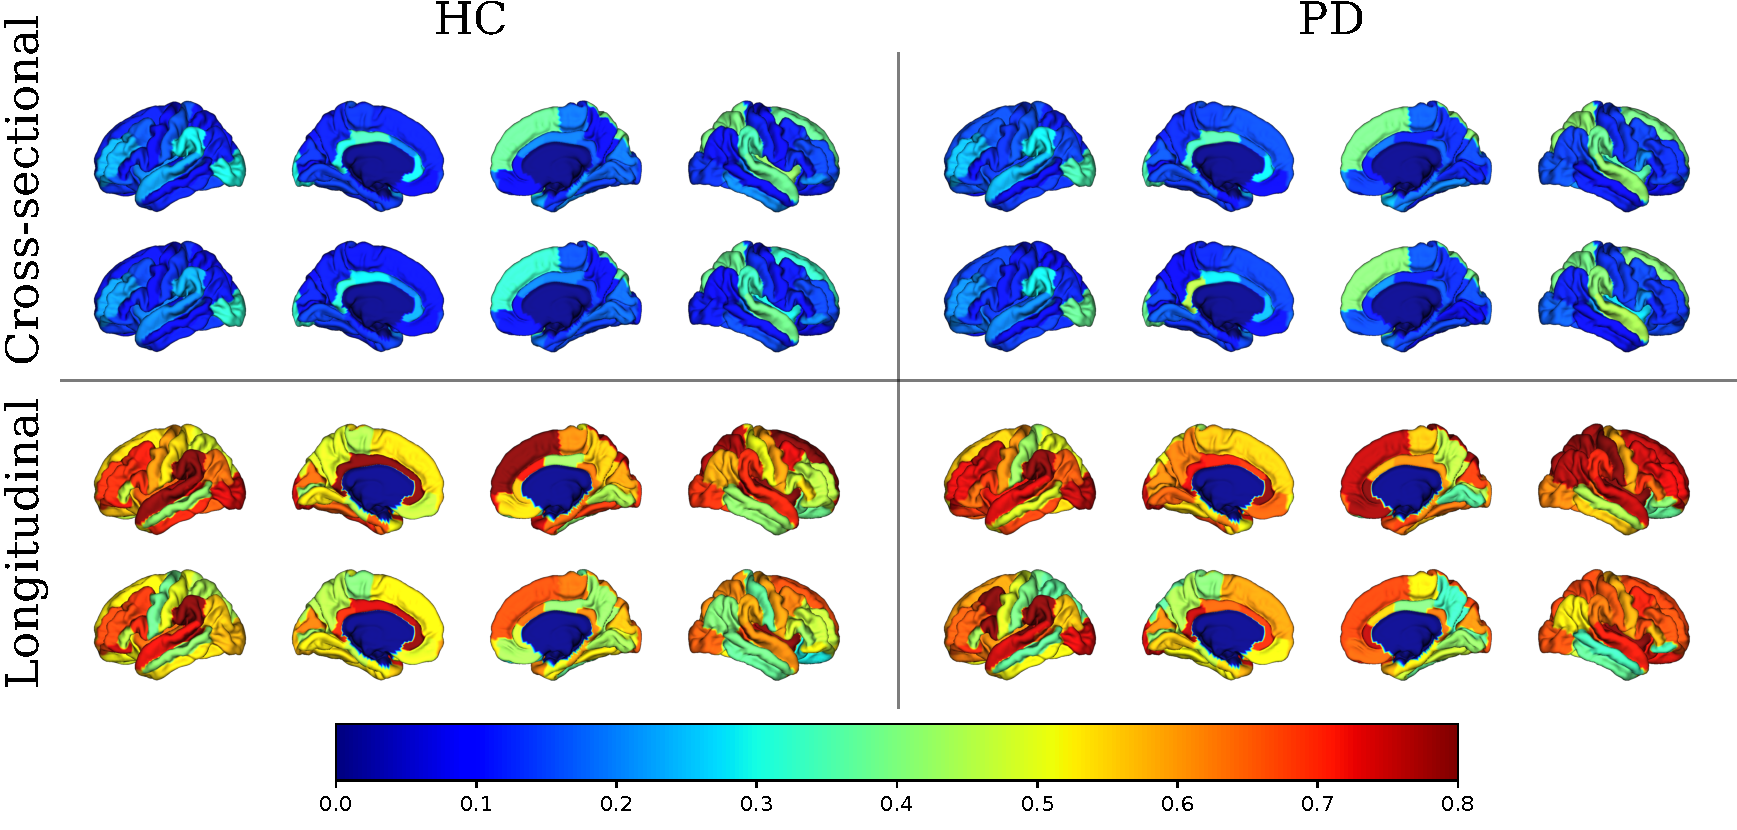
\includegraphics[width=\textwidth]{figures/NPV_map/figure_area_volume.pdf}
    \caption{Numerical-Population Variability Ratio (\navr) for cortical surface
        (top row in each panel) area and cortical volume (bottom row) in HC and
        PD. Panels show \navr{} maps at baseline for PD (a) and (HC),
        longitudinally for HC (c) and PD (d). Higher \navr{} values indicate
        greater computational uncertainty relative to inter-subject anatomical
        variability. Warmer colors denote higher \navr{} values.}
    \label{fig:navr_maps_area_volume}
\end{figure}

\subsection{Consistency results}

We evaluated the stability of statistical inferences by quantifying the
frequency of significance flipping across 26 MCA repetitions
(Table~\ref{tab:fluctuating_regions}). The analysis revealed that longitudinal
processing introduces considerably more instability than baseline
cross-sectional analysis, particularly for cortical metrics. Notably, partial
correlation analysis exhibited higher susceptibility to instability in cortical
volume (53\% of regions unstable) and area (38\% unstable) compared to ANCOVA.

To investigate whether longitudinal processing amplifies numerical instability,
we compared the dispersion of the test statistics ($F$-values for ANCOVA,
correlation coefficients $r$ for partial correlation) in longitudinal versus
cross-sectional pipelines. We used a one-sided Ansari-Bradley test on
mean-centered distributions to test the specific hypothesis that longitudinal
processing significantly has higher numerical variance compared to the baseline
(Tables~\ref{tab:stats-coef-var-subcortical} and
\ref{tab:stats-coef-var-cortical}).

For subcortical structures (Table~\ref{tab:stats-coef-var-subcortical}), partial
correlation yielded significantly higher variance in the longitudinal setting
for nearly all regions (13/14), whereas ANCOVA remained largely stable, with
only the caudate showing significant variance inflation. This trend was mirrored
in cortical regions (Table~\ref{tab:stats-coef-var-cortical}); partial
correlation analysis consistently demonstrated significantly greater variance
longitudinally across volume, thickness, and surface area. In contrast, ANCOVA
showed significant variance differences in far fewer regions.

\begin{table}[ht]
    \centering
    \small
    \setlength{\tabcolsep}{6pt}
    \renewcommand{\arraystretch}{1.15}
    \caption{Variance variability in subcortical structures
        (Ansari-Bradley test). Comparison of cross-sectional vs. longitudinal
        variances of test statistics. Significant results (*) indicate that
        longitudinal variance is significantly greater than baseline variance
        ($p_{\text{FDR}} < 0.05$, one-sided). $W$: test statistic.}
    \label{tab:fluctuating_regions}
    \begin{tabular}{lcccc}
        \hline
        \multirow{2}{*}{\textbf{Metric}}    &
        \multicolumn{2}{c}{\textbf{ANCOVA}} &
        \multicolumn{2}{c}{\textbf{Partial correlation}}                                                                            \\
        \cline{2-5}
                                            & \textbf{Baseline} & \textbf{Longitudinal} & \textbf{Baseline} & \textbf{Longitudinal} \\
        \hline
        Cortical Area (68 regions)          & 18 (27\%)         & 36 (53\%)             & 4 (6\%)           & 26 (38\%)             \\
        Cortical Thickness (68 regions)     & 11 (16\%)         & 9 (13\%)              & 19 (28\%)         & 17 (25\%)             \\
        Cortical Volume (68 regions)        & 14 (20\%)         & 20 (29\%)             & 8 (12\%)          & 36 (53\%)             \\
        Subcortical Volume (14 regions)     & 4 (29\%)          & 2 (14\%)              & 4 (29\%)          & 5 (36\%)              \\
        \hline
    \end{tabular}
\end{table}

% Table 1: Subcortical Structures
\begin{table}[h]
    \centering
    \centering
    \caption={Variance variability in cortical regions. One-sided
    Ansari-Bradley test comparing cross-sectional vs. longitudinal variances of
    test statistics. ($* p_{\text{FDR}} < 0.05$). L/R =
    Left/Right.  $W$ = statistic, $p$ = p-value.}
    \label{tab:stats-coef-var-subcortical}
    \begin{tblr}[
        ]
        {
            width = \textwidth,
            colspec = {l | Q[c,m] Q[c,m] | Q[c,m] Q[c,m]},
            row{odd} = {gray9},
            row{even} = {white},
            row{1} = {font=\bfseries, white},
            row{2} = {font=\bfseries, gray9},
            rows = {rowsep=0pt},
            rowhead = 2,
        }
        \hline
        \SetCell[r=2]{m} Region & \SetCell[c=2]{c} ANCOVA &          & \SetCell[c=2]{c} Partial Corr &         \\
        \hline
                                & W                       & p        & W                             & p       \\
        \hline
        L-Thalamus              & 248                     & 1.00     & 465                           & 6.1e-6* \\
        L-Caudate               & 501                     & 3.1e-10* & 459                           & 2.0e-5* \\
        L-Putamen               & 327                     & 0.81     & 491                           & 9.6e-9* \\
        L-Pallidum              & 264                     & 1.00     & 449                           & 1.1e-4* \\
        L-Hippocampus           & 314                     & 0.91     & 428                           & 2.2e-3* \\
        L-Amygdala              & 261                     & 1.00     & 476                           & 5.5e-7* \\
        L-Accumbens             & 265                     & 1.00     & 442                           & 3.3e-4* \\
        R-Thalamus              & 281                     & 1.00     & 441                           & 3.9e-4* \\
        R-Caudate               & 485                     & 5.5e-8*  & 478                           & 3.4e-7* \\
        R-Putamen               & 294                     & 0.98     & 489                           & 1.7e-8* \\
        R-Pallidum              & 212                     & 1.00     & 469                           & 2.7e-6* \\
        R-Hippocampus           & 335                     & 0.73     & 493                           & 5.1e-9* \\
        R-Amygdala              & 316                     & 0.90     & 408                           & 1.9e-2* \\
        R-Accumbens             & 214                     & 1.00     & 418                           & 7.0e-3* \\
        \hline
    \end{tblr}
\end{table}

% Table 2: Cortical Regions
\begin{longtblr}[
        caption={Ansari-Bradley test results for cross-sectional vs. longitudinal variances in cortical regions. * indicates FDR-corrected significance ($p < 0.05$). lh/rh =
                left/right hemisphere. ACC = anterior cingulate cortex, MF = middle
                frontal. $W$ = statistic, $p$ = p-value.},
        label={tab:stats-coef-var-cortical},
    ]{
        width=\linewidth,
        colspec = {l | *{4}{Q[c,m]} | *{4}{Q[c,m]} | *{4}{Q[c,m]}},
        row{odd} = {gray9},
        row{even} = {white},
        row{1} = {font=\bfseries, white},
        row{2} = {font=\bfseries, gray9},
        row{3} = {font=\bfseries, white},
        rows = {font=\footnotesize, rowsep=0pt},
        rowhead = 3,
    }
    \hline
    \SetCell[r=3]{m} Region   & \SetCell[c=4]{c} Cortical Volume &          &                               &          & \SetCell[c=4]{c} Cortical Thickness &          &                               &         & \SetCell[c=4]{c} Cortical Area &          &                               &          \\
    \hline
                              & \SetCell[c=2]{c} ANCOVA          &          & \SetCell[c=2]{c} Partial Corr &          & \SetCell[c=2]{c} ANCOVA             &          & \SetCell[c=2]{c} Partial Corr &         & \SetCell[c=2]{c} ANCOVA        &          & \SetCell[c=2]{c} Partial Corr &          \\
    \hline
                              & W                                & p        & W                             & p        & W                                   & p        & W                             & p       & W                              & p        & W                             & p        \\
    \hline
    bankssts (lh)             & 447                              & 1.6e-4*  & 486                           & 4.1e-8*  & 454                                 & 4.8e-5*  & 433                           & 1.2e-3* & 455                            & 4.1e-5*  & 481                           & 1.6e-7*  \\
    bankssts (rh)             & 403                              & 2.9e-2   & 466                           & 5.0e-6*  & 469                                 & 2.7e-6*  & 449                           & 1.1e-4* & 447                            & 1.6e-4*  & 461                           & 1.3e-5*  \\
    caudalACC (lh)            & 446                              & 1.8e-4*  & 487                           & 3.1e-8*  & 322                                 & 0.86     & 475                           & 6.9e-7* & 350                            & 0.52     & 480                           & 2.0e-7*  \\
    caudalACC (rh)            & 327                              & 0.81     & 513                           & 1.1e-12* & 501                                 & 3.1e-10* & 453                           & 5.8e-5* & 304                            & 0.96     & 500                           & 4.6e-10* \\
    caudalMF (lh)             & 437                              & 6.8e-4*  & 420                           & 5.6e-3*  & 479                                 & 2.6e-7*  & 413                           & 1.2e-2  & 362                            & 0.35     & 461                           & 1.3e-5*  \\
    caudalMF (rh)             & 439                              & 5.2e-4*  & 479                           & 2.6e-7*  & 352                                 & 0.49     & 445                           & 2.1e-4* & 390                            & 8.0e-2   & 489                           & 1.7e-8*  \\
    cuneus (lh)               & 441                              & 3.9e-4*  & 471                           & 1.7e-6*  & 507                                 & 2.6e-11* & 454                           & 4.8e-5* & 486                            & 4.1e-8*  & 483                           & 9.4e-8*  \\
    cuneus (rh)               & 387                              & 9.8e-2   & 481                           & 1.6e-7*  & 474                                 & 8.7e-7*  & 461                           & 1.3e-5* & 497                            & 1.4e-9*  & 487                           & 3.1e-8*  \\
    entorhinal (lh)           & 359                              & 0.39     & 409                           & 1.7e-2   & 297                                 & 0.98     & 396                           & 5.2e-2  & 474                            & 8.7e-7*  & 434                           & 1.0e-3*  \\
    entorhinal (rh)           & 372                              & 0.23     & 428                           & 2.2e-3*  & 246                                 & 1.00     & 396                           & 5.2e-2  & 505                            & 6.2e-11* & 455                           & 4.1e-5*  \\
    fusiform (lh)             & 477                              & 4.3e-7*  & 447                           & 1.6e-4*  & 421                                 & 5.0e-3*  & 419                           & 6.3e-3* & 421                            & 5.0e-3*  & 455                           & 4.1e-5*  \\
    fusiform (rh)             & 457                              & 2.8e-5*  & 460                           & 1.6e-5*  & 423                                 & 4.0e-3*  & 437                           & 6.8e-4* & 475                            & 6.9e-7*  & 454                           & 4.8e-5*  \\
    inferiorparietal (lh)     & 477                              & 4.3e-7*  & 503                           & 1.4e-10* & 347                                 & 0.56     & 458                           & 2.4e-5* & 487                            & 3.1e-8*  & 471                           & 1.7e-6*  \\
    inferiorparietal (rh)     & 369                              & 0.26     & 427                           & 2.5e-3*  & 460                                 & 1.6e-5*  & 383                           & 0.13    & 409                            & 1.7e-2   & 455                           & 4.1e-5*  \\
    inferiortemporal (lh)     & 437                              & 6.8e-4*  & 444                           & 2.5e-4*  & 356                                 & 0.44     & 461                           & 1.3e-5* & 472                            & 1.4e-6*  & 444                           & 2.5e-4*  \\
    inferiortemporal (rh)     & 335                              & 0.73     & 406                           & 2.3e-2   & 326                                 & 0.82     & 457                           & 2.8e-5* & 375                            & 0.20     & 456                           & 3.4e-5*  \\
    isthmuscingulate (lh)     & 432                              & 1.3e-3*  & 504                           & 9.5e-11* & 515                                 & 3.1e-13* & 462                           & 1.1e-5* & 413                            & 1.2e-2   & 505                           & 6.2e-11* \\
    isthmuscingulate (rh)     & 494                              & 3.7e-9*  & 469                           & 2.7e-6*  & 489                                 & 1.7e-8*  & 455                           & 4.1e-5* & 513                            & 1.1e-12* & 474                           & 8.7e-7*  \\
    lateraloccipital (lh)     & 494                              & 3.7e-9*  & 470                           & 2.1e-6*  & 430                                 & 1.7e-3*  & 440                           & 4.5e-4* & 475                            & 6.9e-7*  & 460                           & 1.6e-5*  \\
    lateraloccipital (rh)     & 472                              & 1.4e-6*  & 454                           & 4.8e-5*  & 498                                 & 9.5e-10* & 412                           & 1.3e-2  & 471                            & 1.7e-6*  & 461                           & 1.3e-5*  \\
    lateralorbitofrontal (lh) & 265                              & 1.00     & 414                           & 1.1e-2   & 184                                 & 1.00     & 464                           & 7.5e-6* & 294                            & 0.98     & 440                           & 4.5e-4*  \\
    lateralorbitofrontal (rh) & 271                              & 1.00     & 478                           & 3.4e-7*  & 422                                 & 4.5e-3*  & 429                           & 2.0e-3* & 258                            & 1.00     & 468                           & 3.3e-6*  \\
    lingual (lh)              & 250                              & 1.00     & 463                           & 9.1e-6*  & 494                                 & 3.7e-9*  & 468                           & 3.3e-6* & 453                            & 5.8e-5*  & 497                           & 1.4e-9*  \\
    lingual (rh)              & 435                              & 9.0e-4*  & 460                           & 1.6e-5*  & 480                                 & 2.0e-7*  & 467                           & 4.1e-6* & 477                            & 4.3e-7*  & 459                           & 2.0e-5*  \\
    medialorbitofrontal (lh)  & 459                              & 2.0e-5*  & 467                           & 4.1e-6*  & 479                                 & 2.6e-7*  & 410                           & 1.6e-2  & 396                            & 5.2e-2   & 469                           & 2.7e-6*  \\
    medialorbitofrontal (rh)  & 395                              & 5.6e-2   & 484                           & 7.2e-8*  & 300                                 & 0.97     & 430                           & 1.7e-3* & 405                            & 2.5e-2   & 459                           & 2.0e-5*  \\
    middletemporal (lh)       & 488                              & 2.3e-8*  & 487                           & 3.1e-8*  & 252                                 & 1.00     & 419                           & 6.3e-3* & 457                            & 2.8e-5*  & 464                           & 7.5e-6*  \\
    middletemporal (rh)       & 352                              & 0.49     & 463                           & 9.1e-6*  & 396                                 & 5.2e-2   & 428                           & 2.2e-3* & 427                            & 2.5e-3*  & 450                           & 9.5e-5*  \\
    parahippocampal (lh)      & 502                              & 2.1e-10* & 476                           & 5.5e-7*  & 462                                 & 1.1e-5*  & 437                           & 6.8e-4* & 425                            & 3.2e-3*  & 463                           & 9.1e-6*  \\
    parahippocampal (rh)      & 473                              & 1.1e-6*  & 468                           & 3.3e-6*  & 349                                 & 0.54     & 458                           & 2.4e-5* & 415                            & 9.6e-3*  & 459                           & 2.0e-5*  \\
    paracentral (lh)          & 314                              & 0.91     & 424                           & 3.6e-3*  & 204                                 & 1.00     & 425                           & 3.2e-3* & 491                            & 9.6e-9*  & 438                           & 6.0e-4*  \\
    paracentral (rh)          & 331                              & 0.77     & 484                           & 7.2e-8*  & 280                                 & 1.00     & 441                           & 3.9e-4* & 330                            & 0.78     & 485                           & 5.5e-8*  \\
    parsopercularis (lh)      & 362                              & 0.35     & 461                           & 1.3e-5*  & 494                                 & 3.7e-9*  & 418                           & 7.0e-3* & 459                            & 2.0e-5*  & 472                           & 1.4e-6*  \\
    parsopercularis (rh)      & 388                              & 9.1e-2   & 482                           & 1.2e-7*  & 305                                 & 0.96     & 477                           & 4.3e-7* & 447                            & 1.6e-4*  & 466                           & 5.0e-6*  \\
    parsorbitalis (lh)        & 293                              & 0.98     & 490                           & 1.3e-8*  & 230                                 & 1.00     & 462                           & 1.1e-5* & 419                            & 6.3e-3*  & 462                           & 1.1e-5*  \\
    parsorbitalis (rh)        & 295                              & 0.98     & 455                           & 4.1e-5*  & 336                                 & 0.71     & 427                           & 2.5e-3* & 269                            & 1.00     & 471                           & 1.7e-6*  \\
    parstriangularis (lh)     & 339                              & 0.68     & 507                           & 2.6e-11* & 401                                 & 3.5e-2   & 419                           & 6.3e-3* & 419                            & 6.3e-3*  & 504                           & 9.5e-11* \\
    parstriangularis (rh)     & 404                              & 2.7e-2   & 455                           & 4.1e-5*  & 288                                 & 0.99     & 394                           & 6.0e-2  & 362                            & 0.35     & 463                           & 9.1e-6*  \\
    pericalcarine (lh)        & 442                              & 3.3e-4*  & 465                           & 6.1e-6*  & 441                                 & 3.9e-4*  & 470                           & 2.1e-6* & 460                            & 1.6e-5*  & 509                           & 9.9e-12* \\
    pericalcarine (rh)        & 390                              & 8.0e-2   & 449                           & 1.1e-4*  & 480                                 & 2.0e-7*  & 451                           & 8.1e-5* & 443                            & 2.9e-4*  & 492                           & 7.0e-9*  \\
    postcentral (lh)          & 329                              & 0.79     & 460                           & 1.6e-5*  & 331                                 & 0.77     & 423                           & 4.0e-3* & 372                            & 0.23     & 477                           & 4.3e-7*  \\
    postcentral (rh)          & 350                              & 0.52     & 449                           & 1.1e-4*  & 269                                 & 1.00     & 426                           & 2.8e-3* & 514                            & 6.1e-13* & 387                           & 9.8e-2   \\
    posteriorcingulate (lh)   & 317                              & 0.90     & 488                           & 2.3e-8*  & 487                                 & 3.1e-8*  & 436                           & 7.9e-4* & 328                            & 0.80     & 465                           & 6.1e-6*  \\
    posteriorcingulate (rh)   & 315                              & 0.91     & 478                           & 3.4e-7*  & 480                                 & 2.0e-7*  & 450                           & 9.5e-5* & 356                            & 0.44     & 485                           & 5.5e-8*  \\
    precentral (lh)           & 284                              & 0.99     & 457                           & 2.8e-5*  & 239                                 & 1.00     & 372                           & 0.23    & 444                            & 2.5e-4*  & 424                           & 3.6e-3*  \\
    precentral (rh)           & 325                              & 0.83     & 420                           & 5.6e-3*  & 312                                 & 0.93     & 387                           & 9.8e-2  & 470                            & 2.1e-6*  & 488                           & 2.3e-8*  \\
    precuneus (lh)            & 240                              & 1.00     & 408                           & 1.9e-2   & 251                                 & 1.00     & 483                           & 9.4e-8* & 410                            & 1.6e-2   & 430                           & 1.7e-3*  \\
    precuneus (rh)            & 288                              & 0.99     & 414                           & 1.1e-2   & 244                                 & 1.00     & 465                           & 6.1e-6* & 363                            & 0.34     & 457                           & 2.8e-5*  \\
    rostralACC (lh)           & 269                              & 1.00     & 436                           & 7.9e-4*  & 505                                 & 6.2e-11* & 467                           & 4.1e-6* & 353                            & 0.48     & 460                           & 1.6e-5*  \\
    rostralACC (rh)           & 275                              & 1.00     & 501                           & 3.1e-10* & 481                                 & 1.6e-7*  & 448                           & 1.3e-4* & 275                            & 1.00     & 448                           & 1.3e-4*  \\
    rostralmiddlefrontal (lh) & 370                              & 0.25     & 482                           & 1.2e-7*  & 276                                 & 1.00     & 430                           & 1.7e-3* & 283                            & 0.99     & 489                           & 1.7e-8*  \\
    rostralmiddlefrontal (rh) & 318                              & 0.89     & 418                           & 7.0e-3*  & 319                                 & 0.88     & 431                           & 1.5e-3* & 219                            & 1.00     & 442                           & 3.3e-4*  \\
    superiorfrontal (lh)      & 370                              & 0.25     & 443                           & 2.9e-4*  & 456                                 & 3.4e-5*  & 464                           & 7.5e-6* & 481                            & 1.6e-7*  & 435                           & 9.0e-4*  \\
    superiorfrontal (rh)      & 392                              & 6.9e-2   & 432                           & 1.3e-3*  & 271                                 & 1.00     & 467                           & 4.1e-6* & 376                            & 0.19     & 480                           & 2.0e-7*  \\
    superiorparietal (lh)     & 369                              & 0.26     & 333                           & 0.75     & 369                                 & 0.26     & 440                           & 4.5e-4* & 489                            & 1.7e-8*  & 386                           & 0.10     \\
    superiorparietal (rh)     & 506                              & 4.0e-11* & 430                           & 1.7e-3*  & 437                                 & 6.8e-4*  & 463                           & 9.1e-6* & 456                            & 3.4e-5*  & 430                           & 1.7e-3*  \\
    superiortemporal (lh)     & 413                              & 1.2e-2   & 484                           & 7.2e-8*  & 427                                 & 2.5e-3*  & 441                           & 3.9e-4* & 446                            & 1.8e-4*  & 481                           & 1.6e-7*  \\
    superiortemporal (rh)     & 401                              & 3.5e-2   & 452                           & 6.8e-5*  & 364                                 & 0.32     & 469                           & 2.7e-6* & 425                            & 3.2e-3*  & 470                           & 2.1e-6*  \\
    supramarginal (lh)        & 466                              & 5.0e-6*  & 466                           & 5.0e-6*  & 274                                 & 1.00     & 488                           & 2.3e-8* & 509                            & 9.9e-12* & 481                           & 1.6e-7*  \\
    supramarginal (rh)        & 394                              & 6.0e-2   & 422                           & 4.5e-3*  & 483                                 & 9.4e-8*  & 412                           & 1.3e-2  & 376                            & 0.19     & 432                           & 1.3e-3*  \\
    frontalpole (lh)          & 385                              & 0.11     & 445                           & 2.1e-4*  & 319                                 & 0.88     & 453                           & 5.8e-5* & 347                            & 0.56     & 428                           & 2.2e-3*  \\
    frontalpole (rh)          & 284                              & 0.99     & 410                           & 1.6e-2   & 391                                 & 7.5e-2   & 451                           & 8.1e-5* & 218                            & 1.00     & 399                           & 4.1e-2   \\
    temporalpole (lh)         & 356                              & 0.44     & 379                           & 0.16     & 308                                 & 0.94     & 384                           & 0.12    & 385                            & 0.11     & 436                           & 7.9e-4*  \\
    temporalpole (rh)         & 252                              & 1.00     & 344                           & 0.61     & 421                                 & 5.0e-3*  & 403                           & 2.9e-2  & 225                            & 1.00     & 396                           & 5.2e-2   \\
    transversetemporal (lh)   & 406                              & 2.3e-2   & 467                           & 4.1e-6*  & 367                                 & 0.29     & 421                           & 5.0e-3* & 445                            & 2.1e-4*  & 482                           & 1.2e-7*  \\
    transversetemporal (rh)   & 324                              & 0.84     & 417                           & 7.8e-3*  & 477                                 & 4.3e-7*  & 442                           & 3.3e-4* & 347                            & 0.56     & 435                           & 9.0e-4*  \\
    insula (lh)               & 249                              & 1.00     & 470                           & 2.1e-6*  & 220                                 & 1.00     & 457                           & 2.8e-5* & 263                            & 1.00     & 438                           & 6.0e-4*  \\
    insula (rh)               & 267                              & 1.00     & 444                           & 2.5e-4*  & 401                                 & 3.5e-2   & 439                           & 5.2e-4* & 235                            & 1.00     & 410                           & 1.6e-2   \\
    \hline
\end{longtblr}

\begin{table}[t]
    \centering
    \caption{Permutation test comparison of $\nu_{\text{nav}}$ between HC and PD.
        No significance detected after Bonferroni correction ($\alpha=0.05/8$).
        Values are observed differences (PD$-$HC). 95\% CIs from percentile bootstrap.}
    \label{tab:bootstrap-navr}
    \begin{tabular}{lcccc}
        \toprule
        \textbf{Metric}    & {\textbf{Observed} $\Delta$} & \textbf{95\% CI}    & {\textbf{p-value}} & \textbf{Study}  \\
        \midrule
        area               & 0.005                        & {[}-0.002, 0.013{]} & 0.734              & cross-sectional \\
        thickness          & 0.027                        & {[}0.020, 0.034{]}  & 0.033              & cross-sectional \\
        volume             & 0.013                        & {[} 0.004, 0.022{]} & 0.371              & cross-sectional \\
        subcortical volume & 0.014                        & {[} 0.004, 0.025{]} & 0.646              & cross-sectional \\
        \midrule
        area               & 0.021                        & {[}-0.002, 0.044{]} & 0.482              & longitudinal    \\
        thickness          & 0.002                        & {[}-0.014, 0.020{]} & 0.919              & longitudinal    \\
        volume             & 0.025                        & {[} 0.002, 0.049{]} & 0.370              & longitudinal    \\
        subcortical volume & -0.027                       & {[}-0.047,-0.006{]} & 0.489              & longitudinal    \\
        \bottomrule
    \end{tabular}
\end{table}

\subsubsection{Consistency of statistical tests}

For both group comparisons and correlation analyses, statistical outcomes varied
substantially across the 26 Monte Carlo Arithmetic (MCA) repetitions (Figures
\ref{fig:navr_consistency_area_plot} and \ref{fig:consistency_volume_plot}). For
cortical area (68 regions; Figure \ref{fig:navr_consistency_area_plot}),
significance flipped in 31\% of all (regions, analysis) pairs, indicating
frequent inconsistencies across repetitions. For cortical volume (68 regions;
Figure \ref{fig:consistency_volume_plot}), 29\% of pairs were similarly unstable.
These fluctuations demonstrate that numerical noise alone can alter downstream
statistical inference in structural MRI analyses of PD.

\begin{figure}[h]
    \centering
    \includegraphics[width=\linewidth]{figures/consistency/cortical_area_significance_correlation.pdf}
    \caption{Consistency of statistical tests for cortical area across all
        subjects and regions. The plot shows the percentage of subjects for
        which the statistical test was significant ($\alpha = 0.05$) for each
        region. The consistency varies across regions, with some regions showing
        higher consistency than others.}
    \label{fig:navr_consistency_area_plot}
\end{figure}

\begin{figure}[h]
    \centering
    \includegraphics[width=\linewidth]{figures/consistency/cortical_volume_significance_correlation.pdf}
    \caption{Consistency of statistical tests for cortical volume across all
        subjects and regions. The plot shows the percentage of subjects for
        which the statistical test was significant ($\alpha = 0.05$) for each
        region. The consistency varies across regions, with some regions showing
        higher consistency than others.}
    \label{fig:consistency_volume_plot}
\end{figure}

\subsection{Interactive web tool}

\begin{figure}[ht]
    \centering
    \includegraphics[width=0.7\linewidth]{figures/screenshot_light.png}
    \caption{Interactive web tool for estimating NPVR and assessing numerical
        variability in neuroimaging studies. Users can input summary statistics
        to obtain NPVR values and visualize the impact of numerical variability
        on effect size estimates. The tool is available at
        \href{https://yohanchatelain.github.io/brain\_render/}{yohanchatelain.github.io/brain\_render}.
        \label{fig:brain_render_tool}}
\end{figure}

\section{Distribution of statistical tests coefficients}
\label{appendix:distribution_stats_ieee}

Figures \ref{fig:statstest_coefficients_distribution},
\ref{fig:consistency_area_coefficients} and
\ref{fig:consistency_volume_coefficients} show the distribution of partial
correlation coefficients and F-statistics for subcortical volume measures,
cortical thickness, cortical areas and cortical volumes, across all subjects
and regions. Red triangles indicate the unperturbed (IEEE-754) run for
reference. For all analyses, the unperturbed (IEEE-754) result is included in
the range of numericallly perturbed results, which supports the validity of the
numerical perturbation.

% The distribution shows the variability in the
% coefficients, with some regions exhibiting higher consistency than others.

% For subcortical volumes, the distributions of partial-correlation coefficients
% ($r$) and ANCOVA $F$-statistics
% (Figure~\ref{fig:statstest_coefficients_distribution}) show that the unperturbed
% IEEE-754 estimates (red markers) consistently fall within the MCA-sampled range.
% This supports the validity of the instrumentation rather than indicating a
% methodological artifact. The spread of the $r$ coefficients is larger in
% longitudinal than in baseline analyses (Ansari-Bradley one-sided test at
% $p<0.05$ corrected with Bonferroni; detailed results in Appendix
% Table~\ref{tab:stats-coef-var-subcortical}), whereas no significant difference
% in spread is detected for $F$-statistics using the same test
% (Bonferroni-corrected, $p<0.05$). This indicates that numerical variability has
% a more pronounced impact on longitudinal studies than on cross-sectional ones.
% An analogous analysis for cortical thickness leads to similar conclusions
% (Appendix Figure~\ref{fig:consistency_thickness_coefficients},
% Table~\ref{tab:stats-coef-var-cortical}).

\begin{figure}[ht]
    \centering
    \includegraphics[width=\linewidth]{figures/consistency/subcortical_volume_coefficients_distribution.pdf}
    \caption{ Distribution of partial correlation coefficients (r-values) and
        F-statistics from ANCOVA across MCA repetitions for subcortical volume
        measures. Red dots represent the IEEE-754 unperturbed results.
        \label{fig:statstest_coefficients_distribution}}
\end{figure}

\begin{figure}
    \centering
    \begin{subfigure}[b]{\linewidth}
        \centering
        \includegraphics[width=.9\linewidth]{figures/consistency/cortical_thickness_coefficients_distribution-Left.pdf}
        \caption{Left hemisphere}
        \label{fig:consistency_thickness_left}
    \end{subfigure}

    \begin{subfigure}[b]{\linewidth}
        \centering
        \includegraphics[width=.9\linewidth]{figures/consistency/cortical_thickness_coefficients_distribution-Right.pdf}
        \caption{Right hemisphere}
        \label{fig:consistency_thickness_right}
    \end{subfigure}
    \caption{Distribution of partial correlation coefficients for cortical
        thickness across all subjects and regions. Red triangles indicate the
        IEEE-754 run for reference. }
    \label{fig:consistency_thickness_coefficients}
\end{figure}

\begin{figure}[h]
    \centering
    \begin{subfigure}[b]{\linewidth}
        \centering
        \includegraphics[width=.9\linewidth]{figures/consistency/cortical_area_coefficients_distribution-Left.pdf}
        \caption{Left hemisphere}
        \label{fig:consistency_area_left}
    \end{subfigure}
    \hfill
    \begin{subfigure}[b]{\linewidth}
        \centering
        \includegraphics[width=.9\linewidth]{figures/consistency/cortical_area_coefficients_distribution-Right.pdf}
        \caption{Right hemisphere}
        \label{fig:consistency_area_right}
    \end{subfigure}
    \caption{ Distribution of partial correlation coefficients for cortical surface area
        across all subjects and regions. Red triangles indicate the IEEE-754 run
        for reference. }
    \label{fig:consistency_area_coefficients}
\end{figure}

\begin{figure}[h]
    \centering
    \begin{subfigure}[b]{\linewidth}
        \centering
        \includegraphics[width=.9\linewidth]{figures/consistency/cortical_volume_coefficients_distribution-Left.pdf}
        \caption{Left hemisphere}
        \label{fig:consistency_volume_left}
    \end{subfigure}
    \hfill
    \begin{subfigure}[b]{\linewidth}
        \centering
        \includegraphics[width=.9\linewidth]{figures/consistency/cortical_volume_coefficients_distribution-Right.pdf}
        \caption{Right hemisphere}
        \label{fig:consistency_volume_right}
    \end{subfigure}
    \caption{ Distribution of partial correlation coefficients for cortical
        volume across all subjects and regions. Red triangles indicate the
        IEEE-754 run for reference. The distribution shows the variability in
        the coefficients, with some regions exhibiting higher consistency than
        others.}
    \label{fig:consistency_volume_coefficients}
\end{figure}

\begin{figure}[h]
    \centering
    \vspace{0.2cm}

    % Header row with column labels
    \begin{minipage}[b]{\linewidth}
        \begin{minipage}[c]{0.05\linewidth}
            % Empty space for alignment with condition labels
        \end{minipage}%
        \begin{minipage}[c]{0.95\linewidth}
            \begin{minipage}[c]{0.47\linewidth}
                \centering\textbf{Unthresholded}
            \end{minipage}%
            \hfill
            \begin{minipage}[c]{0.005\linewidth}
                % Vertical line separator
            \end{minipage}%
            \hfill
            \begin{minipage}[c]{0.47\linewidth}
                \centering\textbf{Thresholded}
            \end{minipage}
        \end{minipage}
    \end{minipage}

    % Horizontal line
    \noindent\rule{\linewidth}{0.5pt}
    \vspace{-1.5cm}

    % 22q11.2 deletion syndrome row
    \begin{minipage}[b]{\linewidth}
        \begin{minipage}[c]{0.05\linewidth}
            \centering\rotatebox{90}{\textbf{22q11.2}} \end{minipage}%
        \begin{minipage}[c]{0.95\linewidth}
            \begin{subfigure}[c]{0.47\linewidth}
                \includegraphics[width=\linewidth]{figures/cohen_d_map/enigma/22q_area_all.png}
                \label{fig:enigma_22q_unthresholded}
            \end{subfigure}%
            \hfill
            \begin{minipage}[c]{0.005\linewidth}
                \centering\rule{0.5pt}{4cm}
            \end{minipage}%
            \hfill
            \begin{subfigure}[c]{0.47\linewidth}
                \includegraphics[width=\linewidth]{figures/cohen_d_map/enigma/22q_area_all_thresholded.png}
                \label{fig:enigma_22q_thresholded}
            \end{subfigure}
        \end{minipage}
    \end{minipage}

    \vspace{-2cm}

    % ADHD row
    \begin{minipage}[b]{\linewidth}
        \begin{minipage}[c]{0.05\linewidth}
            \centering\rotatebox{90}{\textbf{ADHD}} \end{minipage}%
        \begin{minipage}[c]{0.95\linewidth}
            \begin{subfigure}[c]{0.47\linewidth}
                \includegraphics[width=\linewidth]{figures/cohen_d_map/enigma/adhd_area_adult.png}
                \label{fig:enigma_adhd_unthresholded}
            \end{subfigure}%
            \hfill
            \begin{minipage}[c]{0.005\linewidth}
                \centering\rule{0.5pt}{4cm}
            \end{minipage}%
            \hfill
            \begin{subfigure}[c]{0.47\linewidth}
                \includegraphics[width=\linewidth]{figures/cohen_d_map/enigma/adhd_area_adult_thresholded.png}
                \label{fig:enigma_adhd_thresholded}
            \end{subfigure}
        \end{minipage}
    \end{minipage}

    \vspace{-2cm}

    % bipolar disorder row
    \begin{minipage}[b]{\linewidth}
        \begin{minipage}[c]{0.05\linewidth}
            \centering\rotatebox{90}{\textbf{Bipolar}} \end{minipage}%
        \begin{minipage}[c]{0.95\linewidth}
            \begin{subfigure}[c]{0.47\linewidth}
                \includegraphics[width=\linewidth]{figures/cohen_d_map/enigma/bipolar_area_adult.png}
                \label{fig:enigma_bipolar_unthresholded}
            \end{subfigure}%
            \hfill
            \begin{minipage}[c]{0.005\linewidth}
                \centering\rule{0.5pt}{4cm}
            \end{minipage}%
            \hfill
            \begin{subfigure}[c]{0.47\linewidth}
                \includegraphics[width=\linewidth]{figures/cohen_d_map/enigma/bipolar_area_adult_thresholded.png}
                \label{fig:enigma_bipolar_thresholded}
            \end{subfigure}
        \end{minipage}
    \end{minipage}

    \vspace{-2cm}
    % depression
    \begin{minipage}[b]{\linewidth}
        \begin{minipage}[c]{0.05\linewidth}
            \centering\rotatebox{90}{\textbf{Depression}} \end{minipage}%
        \begin{minipage}[c]{0.95\linewidth}
            \begin{subfigure}[c]{0.47\linewidth}
                \includegraphics[width=\linewidth]{figures/cohen_d_map/enigma/depression_area_adult.png}
                \label{fig:enigma_depression_unthresholded}
            \end{subfigure}%
            \hfill
            \begin{minipage}[c]{0.005\linewidth}
                \centering\rule{0.5pt}{4cm}
            \end{minipage}%
            \hfill
            \begin{subfigure}[c]{0.47\linewidth}
                \includegraphics[width=\linewidth]{figures/cohen_d_map/enigma/depression_area_adult_thresholded.png}
                \label{fig:enigma_depression_thresholded}
            \end{subfigure}
        \end{minipage}
    \end{minipage}

    \vspace{-2cm}
    % ocd 
    \begin{minipage}[b]{\linewidth}
        \begin{minipage}[c]{0.05\linewidth}
            \centering\rotatebox{90}{\textbf{OCD}} \end{minipage}%
        \begin{minipage}[c]{0.95\linewidth}
            \begin{subfigure}[c]{0.47\linewidth}
                \includegraphics[width=\linewidth]{figures/cohen_d_map/enigma/ocd_area_adult.png}
                \label{fig:enigma_ocd_unthresholded}
            \end{subfigure}%
            \hfill
            \begin{minipage}[c]{0.005\linewidth}
                \centering\rule{0.5pt}{4cm}
            \end{minipage}%
            \hfill
            \begin{subfigure}[c]{0.47\linewidth}
                \includegraphics[width=\linewidth]{figures/cohen_d_map/enigma/ocd_area_adult_thresholded.png}
                \label{fig:enigma_ocd_thresholded}
            \end{subfigure}
        \end{minipage}
    \end{minipage}

    \vspace{-2cm}
    % schizophrenia
    \begin{minipage}[b]{\linewidth}
        \begin{minipage}[c]{0.05\linewidth}
            \centering\rotatebox{90}{\textbf{Schizophrenia}} \end{minipage}%
        \begin{minipage}[c]{0.95\linewidth}
            \begin{subfigure}[c]{0.47\linewidth}
                \includegraphics[width=\linewidth]{figures/cohen_d_map/enigma/schizophrenia_area_all.png}
                \label{fig:enigma_schizophrenia_unthresholded}
            \end{subfigure}%
            \hfill
            \begin{minipage}[c]{0.005\linewidth}
                \centering\rule{0.5pt}{4cm}
            \end{minipage}%
            \hfill
            \begin{subfigure}[c]{0.47\linewidth}
                \includegraphics[width=\linewidth]{figures/cohen_d_map/enigma/schizophrenia_area_all_thresholded.png}
                \label{fig:enigma_schizophrenia_thresholded}
            \end{subfigure}
        \end{minipage}
    \end{minipage}

    \caption{ENIGMA cortical area Cohen's d maps showing unthresholded effect
        sizes (left) and effect sizes thresholded by the \navr framework (right)
        for different disorders. Black regions indicate areas where Cohen's d
        values fall below the numerical variability threshold, demonstrating
        regions where reported effect sizes may be unreliable due to
        computational uncertainty.}
    \label{fig:navr_enigma_area}
\end{figure}

\section{Numerical validation of flip significance simulations}
\label{appendix:numerical_validation_flip_significance}

To assess the validity of the analytical uncertainty framework used to model
numerically induced significance instability, we compared simulated estimates
derived from closed-form uncertainty expressions with empirical estimates
obtained from Monte Carlo Arithmetic (MCA) repetitions. Formally, the
proportion of significant tests (positive prediction rate, PPR) is defined as:
\begin{equation}
    \text{PPR} = \frac{\text{TP} + \text{FN}}{\text{TP} + \text{FP} + \text{TN} + \text{FN}},
    \label{eq:ppr}
\end{equation}
where TP, FP, TN, and FN denote true positives, false positives, true negatives,
and false negatives, respectively.

Figure~\ref{fig:std_sampled_simulated_comparison} compares standard deviations of
$p$-values estimated directly from 26 MCA runs with those predicted by the
analytical uncertainty formulas (Table~\ref{tab:stat_uncertainty}). Each point
corresponds to a cortical or subcortical brain region. Results show close
agreement between sampled and simulated estimates, particularly in the
cross-sectional setting. In the longitudinal analyses, simulated standard
deviations tend to be slightly larger than sampled values, indicating a
conservative bias of the analytical model.

Figure~\ref{fig:ppr_simulated_comparison} evaluates how this analytical
uncertainty propagates to downstream inference by comparing the simulated
positive prediction rate (PPR; Eq.~\ref{eq:ppr}) with the empirical proportion
of significant tests observed across MCA repetitions. Cross-sectional results
closely follow the identity line, while longitudinal results show a moderate
overestimation of PPR, consistent with the conservative overestimation of
$p$-value variability observed in Fig.~\ref{fig:std_sampled_simulated_comparison}.

Finally, Figure~\ref{fig:ppr_sampled_comparison} assesses the Beta distribution
model used to translate sampled $p$-value variability into PPR estimates.
Here, PPR is computed using MCA-derived standard deviations propagated through
the Beta model (Eq.~\ref{eq:beta-params}). Both cross-sectional and longitudinal
results align closely with the identity line, supporting the suitability of the
Beta modeling framework for capturing numerically induced variability in
statistical significance.

\begin{figure}[ht]
    \centering
    \includegraphics[width=.9\linewidth]{figures/std-sampled-simulated-comparison.pdf}
    \caption{Comparison of standard deviation estimates of $p$-values obtained from
        MCA sampling and analytical simulations. Sampled estimates are computed from
        26 MCA repetitions, while simulated estimates are derived from the
        uncertainty propagation formulas reported in
        Table~\ref{tab:stat_uncertainty}. Each point corresponds to a cortical or
        subcortical brain region. The solid line denotes the identity line. Results
        show close agreement between sampled and simulated estimates, with
        cross-sectional analyses exhibiting tighter clustering than longitudinal
        analyses. In the longitudinal setting, simulated standard deviations tend to
        slightly overestimate sampled variability, indicating conservative behavior
        of the analytical uncertainty model.
        \label{fig:std_sampled_simulated_comparison}}
\end{figure}

\begin{figure}[ht]
    \centering
    \includegraphics[width=.9\linewidth]{figures/ppr_simulated.pdf}
    \caption{ Comparison between simulated positive prediction rate (PPR;
        Eq.~\ref{eq:ppr}) and the empirical proportion of significant tests
        (Section~\ref{sec:empirical_evaluation}). Simulated PPR values are computed
        using analytical uncertainty estimates derived from
        Table~\ref{tab:stat_uncertainty}. Each point represents a cortical or
        subcortical brain region, and the solid line indicates the identity line.
        Simulated PPR closely matches empirical significance rates in the
        cross-sectional setting, while longitudinal analyses show a tendency toward
        overestimation, consistent with the corresponding overestimation of
        $p$-value variability.\label{fig:ppr_simulated_comparison}}
\end{figure}

\begin{figure}[ht]
    \centering
    \includegraphics[width=.9\linewidth]{figures/ppr_sampled.pdf}
    \caption{Comparison between sampled positive prediction rate (PPR;
        Eq.~\ref{eq:ppr}) and the empirical proportion of significant tests
        (Section~\ref{sec:empirical_evaluation}). Sampled PPR values are
        computed from MCA-derived $p$-value standard deviations and propagated
        through the Beta distribution model (Eq.~\ref{eq:beta-params}). Each
        point corresponds to a cortical or subcortical brain region, and the
        solid line denotes the identity line. Both cross-sectional and
        longitudinal results align closely with the identity line, supporting
        the suitability of the Beta modeling framework for capturing numerically
        induced variability in statistical significance.
        \label{fig:ppr_sampled_comparison}}
\end{figure}
}{}

\end{document}
